\documentclass[%
%%% PARA ESCOLHER O ESTILO TIRE O SIMBOLO %(COMENTÁRIO)
%SemVinculoColorido,
%SemFormatacaoCapitulo,
%SemFolhaAprovacao,
%SemImagens,
%CitacaoNumerica, %% o padrão é citação tipo autor-data
%PublicacaoDissOuTese, %% (é também o "default") com ficha catal. e folha de aprovação em branco. Caso tenha lista de símbolos e lista de siglas e abreviaturas retirar os comentários dos arquivos siglas.tex e abreviaturasesiglas.tex. Retirar também os comentários indicados nesse arquivo, nos includes
%PublicacaoArtigoOuRelatorio, %% texto sequencial, sem quebra de páginas nem folhas em branco
PublicacaoProposta, %% igual tese/dissertação, mas sem ficha catal. e fol. de aprov.
%PublicacaoLivro, %% com capítulos
%PublicacaoLivro,SemFormatacaoCapitulo, %% sem capítulos
english,portuguese %% para os documentos em Português com abstract.tex em Inglês
%portuguese,english %% para os documentos em Inglês com abstract.tex em Português
,LogoINPE% comentar essa linha para fazer aparecer o logo do Governo
,CCBYNC	% as opções de licença são: CCBY, CCBYSA, CCBYND, CCBYNC, CCBYNCSA, CCBYNCND, GPLv3 e INPECopyright
]{tdiinpe}
%]{../../../../../iconet.com.br/banon/2008/03.25.01.19/doc/tdiinpe}

% PARA EXIBIR EM ARIAL TIRAR O COMENTÁRIO DAS DUAS LINHAS SEGUINTES
%\renewcommand{\rmdefault}{phv} % Arial
%\renewcommand{\sfdefault}{phv} % Arial

% PARA PUBLICAÇÕES EM INGLÊS:
% renomear o arquivo: abnt-alf.bst para abnt-alfportuguese.bst
% renomear o arquivo: abnt-alfenglish.bst para abnt-alf.bst

%%%%%%%%%%%%%%%%%%%%%%%%%%%%%%%%%%%%%%%%%%%%%
%%% Pacotes já previamente carregados:      %
%%%%%%%%%%%%%%%%%%%%%%%%%%%%%%%%%%%%%%%%%%%%%%%%%%%%%%%%%%%%%%%%%%%%%%%%
%%% ifthen,calc,graphicx,color,inputenc,babel,hyphenat,array,setspace, %
%%% bigdelim,multirow,supertabular,tabularx,longtable,lastpage,lscape, %
%%% rotate,caption2,amsmath,amssymb,amsthm,subfigure,tocloft,makeidx,  %
%%% eso-pic,calligra,hyperref,ae,fontenc                               %
%%%%%%%%%%%%%%%%%%%%%%%%%%%%%%%%%%%%%%%%%%%%%%%%%%%%%%%%%%%%%%%%%%%%%%%%
%%% insira neste campo, comandos de LaTeX %%%
%%% \usepackage{_exemplo_}
% etc.
%%%%%%%%%%%%%%%%%%%%%%%%%%%%%%%%%%%%%%%%%%%%%

%\watermark{Revisão No. ##} %% use o comando \watermark para identificar a versão de seu documento
%% comente este comando quando for gerar a versão final

% Engana o pacote tcolorbox no carregamento do inputenc
% (https://tex.stackexchange.com/questions/370262/how-to-adapt-tcolorbox-with-xelatex)
\makeatletter\@namedef{ver@inputenc.sty}{}\makeatother

% Pacotes Extras
% Pacotes Extras
\usepackage{rotating}
\usepackage{dsfont}
\usepackage{comment}
\usepackage{xcolor}
\usepackage{xcolor-material}
\usepackage{xcolor-solarized}
\usepackage{minted}
\usemintedstyle{material}
\usepackage{multicol}
\usepackage{listings}
\usepackage{ulem}
\usepackage{cancel}
\usepackage{lipsum} % http://ctan.org/pkg/lipsum
\usepackage{graphicx}
\usepackage{pstricks}
\usepackage{pst-plot}
\usepackage{pst-3dplot}
%\usepackage{pst-exa}
\usepackage{booktabs}
\usepackage{wrapfig}

%\usetikzlibrary{decorations.pathmorphing}
%\usetikzlibrary{shadows}

%\usepackage{caption}
%\usepackage{subcaption}
%\usepackage{subfig}

%\definecolor{codegreen}{rgb}{0,0.6,0}
%\definecolor{codegray}{rgb}{0.5,0.5,0.5}
%\definecolor{codepurple}{rgb}{0.58,0,0.82}
%\definecolor{backcolour}{rgb}{0.95,0.95,0.92}
 
%\lstdefinestyle{mystyle}{
%    backgroundcolor=\color{backcolour},   
%    commentstyle=\color{codegreen},
%    keywordstyle=\color{magenta},
%    numberstyle=\tiny\color{codegray},
%    stringstyle=\color{codepurple},
%    basicstyle=\ttfamily\footnotesize,
%    breakatwhitespace=false,         
%    breaklines=true,                 
%    captionpos=b,                    
%    keepspaces=true,                 
%    numbers=left,                    
%    numbersep=5pt,                  
%    showspaces=false,                
%    showstringspaces=false,
%    showtabs=false,                  
%    tabsize=2
%}
 
%\lstset{style=mystyle}

%\usepackage{tipa}

%\usepackage{fancyvrb}

\usepackage[most]{tcolorbox}
%\usepackage{lipsum,multicol}
\usetikzlibrary{decorations.pathmorphing} 
\tcbuselibrary{skins}

%\usepackage{listings}
%\lstset
%{
%    language=[LaTeX]TeX,
%    breaklines=true,
%    basicstyle=\tt\scriptsize,
%    keywordstyle=\color{blue},
%    identifierstyle=\color{magenta},
%}

%\usepackage[resetlabels,labeled]{multibib}
%\newcites{New}{Referências}
%\usepackage[sorting=none, backend=biber]{biblatex}

%%%%%%%%%%%%%%%%%%%CAPA%%%%%%%%%%%%%%%%%%%%%%%%%%%%%%%%
%\serieinpe{INPE-NNNNN-TDI/NNNN} %% não mais usado

\titulo{Escrever o título no idioma em que foi escrito a publicação}
\title{Escrever o título em Inglês para publicações escritas em Português e em Português para publicações escritas em Inglês} %% 
\author{Nome Completo do Autor1\\Nome Completo do Autor2} %% coloque o nome do(s) autor(es)
\descriccao{Tese de Doutorado ou Dissertação de Mestrado do Curso de Pós-Graduação em Nome do Curso, orientada pelo(a) Dr(a). Nome do Orientador(a), aprovada em dd de mês por extenso de aaaa.}
\repositorio{aa/bb/cc/dd} %% repositório onde está depositado este documento - na omissão, será preenchido pelo SID
\tipoDaPublicacao{TDI}	%% tipo da publicação (NTC, RPQ, PRP, MAN, PUD, TDI, TAE e PRE) na ausência do número de série INPE, caso contrário deixar vazio
\IBI{xx/yy} %% IBI (exemplo: J8LNKAN8PW/36CT2G2) quando existir, caso contrário o nome do repositório onde está depositado o documento

\date{AAAA}%ano da publicação

%%%%%%%%%%%%%%%%%%%%%%%%%%VERSO DA CAPA%%%%%%%%%%%%%%%%%%%%%%%%%%%%%%%%%%%%%%%%%%%%%%%
\tituloverso{\vspace{-0.9cm}\textbf{\PublicadoPor:}}
\descriccaoverso{Instituto Nacional de Pesquisas Espaciais - INPE\\
Gabinete do Diretor (GB)\\
Serviço de Informação e Documentação (SID)\\
Caixa Postal 515 - CEP 12.245-970\\
São José dos Campos - SP - Brasil\\
Tel.:(012) 3945-6923/6921\\
Fax: (012) 3945-6919\\
E-mail: {\url{pubtc@sid.inpe.br}}
}

\descriccaoversoA{\textbf{\ConselhoDeEditoracao:}\\
\textbf{\Presidente:}\\
Marciana Leite Ribeiro - Serviço de Informação e Documentação (SID)\\
\textbf{\Membros:}\\
Dr. Gerald Jean Francis Banon - Coordenação Observação da Terra (OBT)\\
Dr. Amauri Silva Montes - Coordenação Engenharia e Tecnologia Espaciais (ETE)\\
Dr. André de Castro Milone - Coordenação Ciências Espaciais e Atmosféricas (CEA)\\
Dr. Joaquim José Barroso de Castro -  Centro de Tecnologias Espaciais (CTE)\\
Dr. Manoel Alonso Gan - Centro de Previsão de Tempo e Estudos Climáticos (CPT)\\
Drª Maria do Carmo de Andrade Nono - Conselho de Pós-Graduação\\
Dr. Plínio Carlos Alvalá - Centro de Ciência do Sistema Terrestre (CST)\\
\textbf{\BibliotecaDigital:}\\
Dr. Gerald Jean Francis Banon - Coordenação de Observação da Terra (OBT)\\
Clayton Martins Pereira - Serviço de Informação e Documentação (SID)\\
%Jefferson Andrade Ancelmo - Serviço de Informação e Documentação (SID)\\
%Simone A. Del-Ducca Barbedo - Serviço de Informação e Documentação (SID)\\
%Deicy Farabello - Centro de Previsão de Tempo  e Estudos Climáticos (CPT)\\
\textbf{\RevisaoNormalizacaoDocumentaria:}\\
Simone Angélica Del Ducca Barbedo - Serviço de Informação e Documentação (SID) \\
%Marilúcia Santos Melo Cid - Serviço de Informação e Documentação (SID)\\
Yolanda Ribeiro da Silva Souza - Serviço de Informação e Documentação (SID)\\
\textbf{\EditoracaoEletronica:}\\
Marcelo de Castro Pazos - Serviço de Informação e Documentação (SID)\\
André Luis Dias Fernandes - Serviço de Informação e Documentação (SID)\\
}

%%%%%%%%%%%%%%%%%%%FOLHA DE ROSTO

%%%%%%%%%%%%%%%FICHA CATALOGRÁFICA
%% NÃO PREENCHER - SERÁ PREENCHIDO PELO SID

\cutterFICHAC{Cutter}
\autorUltimoNomeFICHAC{Sobrenome, Nomes} %% exemplo: Fuckner, Marcus André
\autorFICHAC {Nome Completo do Autor1; Nome Completo do Autor2} %% Campo opcional (se não usado prevalece \author)
\tituloFICHAC{Titulo da publicação}
\instituicaosigla{INPE}
\instituicaocidade{São José dos Campos}
\paginasFICHAC{\pageref{numeroDePáginasDoPretexto} + \pageref{LastPage}} %% número total de páginas
%\serieinpe{INPE-00000-TDI/0000} %% não mais usado
\palavraschaveFICHAC{1.~Palavra chave. 2.~Palavra chave 3.~Palavra chave. 4.~Palavra chave. 5.~Palavra chave  I.~\mbox{Título}.} %% recomenda-se pelo menos 5 palavras-chaves - \mbox{} é para evitar hifenização 
\numeroCDUFICHAC{000.000} %% número do CDU 

% Nota da ficha (para TD)
\tipoTD{Dissertação ou Tese} % Dissertação ou Tese
\cursoFA{Mestrado ou Doutorado em Nome do Curso}
\instituicaoDefesa{Instituto Nacional de Pesquisas Espaciais}
\anoDefesa{AAAA} % ano de defesa 
\nomeAtributoOrientadorFICHAC{Orientador}	% pode ser: Orientador, Orientadora ou Orientadores
\valorAtributoOrientadorFICHAC{José da Silva} % nome(s) completo(s)

%%%%%%%%%%%%%%%FOLHA DE APROVAÇAO PELA BANCA EXAMINADORA
\tituloFA{\textbf{ATENÇÃO! A FOLHA DE APROVAÇÃO SERÁ INCLUIDA POSTERIORMENTE.}}
%\cursoFA{\textbf{}}
\candidatoOUcandidataFA{}
\dataAprovacaoFA{}
\membroA{}{}{}
\membroB{}{}{}
\membroC{}{}{}
\membroD{}{}{}
\membroE{}{}{}
\membroF{}{}{}
\membroG{}{}{}
\ifpdf

%%%%%%%%%%%%%%NÍVEL DE COMPRESSÃO {0 -- 9}
\pdfcompresslevel 9
\fi
%%% define em 80% a largura das figuras %%%
\newlength{\mylenfig} 
\setlength{\mylenfig}{0.8\textwidth}
%%%%%%%%%%%%%%%%%%%%%%%%%%%%%%%%%%%%%%%%%%%

%%%%%%%%%%%%%%COMANDOS PESSOAIS
\newcommand{\vetor}[1]{\mathit{\mathbf{#1}}}
 %% faça as modificações pertinentes no arquivo configuracao.tex

% COMANDOS PESSOAIS
%\newcommand{\vetor}[1]{\mathit{\mathbf{#1}}}

% Caixas das Dicas (pacote tcolorbox)
% Material Colors
\newtcolorbox{marker}[1][]{enhanced,
  before skip=10mm,after skip=10mm,
  boxrule=0.4pt,left=5mm,right=2mm,top=1mm,bottom=1mm,
  colback=MaterialAmberA100,
  colframe=MaterialGrey900,
  sharp corners,rounded corners=southeast,arc is angular,arc=3mm,
  underlay={%
    \path[fill=tcbcol@back!80!black] ([yshift=3mm]interior.south east)--++(-0.4,-0.1)--++(0.1,-0.2);
    \path[draw=tcbcol@frame,shorten <=-0.05mm,shorten >=-0.05mm] ([yshift=3mm]interior.south east)--++(-0.4,-0.1)--++(0.1,-0.2);
    \path[fill=MaterialYellow100!50!black,draw=none] (interior.south west) rectangle node[white]{\Huge\bfseries !} ([xshift=4mm]interior.north west);
    },
  drop fuzzy shadow,#1}
  
% Caixas dos Exemplos (pacote tcolorbox)
% Material Colors
\tcbset{
    texexp/.style={
        colframe=MaterialBlue900,
        colback=white,
        coltitle=white,
        fonttitle=\small\sffamily\bfseries,
        fontupper=\small, 
        fontlower=\small},
        example/.style 2 args={texexp,
        title={Exemplo \thetcbcounter: #1},label={#2}},
    }
    \newtcblisting{texexp}[1]{texexp,#1}
    \newtcblisting[auto counter,number within=section]{texexptitled}[3][]{%
        example={#2}{#3},#1}
    \newtcolorbox[use counter from=texexptitled]{texexptitledspec}[3][]{%
        example={#2}{#3},#1}

%\newtcolorbox[auto counter,number within=section,list inside=exam]{texercise}[4][]{%
%    texercisestyle,
%    listing file={respostas/texercise\thetcbcounter.tex},
%    label={exe:#2},
%    record={\string\processsol{respostas/texercise\thetcbcounter.tex}{#2}},
%    title={Exercício \thetcbcounter\hfill\mdseries Resposta na página \pageref{sol:#2}},
%    list text={\vspace{-1em}\hspace{1mm} #3 (Resposta na página \pageref{sol:#2}}), #1)}

% Caixas dos Exercícios e Soluções (pacote tcolorbox)  
% Material Colors
\NewTColorBox[auto counter,number within=chapter]{exercise}{m+O{}}{%
    enhanced,
    colframe=MaterialGreen900,
    colback=white,
    coltitle=white,
    fonttitle=\bfseries,
    underlay={\begin{tcbclipinterior}
        \shade[inner MaterialGreen900,outer color=white]
            (interior.north west) circle (2cm);
        \draw[help lines,step=5mm,MaterialGreen900,shift={(interior.north west)}]
            (interior.south west) grid (interior.north east);
        \end{tcbclipinterior}},
    title={Exercício~ \thetcbcounter:},
    label={exercise:#1},
    attach title to upper=\quad,
    after upper={\par\hfill\textcolor{white}%
        {\itshape Resposta na página~\pageref{solution:#1}}},
    lowerbox=ignored,
    savelowerto=respostas/exercise-\thetcbcounter.tex,
    record={\string\solution{#1}{respostas/exercise-\thetcbcounter.tex}},
    #2
}

% Esta é a lista de exercícios
\newtcolorbox[auto counter,number within=section,list inside=exam]{texercise}[4][]{%
    texercisestyle,
    listing file={respostas/texercise\thetcbcounter.tex},
    label={exe:#2},
    record={\string\processsol{respostas/texercise\thetcbcounter.tex}{#2}},
    title={Exercício \thetcbcounter\hfill\mdseries Resposta na página \pageref{sol:#2}},
    list text={\vspace{-1em}\hspace{1mm} #3 - resposta na página \pageref{sol:#2}}, #1)}
    
\tcbset{texercisestyle/.style={arc=0.5mm, colframe=MaterialGreen900,
    colback=white, coltitle=white,
    fonttitle=\small\sffamily\bfseries, fontupper=\small, fontlower=\small,
    listing options={style=tcblatex,texcsstyle=*\color{MaterialRed900}},
}}

% \usepackage{hyperref} % for phantomlabel
\newtcbinputlisting{\processsol}[2]{%
    texercisestyle,
    listing only,
    listing file={#1},
    phantomlabel={sol:#2},%
    title={Resposta do Exercício \ref{exe:#2} na página \pageref{exe:#2}},
}

% Caixa dos Comandos (pacote tcolorbox)
% Material Colors
\newtcblisting{commandshell}{colback=MaterialBlueGrey900,colupper=MaterialBlueGrey50,colframe=MaterialBlueGrey900!75!MaterialBlueGrey900,listing only,listing options={style=tcblatex,language=sh},
    every listing line={\textcolor{MaterialRed500}{\small\ttfamily\bfseries \$ }}}

\newtcblisting{meucomando}{listing engine=minted,
	minted style=colorful,
	minted language=bash,
	minted options={fontsize=\small,breaklines,autogobble,linenos,numbersep=3mm},
	colback=MaterialAmber50,colframe=MaterialBlueGrey900,listing only,
	left=5mm,enhanced,
	overlay={\begin{tcbclipinterior}\fill[MaterialAmber600] (frame.south west)
			rectangle ([xshift=5mm]frame.north west);\end{tcbclipinterior}}}

% Sentenças individuais Loren Lipsum (pacote lipsum)
% REF: https://tex.stackexchange.com/questions/254901/one-sentence-of-dummy-text
% store a big set of sentences
\unpacklipsum[1-100] % it was \UnpackLipsum before version 2.0
\ExplSyntaxOn
% unpack \lipsumexp
\seq_new:N \g_lipsum_sentences_seq
\cs_generate_variant:Nn \seq_set_split:Nnn { NnV }
\seq_gset_split:NnV \g_lipsum_sentences_seq {.~} \lipsumexp

\NewDocumentCommand{\lipsumsentence}{>{\SplitArgument{1}{-}}O{1-7}}
 {
  \lipsumsentenceaux #1
 }
\NewDocumentCommand{\lipsumsentenceaux}{mm}
 {
  \IfNoValueTF { #2 }
   {
    \seq_item:Nn \g_lipsum_sentences_seq { #1 }.~
   }
   {
    \int_step_inline:nnnn { #1 } { 1 } { #2 }
     {
      \seq_item:Nn \g_lipsum_sentences_seq { ##1 }.~
     }
   }
 }
\ExplSyntaxOff

%\newcommand{\recuo}{\\[-0.5em]}
%
%\newcommand{\eg}{por exemplo}
%\newcommand{\ie}{isto é}
%
%\newcommand{\inpe}{INPE}
%\newcommand{\inpex}{INPE\xspace}
%\newcommand{\ninpe}{Instituto Nacional de Pesquisas Espaciais}
%\newcommand{\ninpex}{Instituto Nacional de Pesquisas Espaciais\xspace}

% Reinsere um ponto (.) depois do número em listas ordenadas
%\renewenvironment{enumerate}%
%{\begin{list}{\arabic{enumi}.}%
%		{\setlength{\leftmargin}{2.5em}%
%			\setlength{\itemsep}{-\parsep}%
%			\setlength{\topsep}{-\parskip}%%
%			\usecounter{enumi}}%
%}{\end{list}}

% Força a redefinição do estilo das listas ordenadas (utilize o begingroup/endgroup para alterar localmente)
%\renewcommand{\labelenumi}{\arabic{enumi}.}
%\renewcommand{\labelenumii}{(\alph{enumii})}
%\renewcommand{\labelenumiii}{\roman{enumiii}.}
%\renewcommand{\labelenumiv}{\Alph{enumiv}.}

%% Notas (pacote todonotes)
%\newcommandx{\reescrever}[2][1=]{
%  \todo[linecolor=MaterialRed,
%  backgroundcolor=MaterialRed!25,
%  bordercolor=MaterialRed,#1]{#2}
%}
%\newcommandx{\verificar}[2][1=]{
%  \todo[linecolor=MaterialBlue,
%  backgroundcolor=MaterialBlue!25,
%  bordercolor=MaterialBlue,#1]{#2}
%}
%\newcommandx{\comentario}[2][1=]{
%  \todo[linecolor=MaterialGreen,
%  backgroundcolor=MaterialGreen!25,
%  bordercolor=MaterialGreen,#1]{#2}
%}
%\newcommandx{\remover}[2][1=]{
%  \todo[disable,#1]{#2}
%}

\makeindex  %% não alterar, gera INDEX, caso haja algum termo indexado no texto

\begin{document} %% início do documento %% não mexer

%\marcaRegistrada{}	% comando opcional usado para informar abaixo da ficha catalográfica sobre marca registrada
\marcaRegistrada{Informar aqui sobre marca registrada (a modificação desta linha deve ser feita no arquivo publicacao.tex).}

\maketitle  %% não alterar, gera páginas obrigatórias (folha de rosto, ficha catalográfica e folha de aprovação), automaticamente

%%% Comente as linhas opcionais abaixo caso não as deseje
%%%%%%%%%%%%%%%%%%%%%%%%%%%%%%%%%%%%%%%%%%%%%%%%%%%%%%%%%%%%%%%%%%%%%%%%%%%%%%%%
% Epígrafe %% opcional

\begin{epigrafe} %% insira sua epígrafe abaixo; estilo livre

\hypertarget{estilo:epigrafe}{} %% uso para este Guia
 
\textit{\large``The language in which we express our ideas has a strong influence on our thought processes.''}

\vspace{1cm}

\hspace{4cm} \emph{\textsc{Donald Ervin Knuth}}\\\hspace{4cm} em \textsl{``Literate Programming''}, 1992

%For example, if \lstinline|\thinmskip = 3mu|, this makes \lstinline|\thickmskip = 6mu|. But if you also want to use \lstinline|\skip12| for horizontal glue, whether in math mode or not, the amount of skipping will be in points (e.g., 6pt). The rule is that glue in math mode varies with the size only when it is an \lstinline|\mskip|; when moving between an mskip and ordinary skip, the conversion factor \lstinline|1mu=1pt| is always used. The meaning of `\lstinline|\mskip\skip12|' and `\lstinline|\baselineskip=\the\thickmskip\lstinline|' should be clear.
%
%\vspace{1cm}
%
%\hspace{4cm} \emph{\textsc{Donald Ervin Knuth}}\\\hspace{4cm} em \textsl{``\TeX 82 -- Comparison with \TeX80''}

\end{epigrafe} %% Opcional
% Dedicatória - opcional

\begin{dedicatoria} % insira sua dedicatória abaixo; estilo livre

\hypertarget{estilo:dedicatoria}{} 
 
% Use "a meus" em vez de "aos meus", isto é, não use o artigo definido com pronomes possessivos

\newcommand{\mytext}{Aos alunos, colaboradores e servidores do INPE.}

\begin{comment}
% Sugestão de estilo
\ifcalligra % Fonte calligra presente nas versões mais novas do MiKTeX (>= 2.4)
  \calligra\Large \mytext % Exemplo usando estilo de fonte caligráfica, caso haja
\else
	\itshape\Large \mytext 
\fi
\end{comment}

	\itshape\Large \mytext 

\end{dedicatoria}
 %% Opcional
%%%%%%%%%%%%%%%%%%%%%%%%%%%%%%%%%%%%%%%%%%%%%%%%%%%%%%%%%%%%%%%%%%%%%%%%%%%%%%%%
% AGRADECIMENTOS %% opcional

\begin{agradecimentos}  %% insira abaixo seus agradecimentos

\hypertarget{estilo:agradecimentos}{} %% uso para este Guia
%Agradeço ao André e Danusa pelo convite e auxílio e troca de ideais para a confecção deste material.
Agradeço ao André Fernandes, a Simone Del Ducca pelo convite, pela revisão e sugestões que ajudaram a aprimorar  o conteúdo e a apresentação do documento. 

Ao Fábio Jesus e a Danusa Caramello pelo auxílio na organização da documentação e na realização do curso. 

À Helena Cachahuk Soares pelo apoio, incentivo, sugestões e revisão do documento.

Aos colegas do INPE que desenvolveram a ideia original e que mantém as versões do estilo do INPE, objeto deste material.

Ao pessoal do Serviço de Informação e Documentação (SESID) e do Serviço de Gestão e Capacitação por Competências (SESGC) do INPE pela organização do curso.

%Às pessoas que participam dos fóruns da \textit{internet}, especialmente o \TeX{} \textit{Stack Exchange}, \textit{blogs} e outros \textit{sites} especializados que têm a paciência e a motivação necessários para discutir, colaborar e responder às perguntas sobre como fazer no \LaTeX{}.
\end{agradecimentos} %% Opcional
%%%%%%%%%%%%%%%%%%%%%%%%%%%%%%%%%%%%%%%%%%%%%%%%%%%%%%%%%%%%%%%%%%%%%%%%%%%%%%%%
% RESUMO %% obrigatório

\begin{resumo}

%% neste arquivo resumo.tex
%% o texto do resumo e as palavras-chave têm que ser em Português para os documentos escritos em Português
%% o texto do resumo e as palavras-chave têm que ser em Inglês para os documentos escritos em Inglês
%% os nomes dos comandos \begin{resumo}, \end{resumo}, \palavraschave e \palavrachave não devem ser alterados

\hypertarget{estilo:resumo}{} %% uso para este Guia

Neste trabalho é analisada a possível natureza caótica da turbulência atmosférica. As análises aqui realizadas, baseadas em dados de temperatura de alta resolução, obtidos pela campanha WETAMC do projeto LBA, sugerem a existência de um comportamento caótico de baixa dimensão na camada limite atmosférica. O atrator caótico correspondente possui uma dimensão de correlação de $D_{2}=3.50\pm0.05$. A presença de dinâmica caótica nos dados analisados é confirmada com a estimativa de um expoente de Lyapunov pequeno mas positivo, com valor $\lambda_{1}=0.050\pm0.002$. No entanto, esta dinâmica caótica de baixa dimensão está associada à presença das estruturas coerentes na camada limite atmosférica e não à turbulência atmosférica. Esta afirmação é evidenciada pelo processo de filtragem por wavelets utilizado nos dados experimentais estudados, que permite separar a contribuição da estruturas coerentes do sinal turbulento de fundo.

\palavraschave{%
	\palavrachave{Turbulência atmosférica}%
	\palavrachave{Campanha WETAMC}%
	\palavrachave{Projeto LBA}%
	\palavrachave{Comportamento caótico}%
	\palavrachave{Atrator caótico}%
}
 
\end{resumo}
 %% obrigatório
%%%%%%%%%%%%%%%%%%%%%%%%%%%%%%%%%%%%%%%%%%%%%%%%%%%%%%%%%%%%%%%%%%%%%%%%%%%%%%%%
% ABSTRACT


\begin{abstract}

%% neste arquivo abstract.tex
%% o texto do resumo e as palavras-chave t�m que ser em Ingl�s para os documentos escritos em Portugu�s
%% o texto do resumo e as palavras-chave t�m que ser em Portugu�s para os documentos escritos em Ingl�s
%% os nomes dos comandos \begin{abstract}, \end{abstract}, \keywords e \palavrachave n�o devem ser alterados

\selectlanguage{english}	%% para os documentos escritos em Portugu�s
%\selectlanguage{portuguese}	%% para os documentos escritos em Ingl�s

\hypertarget{estilo:abstract}{} %% uso para este Guia

In this work the possible chaotic nature of the atmospheric turbulence is analysed. The analyses carried out here, based in data of high resolution temperature, obtained from the WETAMC campaign of the LBA project, suggest the existence of a low-dimension chaotic behavior in the atmospheric boundary layer. The corresponding chaotic attractor possess a correlation dimension of $D_{2}=3.50\pm0.05$. The presence of chaotic dynamics in the analysed data is confirmed with the estimate of a small Lyapunov exponent but positive, with value $\lambda_{1}=0.050\pm0.002$. However, this low-dimension chaotic dynamics is associated with the presence of the coherent structures in the atmospheric boundary layer and not to the atmospheric turbulence. This affirmation is evidenced by the process of filtering for wavelets used in the studied experimental data, that allow to separate the contribution of the coherent structures of the turbulent background signal. 

\keywords{%
	\palavrachave{Atmospheric turbulence}%
	\palavrachave{WETAMC campaign}%
	\palavrachave{LBA project}%
	\palavrachave{Chaotic behavior}%
	\palavrachave{Chaotic attractor}%
}

\selectlanguage{portuguese}	%% para os documentos escritos em Portugu�s
%\selectlanguage{english}	%% para os documentos escritos em Ingl�s

\end{abstract} %% obrigatório

\includeListaFiguras %% obrigatório caso haja mais de 3 figuras, gerado automaticamente
\includeListaTabelas %% obrigatório caso haja mais de 3 tabelas, gerado automaticamente
\includeListaExercicios

%\begin{abreviaturasesiglas}

\\
ABNT     &--& Associação Brasileira de Normas Técnicas \\
AMS      &--& American Meteorological Society \\
APT      &--& Advanced Packaging Tool \\
BASIC    &--& Beginner's All-purpose Symbolic Instruction Code \\
CC       &--& Creative Commons \\
CMYK     &--& Cyan Magenta Yellow Black \\
CTAN     &--& Comprehensive TeX Archive Network \\
DNF      &--& Dandified Yum \\
DVI      &--& DeVice-Independent \\
EPS      &--& Encapsulated PostScript \\
GIF      &--& Graphics Interchange Format \\
GNU      &--& GNU's Not UNIX \\
GUID     &--& Globally Unique Identifier \\
HTML     &--& Hypertext Markup Language \\
INPE     &--& Instituto Nacional de Pesquisas Especiais \\
ISO      &--& International Organization for Standardization \\
JPEG     &--& Joint Photographic Experts Group \\
\LaTeX{} &--& Lamport \TeX{} \\
Mac OS   &--& Macintosh Operating System \\
MIT      &--& Massachussets Institute of Technology \\
MWR      &--& Monthly Weather Review \\
PDF      &--& Portable Document Format \\
PNG      &--& Portable Network Graphics \\
POSIX    &--& Portable Operating System Interface \\
RGB      &--& Red Green Blue \\
SESID    &--& Serviço de Informação e Documentação \\
SVG      &--& Scalable Vector Graphics \\
SWL      &--& Subsistema Windows para Linux \\
%\TeX{}   &--& $\tau\epsilon\chi$ \\
UTF      &--& Unicode Transformation Format \\
VIM      &--& Vi Improved \\
WYSIWYG  &--& What You See Is What You Get \\
\end{abreviaturasesiglas}
 %% opcional %% altere o arquivo siglaseabreviaturas.tex

%%%%%%%%%%%%%%%%%%%%%%%%%%%%%%%%%%%%%%%%%%%%%%%%%%%%%%%%%%%%%%%%%%%%%%%%%%%%%%%%%
% simbolos

\begin{simbolos}

%% o comando: \hypertarget{estilo:simbolos}{} abaixo � de uso para este Guia
%% e pode ser retirado

\hypertarget{estilo:simbolos}{}
\\
a   &--& primeira contante \\
b   &--& segunda constante \\
$\rho$  &--& densidade de um fluido\\
$\nu$   &--& viscosidade cinem�tica\\
$R_{e}$  &--& n�mero de Reynolds\\
$\alpha$  &--& constante de Kolmogorov\\
$k$ &--&  n�mero de onda\\
$K$ &--&  curtose\\
$D_{0}$ &--& dimens�o de contagem de caixas\\
$D_{1}$ &--& dimens�o de informa��o\\
$D_{2}$  &--& dimens�o de correla��o\\
$\lambda_{1}$  &--& expoente de Lyapunov dominante\\
 

\end{simbolos}

 %% opcional %% altere o arquivo simbolos.tex

\includeSumario  %% obrigatório, gerado automaticamente

%\tcblistof[\subsection]{exam}{Lista dos Exercícios%\
    label{listofexercises}}

\inicioIntroducao %% não altere este comando

\chapter{Parte I - Preparação}
\label{cap:parteI}

\section{Introdução}
\label{sec:intro}

Metodologia científica compreende conjunto das técnicas necessárias para a produção científica. Artigos, relatórios, dissertações e teses são documentos que trazem relatos de experiências, muitas vezes práticas, que surgem da necessidade de se testar hipóteses. Estas hipóteses frequentemente referem-se ao mundo físico em que vivemos, mas podem também, serem formuladas a cerca de ideias abstratas. O método científico, assim como preconizou o patrono de todas as ciências, Renè Descartes, em seu ``O Discurso do Método'' \cite{descartes}, representa uma sequência de etapas que visam testar as hipóteses que formulamos e então, transformá-las em teses, em teorias.

A escrita é parte fundamental da metodologia científica. É através dela que documentamos todo o processo de desenvolvimento da ciência, é através dela que se faz a comunicação formal da ciência que se produz e que, finalmente, se materializa o conhecimento adquirido. A escrita científica deve ser pautada por normas que ajudam a verificar a natureza do que se escreve e a validade dos argumentos com que se trata o objeto de estudo.

O \TeX{} (pronuncia-se ``Tec'', sendo o ``X'' ao final a letra $\chi$ do alfabeto Grego)\footnote{De fato, \TeX{} vem do grego $\tau\epsilon\chi$ que representa arte e tecnologia em grego. \TeX{} é portanto $\tau\epsilon\chi$ e não simplesmente ``Tex'' para que nos lembremos que o \TeX{} foi criado para produzir documentos bonitos e cheios de matemática \cite{knuth/1996}.}, foi criado pelo Matemático e Cientista da Computação americano Donald Ervin Knuth, em 1978 para facilitar a escrita e melhorar a apresentação de textos científicos, principalmente aqueles com notações matemáticas. Naquela época, não existiam editores de texto formatado, como por exemplo o \textit{Microsoft Word}, \textit{Libre Office} e outros. Estes software viriam a ser lançados a partir de meados da década de 1980. Além disso, o computador pessoal estava em seus primórdios, e viria a se popularizar com o lançamento do \textit{Apple II}, no final dos anos 1970. Este tipo de computador, incluindo os seus clones (i.e., demais computadores que possuíam o mesmo \textit{layout} de processador e memória de acesso randômico) não possuíam interfaces gráficas, \textit{mouses} e discos rígidos; eles possuíam apenas um compilador \textit{BASIC} e tela monocromática. Tendo-se em vista este cenário, a produção científica já havia avançado, pois o computador sempre foi uma ferramenta essencial nas mais diversas áreas do conhecimento (imagine como se comunicava a ciência antes do advento dos computadores no século XXI, ou mesmo antes da invenção da prensa móvel no século XV). 

Por outro lado, com os avanços tecnológicos e a sofisticação dos computadores pessoais, houve também a necessidade de se melhorar a representação tipográfica dos textos científicos, além da qualidade de imagens e gráficos. Em 1986, o matemático e cientista da computação Leslie Lamport lança a primeira versão do \LaTeX{}, uma versão aprimorada e de mais fácil utilização do que o \TeX{} puro. Consequentemente, por ser de mais fácil utilização (no sentido de que o \LaTeX{} simplifica a utilização do \TeX{} puro através de uma série de \textit{macros}), o \LaTeX{} tornou-se mais popular e trouxe atenção para uma forma bastante eficiente de se produzir documentos bem diagramados e aspecto profissional.

A confecção de documentos utilizando o \LaTeX{}, como o leitor deverá perceber, pode ser um pouco trabalhosa, visto que a linguagem é focada na marcação da escrita, e não na formatação como é o caso das suítes de escritório como o \textit{Microsoft Office}. Neste caso, o usuário deve ponderar sobre a conveniência e o tipo de documento que tem por intenção produzir. A escrita de um documento utilizando o \LaTeX{} é vantajosa quando: 1) um estilo já está preparado (e.g., artigo científico, dissertação, tese, relatório etc); 2) quando muitos elementos textuais estiverem presentes (e.g., figuras, tabelas, equações, referências cruzadas, quebras de seções etc); 3) quando se tem tempo suficiente. Entre estes três pontos, deve-se ressaltar o tempo necessário para a escrita de documentos utilizando \LaTeX{}. Embora a linguagem permita que a escrita seja focada no conteúdo do texto (ao invés do seu aspecto), há uma curva de aprendizado e é bastante frequente que o usuário da linguagem se encontre em situações em que necessita criar uma tabela um pouco mais complicada, ou inserir e organizar um conjunto de figuras de uma forma diferente. Estas situações podem não ser de fácil solução e o usuário precisará ou ler a documentação dos pacotes (pelo qual consome-se muito tempo), ou recorrer a fóruns na \textit{internet} para resolver seus problemas. Há vários fóruns na \textit{internet} que são especializados na linguagem \LaTeX{} e são uma boa fonte para a solução de diversas dúvidas e problemas. Apesar disso, um efeito colateral é que o usuário acaba não aprendendo como usar efetivamente a linguagem, porque nunca está a par da documentação e dos detalhes de utilização dos pacotes. Logo, esta apostila foi escrita como uma forma de orientar os usuários a adquirirem o mínimo de independência na utilização do \LaTeX{} e saber onde procurar ajuda para a solução de eventuais problemas.

Contudo, depois do exposto, pode-se fazer a seguinte pergunta: ``Se é necessário ponderar tanto a utilização do \LaTeX{} na escrita de documentos, por que ele ainda é melhor do que o \textit{Microsoft Word} (e outros)?''. Esta é uma pergunta frequente, mas há razões práticas para a escolha do \LaTeX{} em relação aos demais editores de texto. O professor Kent H. Lundberg do \textit{Massachussets Institute of Technology} (MIT), escreveu uma lista com 10 razões que ajudam a justificar a escollha do \TeX{} - e também do \LaTeX{}! (disponível em \url{http://web.mit.edu/klund/www/urk/texvword.html}). Em uma tradução livre, estas razões seriam:

\textbf{Dez razões porque o \TeX{}\footnote{Ou o \LaTeX{}.} é melhor do que o \textit{Word}\footnote{Ou qualquer outro \textit{software} de processamento de textos.}:}

\begingroup
\renewcommand{\labelenumi}{\arabic{enumi}.}
\begin{enumerate}
    \item O modo de matemática do \TeX{} é belo. Equações são apresentadas da forma correta. Expressões matemáticas no \textit{Word} são pós-processadas\footnote{No sentido de que parece que elas não fazem parte do texto.}. O editor de equações do \textit{Word} não é do bem;
    \item O \TeX{} não possui \textit{bugs}. O autor da linguagem, o professor Donald Knuth, da \textit{Stanford University}, enviará um prêmio a quem encontrar um \textit{bug} na linguagem. O prêmio atualmente é de \$ 327,68 dólares (ou \$ $2^{15}$ centavos de dólares);
    \item O \TeX{} é gratuito e livre (como a liberdade de expressão);
    \item O \TeX{} possui comentários reais. Qualquer pessoa que não comenta o seu próprio código, tem problemas\footnote{No original, utilizou-se uma expressão inadequada.};
    \item O \TeX{} é completo\footnote{No texto original, utilizou-se a expressão \textit{Turing-complete language}, uma referência à máquina de Alan Turing (o pai da computação). A máquina de Turing, seria uma máquina capaz de nos auxiliar a resolver todos os problemas.}. O texto produzido a partir do que se digita, pode ser o resultado de estruturas condicionais (as quais podem ser reutilizadas em diferentes seções de um documento) ou mesmo cálculos complicados\footnote{Sim, pois o \TeX{} é, essencialmente, uma linguagem de programação.}. No livro \TeX \textit{book}\footnote{Uma cópia pública deste livro pode ser obtida em \url{http://www.ctex.org/documents/shredder/src/texbook.pdf}.}, Donald Knuth demonstra o poder da linguagem \TeX{} definindo o comando \mintinline{latex}{\primes{n}}, que calcula e imprime os primeiros $n$ números primos (\citeonline{knuth/1996}, página 218);
    \item As \textit{macros} do \TeX{} não contém vírus. Pode-se receber seguramente documentos \TeX{} por \textit{e-mail} e não se preocupar se ao abrí-los eles lerão a sua lista de contatos do \textit{Microsoft Outlook} e fazer cópias de si mesmo para os seus colegas;
    \item O \TeX{} não tem um \textit{Globally Unique Identifier} (GUID). Documentos do \textit{Word}\footnote{Como pode ser verificado na documentação disponível em \url{https://docs.microsoft.com/en-us/openspecs/windows_protocols/ms-rdperp/80ac56ea-2859-447d-9e39-97ef6f03b6ee}.} possuem um código embutido que pode ser rastreado até o computador em que foi originado (no final dos anos 1990, a polícia capturou o autor do vírus Melissa rastreando o seu GUID);
    \item As versões do \TeX{} não são incompatíveis entre si. O formato dos arquivos nunca mudou. Arquivos \TeX{} de 1989 funcionam sem nenhum problema com a última versão do \TeX{};
    \item O \TeX{} não possui a função ``voltar''. Isso é uma coisa boa. Ninguém nunca poderá ver as versões anteriores dos seus documentos \TeX{} pressionando o botão ``voltar''\footnote{No caso desta apostila, por exemplo, isto é perfeitamente possível porque ela foi editada com uma ferramenta que permite recuperar revisões anteriores de um mesmo documento, assim como qualquer editor moderno da linguagem, além de estar disponível no GitHub em \url{https://github.com/cfbastarz/CursoIntroLaTeX}.};
    \item Documentos \TeX{} são pequenos e enxutos. Qual é o menor documento \textit{Word} no seu computador?
\end{enumerate}
\endgroup

É fato que este ``manifesto'' foi escrito há muito tempo atrás. Apesar disso, pode-se estender as ideias nele relacionadas ao próprio \LaTeX{} e suas revisões mais recentes. Além disso, deve-se observar também que muitas ferramentas de edição foram criadas desde então e que a qualidade dos documentos do \textit{Microsoft Word} melhorou substancialmente, tornando-o um \textit{software} muito popular, largamente utilizado e vantajoso apesar do seu custo. Um processo semelhante ocorreu com o \TeX{} e sua evolução para o \LaTeX{}, o que inclui também os seus compiladores mais modernos como o Pdf\LaTeX{}, \XeLaTeX{}, Lua\LaTeX{} e outros.

A década de 2010 foi marcada por uma revolução na forma como as ferramentas \textit{online} tem sido criadas e utilizadas. No caso do \LaTeX{}, percebe-se um aumento no número dos serviços que facilitam a edição de documentos \textit{online}, i.e., na nuvem e sem a necessidade de se ter um ambiente local preparado para isto. Na Figura \ref{fig:leao_ctan}, está desenhado o mascote do \textit{Comprehensive \TeX{} Archive Network} (CTAN), uma comunidade de utilizadores e mantenedores da linguagem \LaTeX{} e dos seus inúmeros pacotes. Este mascote tem acompanhado o \LaTeX{} desde a sua gênese no final dos anos 1970 e tem sido utilizado desde então na representação da linguagem, passando por todas as suas fases, incluindo a era mais moderna da computação e da \textit{internet}.

\begin{figure}[H]
\caption{O mascote do \textit{Comprehensive \TeX{} Archive Network} (CTAN).}
\vspace{6mm}
    \begin{center}
        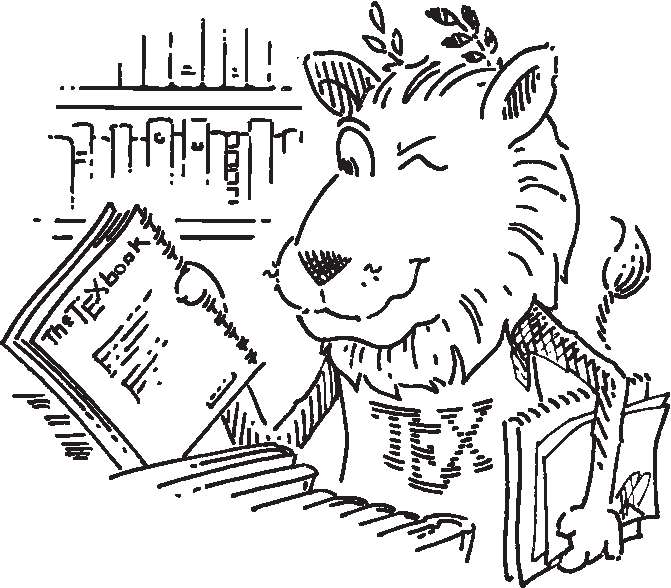
\includegraphics[scale=0.8]{./docs/figs/ctanlion.pdf}
    \end{center}
\vspace{4mm}
\legenda{O mascote do CTAN é um leão originalmente desenhado por Duanne Bibby para o \TeX \textit{book} de \citeonline{knuth/1996} e frequentemente visualizado em outros livros relacionados ao \TeX{} e ao \LaTeX{}.}
\label{fig:leao_ctan}
\FONTE{Adaptado de \url{https://ctan.org/lion/files/ctanlion.eps}.}
\end{figure}

Este material foi escrito com base na experiência pessoal do autor e com base nas necessidades dos alunos da pós-graduação do Instituto Nacional de Pesquisas Espaciais (INPE), compiladas pelo Serviço de Informação e Documentação (SESID) do instituto. A maioria dos exemplos, quando não explicitamente indicada a fonte, é baseada em exemplos pessoais, outros tutoriais sobre a linguagem, \textit{sites} diversos e fóruns como o \TeX{} \textit{Stack Exchange}, além dos manuais e tutoriais do \textit{Overleaf}. Durante a escrita do material, procurou-se organizar as informações de forma que fosse possível ao leitor encontrar o máximo de informações, através dos exemplos e dos resultados em anexo, os quais são mostrados sempre juntos. Uma lista de exercícios também foi incluída para que o leitor possa treinar e adquirir fluência na escrita com a linguagem \LaTeX{}. Devido à grande quantidade de elementos coloridos inseridos ao longo do documento, não recomenda-se a sua impressão. Ao invés disso, orienta-se a utilização desta apostila no computador, de forma que se possa tirar vantagem das ferramentas de busca do visualizador de documentos.

\section{Objetivos}
\label{sec:objetivos}

Nesta apostila são apresentados os conceitos fundamentais da linguagem de marcação \LaTeX{}, com especial atenção à utilização do estilo do INPE para a escrita de dissertações e teses. Os objetivos específicos são:

\begin{itemize}
    \item Apresentar a linguagem de marcação \LaTeX{}, acompanhado de um breve histórico sobre o seu desenvolvimento;
    \item Orientar o usuário sobre a instalação do compilador/interpretador da linguagem nas plataformas mais frequentemente utilizadas;
    \item Expor ao usuário os conceitos fundamentais da linguagem, levando-o a ter independência na utilização do estilo do INPE;
    \item Treinar o usuário na utilização dos estilo do INPE para a escrita de dissertações, teses e propostas.
\end{itemize}

\section{Estrutura e Organização do Documento}
\label{sec:estrutura}

Este documento foi preparado utilizando o estilo de teses e dissertações do INPE, com a finalidade de servir não apenas como uma manual de utilização do estilo, mas também como um documento simples que possa ser utilizado como uma referência no aprendizado da linguagem de marcação \LaTeX{}. Para cumprir com esta finalidade, ao longo dos capítulos e das seções que se seguem, alguns elementos especiais foram incorporados para sinalizar instruções específicas, como comandos do ambiente \textit{Shell} do Linux e dicas ou instruções sobre pontos específicos do que está sendo apresentado. 

Dessa forma, dicas e observações são destacados da seguinte forma:

\begin{marker}
Isto é uma dica ou uma observação!
\end{marker}

De outra forma, comandos que devem ser digitados em um emulador de terminal (e.g., o \textit{Shell} do Linux, Mac OS ou Windows), são destacados como:

\begin{meucomando}
echo ''Isto é um comando de prompt!''
\end{meucomando}

Em geral, estas inserções são mostradas para auxiliar o leitor na execução de comandos que o auxiliarão na instalação de pacotes da linguagem \LaTeX{}, na utilização de \textit{scripts} no \textit{Shell} ou mesmo na utilização de outros programas em linha de comando.

Exemplos da linguagem são apresentados em uma caixa, contendo a grafia dos comandos e o seu resultado em anexo (ao lado ou abaixo). Exercícios são apresentados de forma semelhante, mas com a diferença de que é apresentado um exemplo (e.g., uma tabela) o qual o usuário deverá reproduzir em ambiente local ou \textit{online} configurado para tal. As respostas dos exercícios são então apresentadas no Anexo A. Ao longo do texto, o leitor irá notar que na maioria dos exemplos que contém algum tipo de texto, aparece um texto prolixo. Este texto é gerado automaticamente com o auxílio de um pacote chamado {\tt lipsum}, e não faz, necessariamente, referência a nada específico\footnote{Veja algumas curiosidades sobre este verbete na sua entrada na Wikipedia em \url{https://pt.wikipedia.org/wiki/Lorem_ipsum}.}. Outras frases também utilizadas em alguns exemplos, são ``Jane quer LP, fax, CD, giz, TV e bom whisky'' (um pangrama com 30 letras) e ``À noite, vovô Kowalsky vê o ímã cair no pé do pinguim queixoso e vovó põe açúcar no chá de tâmaras do jabuti feliz'', uma frase com 90 letras, incluindo todas as letras acentuadas. Estas frases foram obtidas da página \url{https://pt.wikipedia.org/wiki/Pangrama}.

O documento está organizado em 4 partes. A Parte \ref{cap:parteI} trata da introdução e objetivos da apostila documento e da linguagem \LaTeX{}. A Parte \ref{cap:parteII} apresenta uma introdução aos elementos e marcadores principais da linguagem. Ao final desta parte, o usuário deverá ser capaz de produzir documentos \LaTeX{} simples, utilizando as classes mais comuns e os elementos textuais mais frequentes. Na Parte \ref{cap:parteIII}, é apresentado o estilo de INPE para a escrita de teses e dissertações. Ao final desta parte, o usuário deverá ser capaz de utilizar o estilo do INPE para a escrita de sua tese ou dissertação. É importante salientar, entretanto, que a Parte \ref{cap:parteIII} requer o aprendizado do conteúdo da Parte \ref{cap:parteII}. A Parte \ref{cap:parteIV}, apresenta o pacote \textit{Beamer}, uma classe que pode ser utilizada para confeccionar apresentações.

\section{Preparação do Ambiente}
\label{sec:prepara}

O \LaTeX{} é um conjunto de \textit{macros} do \TeX{} que são interpretadas por um compilador. Para a sua utilização, é necessário instalar este compilador no computador. Nas seções a seguir, é mostrado como instalar o \LaTeX{} nos sistemas operacionais nos sistemas Windows, Linux e Mac OS. A utilização da linguagem pode ser feita de diversas formas, em linha de comando, utilizando editores de texto puro ou ainda editores mais avançados do tipo \textit{What You See Is What You Get} (WYSIWYG). No entanto, é possível também utilizar a linguagem em editores \textit{online}. A utilização básica da linguagem será vista nos capítulos e seções mais adiante.
 
\subsection{Escolhendo e instalando o compilador}
\label{sec:compilador}

Nas próximas seções, será mostrado como instalar e configurar o compilador/interpretador da linguagem \LaTeX{} nos sistemas operacionais mais utilizados.

\subsection*{Linux}
\label{sec:linux}

Nos sistemas GNU Linux, a instalação do interpretador da linguagem \LaTeX{} e dos seus pacotes é bastante simples, mas pode variar de acordo com a distribuição utilizada. Neste manual, são abordadas as distribuições mais populares e que utilizam os sistemas de pacotes \textit{Advanced Packaging Tool} (APT, para a distribuição Debian e derivados, e.g., Ubuntu e Linux Mint) e \textit{Danified Yum} (DNF, para a distribuição RedHat e derivados, e.g., Fedora e CentOS). A vantagem destes gerenciadores de pacotes está no fato de que eles resolvem automaticamente as dependências, i.e., eles são capazes de instalar outros pacotes que são necessários para o correto funcionamento do programa principal. Em outras distribuições o processo de instalação pode ser diferente ou mesmo envolvendo a instalação a partir dos códigos fonte dos pacotes. 

%O site oficial do \LaTeX{} é o \url{https://www.latex-project.org/}. No Linux, a principal distribuição da linguagem é o pacote \TeX \textit{live} (\url{https://www.tug.org/texlive/}). Para instalar o pacote no Debian e derivados, basta fazer:
No Linux, a principal distribuição da linguagem é o pacote \TeX \textit{live} (\url{https://www.tug.org/texlive/}). Para instalar o pacote no Debian e derivados, basta fazer:

\begin{meucomando}
sudo apt install texlive-full
\end{meucomando}

No RedHat e derivados, basta fazer:

\begin{meucomando}
sudo dnf install texlive-scheme-full
\end{meucomando}

\begin{marker}
Mesmo instalando o pacote completo do ``texlive'', é possível que outros pacotes precisem ser instalados depois.
\end{marker}

Neste momento, pode-se também escolher um editor a fim de que possam ser produzidos documentos localmente. Nesta etapa, sugere-se a instalação do editor \TeX \textit{Studio}:

\begin{meucomando}
sudo apt install texstudio
\end{meucomando}

Analogamente, nas distribuições que utilizam o gerenciados de pacotes DNF:

\begin{meucomando}
sudo dnf install texstudio
\end{meucomando}

\begin{marker}
Para mais detalhes sobre o processo de instalação do \LaTeX{} nas distribuições baseadas no Fedora, acesse a página \url{https://docs.fedoraproject.org/en-US/neurofedora/latex/}. 
\end{marker}

\subsection*{Windows}
\label{sec:windows}

No sistema operacional \textit{Microsoft Windows}, a instalação do pacote \TeX \textit{live} pode ser feita de forma convencional, através do instalador oficial da distribuição disponível em \url{http://mirror.ctan.org/systems/texlive/tlnet/install-tl-windows.exe} (este endereço aponta sempre para o pacote mais recente). Após baixar o pacote, siga as instruções na tela para completar a instalação.

\begin{marker}
O usuário deverá estar atento durante a instalação do \LaTeX{} no Windows, pois o processo de instalação é diferente e pode acarretar em inconvenientes.
\end{marker}

O editor \TeX \textit{Studio} pode ser instalado no \textit{Microsoft Windows} a partir do executável disponível em \url{https://github.com/texstudio-org/texstudio/releases/download/2.12.22/texstudio-2.12.22-win-qt5.exe}.

Outras informações sobre a instalação do \LaTeX{} no sistema operacional \textit{Microsoft Windows}, podem ser encontradas no documento \href{http://mtc-m16d.sid.inpe.br/col/sid.inpe.br/mtc-m19@80/2010/03.24.15.12/doc/ambiente_latex_no_windows.pdf}{oficial} do SESID do INPE.

\subsection*{Mac OS}
\label{sec:macos}

No Mac OS, a forma mais simples de instalar o pacote do \TeX \textit{live} é a partir do instalador disponível em \url{http://tug.org/cgi-bin/mactex-download/MacTeX.pkg} (da mesma forma, este endereço sempre aponta para o pacote mais recente). Se o leitor estiver habituado a utilizar algum tipo de gerenciador de pacote no Mac OS, e.g., o \textit{Homebrew}, orienta-se a utilização deste método para a instalação da distribuição com os seguintes comandos:

\begin{meucomando}
brew install caskroom/cask/brew-cask
brew cask install mactex
\end{meucomando}

\begin{marker}
Se você não possui o gerenciador de pacotes \textit{Homebrew} instalado no seu Mac OS, veja como instalar em \url{https://brew.sh/index_pt-br}.
\end{marker}

Outra forma de instalar os compiladores do \LaTeX{} no Mac OS, é a partir do pacote de instalação do ``MacTeX''. Este pacote pode ser obtido a partir do endereço \url{http://www.tug.org/mactex/mactex-download.html}. Esta é a forma de instalação recomendada para este sistema operacional. Neste pacote estão presentes também alguns programas úteis, como o editor \TeX \textit{Shop}, o gerenciador de referências \textit{BibDesk}, o editor de equações \textit{LaTeXit} e o verificador de gramática \textit{Excalibur}.

Para a edição de documentos \LaTeX{} no Mac OS, recomenda-se também ao leitor a instalação do editor \TeX \textit{Studio}. O instalador deste editor pode ser obtido a partir do endereço \url{https://github.com/texstudio-org/texstudio/releases/}, onde deve ser escolhido o arquivo com a extensão {\tt .dmg}.

Apesar das diferenças entre as instalações do \LaTeX{} com relação aos diferentes sistemas operacionais, os resultados que se obtém a partir da compilação de um documento \LaTeX{} são os mesmos. O leitor deve estar atento também às diferenças entre os tipos de compiladores, cujo uso pode ser diferente. Mais informações sobre os diferentes tipos de compiladores do \LaTeX{}, serão fornecidas nos capítulos e seções a seguir.
 %% 1o capítulo, começo do texto

\chapter{Parte II - Entendendo o \LaTeX{}}
\label{cap:parteII}

\section{Introdução ao \LaTeX{}}
\label{sec:intro_latex}

Com o compilador/interpretador do \LaTeX{} instalado no computador, vamos dar os primeiros passos no aprendizado da linguagem. Vale ressaltar que o objetivo não é aprender ou treinar de forma exaustiva a linguagem, mas levar o leitor a compreender como e quando utilizar a linguagem. Desse forma, nas seções a seguir, são os comandos e estruturas principais da linguagem que são mais frequentemente utilizados em geral.

Antes de iniciarmos com as estruturas textuais, é necessário compreender como a linguagem \LaTeX{} interpreta comandos. A escrita de um documento em linguagem \LaTeX{}, independente do tipo de editor utilizado (e.g., em linha de comando ou um editor do tipo WYSIWYG), o usuário estará sempre escrevendo o código fonte do que virá a ser o seu documento, no formato escolhido com suas tabelas, imagens, equações etc. 

Ao longo das próximas seções, o usuário irá aprender sobre os diversos aspectos da linguagem com vários exemplos, que foram obtidos a partir de várias fontes disponíveis na internet, em fóruns de discussões sobre a linguagem e manuais, disponíveis em diferentes sites. Os exemplos dados são apresentados em caixas destacadas, em que os comando apresentados vem acompanhados dos seus respectivos resultados.

Além disso, ao final do Capítulo \ref{cap:parteII}, há uma série de exercício que o usuário deve realizar a fim de fixar o aprendizado dos comandos aprendidos. Em cada exercício, o usuário deverá reproduzir um exemplo, cujas respostas (comandos \LaTeX{} utilizados) são apropriadamente apresentados em uma seção em anexo ao documento principal.

No trecho de código a seguir é mostrado um documento \LaTeX{}, escrito da forma mais simples:

% Usar os pangramas de https://pt.wikipedia.org/wiki/Pangrama

%\begin{texexptitled}[text only]{Um documento LaTeX mínimo}{exe_doc}
%$\backslash$\mintinline{latex}{documentclass{article}}\\
%$\backslash$\mintinline{latex}{begin{document}}\\
%
%The quick brown fox jumps over the lazy dog.\\
%
%$\backslash$\mintinline{latex}{end{document}}
%\end{texexptitled}

%[breakable,center lower,enhanced,middle=2mm,listing side text]
%\begin{texexptitled}[breakable,center lower,enhanced jigsaw,middle=2mm,listing side comment,righthand width=6cm,compilable listing,run latex,run dvips,run ps2pdf,pdf comment,freeze pdf,comment style={raster columns=1}]{Um documento LaTeX mínimo}{exe_doc}
\begin{texexptitled}[breakable,center lower,enhanced jigsaw,middle=2mm,listing side comment,righthand width=6cm,compilable listing,run latex,run dvips,run ps2pdf,pdf comment,freeze pdf,comment style={raster columns=1}]{Um documento \LaTeX{} mínimo}{exe_doc}
\documentclass{article}
\usepackage[utf8]{inputenc}

\title{Um Documento \LaTeX{} mínimo utilizando a classe {\tt article}}
\author{Carlos Frederico Bastarz}
\date{September 2019}

\begin{document}

\maketitle

\section{Seção}

\lipsum[1]

\subsection{Subseção}

\lipsum[2]

\end{document}
\end{texexptitled}

%%[breakable,center lower,enhanced,middle=2mm,listing side text]
%\begin{tcblisting}{enhanced jigsaw,
%title={Um documento LaTeX mínimo},
%fonttitle=\small\sffamily\bfseries,
%colframe=MaterialBlue900,
%colback=white,
%listing options={
%style=tcblatex,
%texcsstyle=*\color{red!70!black}},
%lower separated=false,
%middle=2mm,
%listing side comment,
%righthand width=6cm,
%compilable listing,
%run latex,run dvips,run ps2pdf,pdf comment,freeze pdf,
%comment style={raster columns=1},%,graphics options={viewport=0.25in 3.7in 1.5in 5.5in}},
%}
%\documentclass{article}
%\usepackage[utf8]{inputenc}
%\usepackage{lipsum}
%
%\title{Um Documento LaTeX mínimo utilizando a classe {\tt article}}
%\author{Carlos Frederico Bastarz}
%\date{September 2019}
%
%\begin{document}
%
%\maketitle
%
%\section{Introdução}
%\lipsum[1]
%
%\subsection{Desenvolvimento}
%\lipsum[2]
%
%\subsection{Conclusão}
%\lipsum[3]
%
%\end{document}
%\end{tcblisting}

% TEXTO EM DUAS COLUNAS

%\begin{texexptitled}[listing and comment,righthand width=3cm,lower separated=false,middle=1mm,pdf comment={./snippets/teste_merge.pdf},comment style={raster columns=4,graphics pages={1,2,3,4,5,6,7,8,10,11,12,13},colframe=blue,drop fuzzy shadow}]{Um documento LaTeX mínimo}{exe_doc}
%$\backslash$\mintinline{latex}{documentclass{article}}\\
%$\backslash$\mintinline{latex}{begin{document}}\\
%
%The quick brown fox jumps over the lazy dog.\\
%
%$\backslash$\mintinline{latex}{end{document}}
%\end{texexptitled}

%% \tcbuselibrary{skins,raster}
%\begin{tcblisting}{colback=red!5!white,colframe=red!75!black,listing and comment,
%righthand width=3cm,lower separated=false,middle=1mm,
%pdf comment={./snippets/teste1.pdf},
%comment style={raster columns=3,graphics pages={1,2,3},
%colframe=blue,drop fuzzy shadow}}
%This is a \LaTeX\ example.
%\end{tcblisting}

No Exemplo \ref{exe_doc} acima, observe que um documento \LaTeX{} possui uma estrutura específica que se inicia com um descrição do tipo de documento dado pelo comando \mintinline{latex}{documentclass} (indicando que o documento tem o formato de \textit{article}, i.e., um artigo). Tudo o que é escrito entre esta instrução e a próxima ({\tt document}), é chamada de ``preâmbulo''. Nesta seção podem ser carregados pacotes específicos da linguagem que permitem o uso de diferentes ambientes além de outros tipos de marcação. Em seguida, inicia-se o ambiente principal do \LaTeX{}, que é o \mintinline{latex}{document}. Entre as palavras reservadas \mintinline{latex}{begin} e \mintinline{latex}{end}, o documento em si é escrito. Documentos \LaTeX{}, independente da sua classe (que pode ser \textit{book}, \textit{report}, \textit{article} e \textit{letter}), podem ser muito simples ou complexos. O estilo para Teses e Dissertações do INPE (apresentado no Capítulo \ref{cap:parteIII}), é um exemplo de documento complexo que inclui estilo e formatação próprios.

\begin{marker}
  Na \textit{internet} é muito comum encontrar exemplos simplificados de documentos. Ao procurar por estes exemplos em inglês, utilize a palavra-chave \textit{Minimal Working Example} ou MWE.
\end{marker}

%% CRIAR UM SNIPPET E USAR O EXEMPLO ABAIXO
%\begin{listing}[ht]
%\inputminted{octave}{BitXorMatrix.m}
%\caption{Example from external file}
%\label{listing:3}
%\end{listing}

Nas próximas seções, iremos tratar dos diversos marcadores que podem ser utilizados para alterar a aparência e o posicionamento dos textos e parágrafos.

\subsection{Caracteres e símbolos especiais}
\label{sec:carac_especiais}

No \LaTeX{} há 10 tipos de caracteres especiais. São eles:

\begin{multicols}{5}
    \begin{enumerate}
        \item $\backslash$
        \item \#
        \item \$
        \item \%
        \item \&
        \item \^{}
        \item \_
        \item \{
        \item \}
        \item \texttt{\~{}}
    \end{enumerate}
\end{multicols}

% FALTA: ACENTOS

Às vezes é necessários utilizá-los ao longo do texto, e então, faz necessário ``escapá-los''. Há duas formas de fazer isso. 1) Escapando-os ou; 2) Utilizando comandos especiais.

Na primeira forma, basta utilizar a barra invertida ``$\backslash\backslash$''. Na segunda, pode-se utilizar comandos específicos do \LaTeX{}. 

%Exemplos:
%
%\begin{minipage}{0.5\linewidth}
%    \begin{comando}{Comando}
%        \begin{center}
%            \mintinline{latex}{\textbackslash{}} \\
%            \mintinline{latex}{\^{} ou \textasciicircum{}} \\
%            \mintinline{latex}{\~{} ou \textasciitilde{}}
%        \end{center}
%    \end{comando}
%\end{minipage}
%\begin{minipage}{0.5\linewidth}
%    \begin{resultado}{Resultado}
%        \begin{center}
%            $\backslash$ \\
%            \^{} \\
%            \texttt{\~{}}
%        \end{center}
%    \end{resultado}
%\end{minipage}

\begin{texexptitled}[breakable,center lower,enhanced,middle=2mm,listing side text]{Marcação para caracteres especiais}{exe_caracesp}
$\backslash$ \\
\^{} \\
\texttt{\~{}}
\end{texexptitled}

\begin{marker}
  No Exemplo \ref{exe_caracesp}, o marcador \mintinline{latex}{\\} pula uma linha. Pode-se também utilizar o comando \mintinline{latex}{\newline}.
\end{marker}

\subsection{Acentos}
\label{sec:acentos}

No \LaTeX{}, os acentos podem ser escritos de forma literal, i.e., diretamente nas palavras sem a necessidade de marcadores especiais, desde que os pacotes necessários estejam carregados. O \textit{babel} é um pacote do \LaTeX{} que fornece os formatos de marcação e linguagem adequados para a acentuação de, por exemplo, caracteres latinos acentuados. Para digitar acentos de forma natural, é necessário carregar os pacotes a seguir, no preâmbulo do documento:

\begin{itemize}
    \item \mintinline{latex}{\usepackage[brazilian]{babel}}
    \item \mintinline{latex}{\usepackage[utf8]{inputenc}}
    \item \mintinline{latex}{\usepackage[T1]{fontenc}}
\end{itemize}

\begin{marker}
  No estilo do INPE, os pacotes relacionados acima já estão pré-carregados. Porém, se o usuário utilizar o compilador \XeLaTeX{}, encontrará erros enquanto o pacote estiver carregado.
\end{marker}

Entretanto, em algumas situações é necessário marcar-se os acentos de forma explícita (e.g., na edição de um arquivo de referências do BibTeX).

No Exemplo \ref{exe_acentos} a seguir, são mostrados os acentos mais comuns.

\begin{texexptitled}[breakable,center lower,enhanced,middle=2mm,listing side text]{Uso de acentos latinos no \LaTeX{}}{exe_acentos}
\'a \'A \'e \'E \'i \'I \'o \'O \'u \'U
\\
\^a \^A \~a \~A \`a \`A \~o \~O
\\
\^e \^E \^o \^O
\\
\"u \"U
\\
\c{c} \c{C}
\end{texexptitled}

\begin{marker}
  Outras marcações especiais para acentuação de caracteres podem ser obtidas em \url{https://en.wikibooks.org/wiki/LaTeX/Special_Characters}.
\end{marker}

\subsection{Tipos, tamanhos e estilos de letras}
\label{sec:marc_text}

O texto básico pode ser marcado em estilos comuns, como o \textit{itálico}, o \underline{sublinhado}, o \textbf{negrito}, o texto \textsuperscript{sobrescrito} e o texto \textsubscript{subscrito}. 

\begin{texexptitled}[breakable,center lower,enhanced,middle=2mm,listing side text]{Estilos mais comuns em fontes}{exe_estilos}
\textit{itálico} \\
\textsl{itálico} \\
\underline{sublinhado} \\
\textbf{negrito} \\
\textsuperscript{o}C \\
H\textsubscript{2}O
\end{texexptitled}

No Exemplo \ref{exe_estilos}, observe as diferenças entre o texto itálico produzido com o marcador \mintinline{latex}{\textit} e o texto inclinado produzido pelo marcador \mintinline{latex}{\textsl{}}. No primeiro caso, as fontes produzidas são naturais, ou seja, há uma variação em itálico do tipo de fonte original. No segundo caso, a fonte original é renderizada a partir da inclinação da fonte natural. 
\begin{marker}
Dependendo do tipo de fonte utilizado, as diferenças entre os tipos itálico e inclinado podem ser mais evidentes. Veja mais no Exemplo \ref{exe_font}.
\end{marker}

Outros estilos também podem ser utilizados, mas dependem de outros pacotes. Dois pacotes que fornecem estilos de marcações sobre as palavras, são o \mintinline{latex}{ulem} e o \mintinline{latex}{cancel}. Para utilizá-los, deve-se antes carregar os pacotes necessários com os comandos \mintinline{latex}{\usepackage{ulem}} e \mintinline{latex}{\usepackage{cancel}}. 

Com o pacote \mintinline{latex}{ulem}, pode-se riscar as palavras (forma mais comum).

\begin{texexptitled}[breakable,center lower,enhanced,middle=2mm,listing side text]{Marcação com o pacote \mintinline{latex}{ulem}}{exe_ulem}
\sout{palavra riscada}
\end{texexptitled}

% ARRUMAR O EXEMPLO ABAIXO, COLOCANDO EXPRESSÕES MATEMÁTICAS
\begin{texexptitled}[breakable,center lower,enhanced,middle=2mm,listing side text]{Marcação com o pacote \mintinline{latex}{cancel}}{exe_cancel}
$\cancel{palavra cancelada}$
$\bcancel{palavra cancelada}$
$\xcancel{palavra cancelada}$
$\cancelto{valor}{expressao}$
\end{texexptitled}

No \LaTeX{}, ao longo de um parágrafo, é possível alterar o tamanho da fonte. Por padrão há 10 tamanhos de letra que podem ser utilizados.

\begin{texexptitled}[breakable,center lower,enhanced,middle=2mm,listing side text]{Tamanhos de fontes}{exe_tamfonte}
\Huge Huge \\
\huge huge \\
\LARGE LARGE \\
\Large Large \\
\large large \\
\normalsize normalsize \\
\small small \\
\footnotesize footnotesize \\
\scriptsize scriptsize \\
\tiny tiny
\end{texexptitled}

Para alterar o tamanho de uma fonte localmente, basta fazer \mintinline{latex}{\large large}.

No \LaTeX{} é possível também alterar o tipo da fonte. Alguns estilos incluem fontes no estilo \mintinline{latex}{\texttt{}} (máquina de escrever), \mintinline{latex}{\textsf{}} (com serifa) e \mintinline{latex}{\textrm{}} (sem serifa).

\begin{texexptitled}[breakable,center lower,enhanced,middle=2mm]{Alguns tipos de fontes}{exe_font}
\texttt{Typewriter Font} | 
\texttt{\textit{Typewriter Font}} |
\texttt{\textsl{Typewriter Font}}

\textsf{Serif Font} | 
\textsf{\textit{Serif Font}} | 
\textsf{\textsl{Serif Font}}

\textrm{Roman Font} | 
\textrm{\textit{Roman Font}} | 
\textrm{\textsl{Roman Font}}
\end{texexptitled}

\subsection{Títulos e seções}
\label{sec:tit_secs}

No \LaTeX{}, é possível organizar o texto utilizando seções em até 7 níveis.

% Dica dos expaçamentos: https://tex.stackexchange.com/questions/10535/how-to-force-a-table-into-page-width/56552
\begin{table}[ht]
\caption{Títulos e Seções de um documento \LaTeX{}.}
\begin{center}
    \begin{tabular}{p{5cm}p{5cm}c}
    \hline
    \\[-0.5em]
    \textbf{Seção} & \textbf{Comando}              & \textbf{Nível} \\
    \\[-0.5em]
    \hline
    \hline
    \\[-0.5em]
    Parte        & \mintinline{latex}{\part}       & -1    \\
    \\[-0.5em]
    Capítulo     & \mintinline{latex}{\chapter}    & 0     \\
    \\[-0.5em]
    Seção        & \mintinline{latex}{\section}    & 1     \\
    \\[-0.5em]
    Subseção     & \mintinline{latex}{\subsection} & 2     \\
    \\[-0.5em]
    Parágrafo    & \mintinline{latex}{\par}        & 3     \\
    \\[-0.5em]
    Subparágrafo & \mintinline{latex}{\subpar}     & 4     \\
    \\[-0.5em]
    \hline
    \end{tabular}
\end{center}
\label{tab:tit_secs}
\end{table}

Na Seção \ref{sec:intro_latex} foram mostradas as diferentes classes padrão disponíveis para documentos \LaTeX{}. Observe que as partes de conteúdo marcadas como \mintinline{latex}{\part} e \mintinline{latex}{chapter} estão disponíveis apenas para as classes \mintinline{latex}{report} e \mintinline{latex}{book}.

\subsection{Cores e Paletas de Cores}
\label{sec:pal_cores}

% REF: https://martin-thoma.com/colors-in-latex/
%A paleta de cores padrão do LaTeX pode ser alterada.
As cores padrão que geralmente são utilizadas em um documento,  e que não dependem de pacotes extras, são apresentadas a seguir.

%%\begin{texexptitled}[breakable,center lower,enhanced,middle=2mm]{Texto colorido}{exe_cor2}
\begin{center}
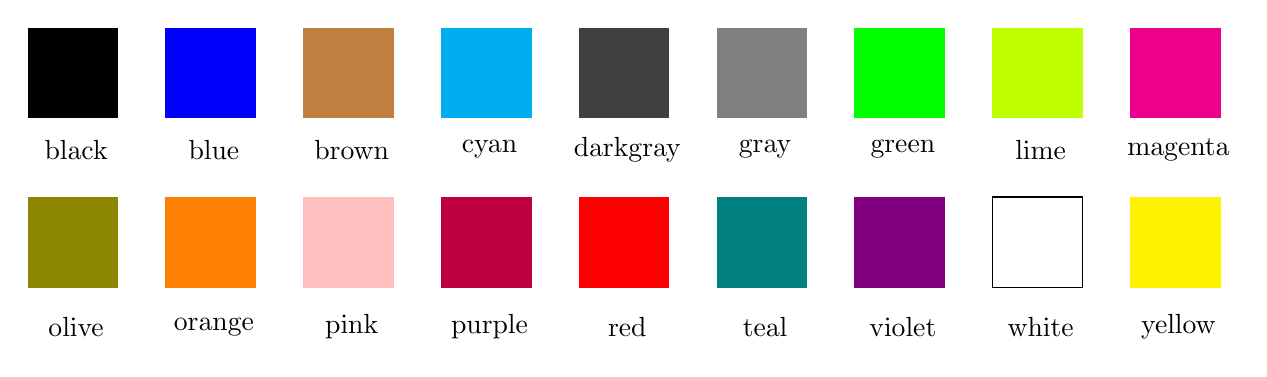
\begin{tikzpicture}
\fill [black] (0,0) rectangle ++(1.15,1.15);
\draw (0.615,-0.4) node {black};
\fill [blue] (1.75,0) rectangle ++(1.15,1.15);
\draw (2.365,-0.4) node {blue};
\fill [brown] (3.5,0) rectangle ++(1.15,1.15);
\draw (4.115,-0.4) node {brown};
\fill [cyan] (5.25,0) rectangle ++(1.15,1.15);
\draw (5.865,-0.4) node {cyan};
\fill [darkgray] (7,0) rectangle ++(1.15,1.15);
\draw (7.615,-0.4) node {darkgray};
\fill [gray] (8.75,0) rectangle ++(1.15,1.15);
\draw (9.365,-0.4) node {gray};
\fill [green] (10.5,0) rectangle ++(1.15,1.15);
\draw (11.115,-0.4) node {green};
\fill [lime] (12.25,0) rectangle ++(1.15,1.15);
\draw (12.865,-0.4) node {lime};
\fill [magenta] (14,0) rectangle ++(1.15,1.15);
\draw (14.615,-0.4) node {magenta};

\fill [olive] (0,-1) rectangle ++(1.15,-1.15);
\draw (0.615,-2.65) node {olive};
\fill [orange] (1.75,-1) rectangle ++(1.15,-1.15);
\draw (2.365,-2.65) node {orange};
\fill [pink] (3.5,-1) rectangle ++(1.15,-1.15);
\draw (4.115,-2.65) node {pink};
\fill [purple] (5.25,-1) rectangle ++(1.15,-1.15);
\draw (5.865,-2.65) node {purple};
\fill [red] (7,-1) rectangle ++(1.15,-1.15);
\draw (7.615,-2.65) node {red};
\fill [teal] (8.75,-1) rectangle ++(1.15,-1.15);
\draw (9.365,-2.65) node {teal};
\fill [violet] (10.5,-1) rectangle ++(1.15,-1.15);
\draw (11.115,-2.65) node {violet};
\draw[fill=white] (12.25,-1) rectangle ++(1.15,-1.15);
\draw (12.865,-2.65) node {white};
\fill [yellow] (14,-1) rectangle ++(1.15,-1.15);
\draw (14.615,-2.65) node {yellow};
\end{tikzpicture}
%%\end{texexptitled}
\end{center}

Assim como em qualquer editor de textos WYSIWYG, as cores do texto podem ser alteradas para palavras isoladas, frases ou parágrafos.

\begin{texexptitled}[breakable,center lower,enhanced,middle=2mm]{Texto com fonte colorida}{exe_cor1}
\textit{The \color{pink}{quick} \color{magenta}{brown} fox jumps \color{green}{over} the lazy \color{blue}{dog}.}
\end{texexptitled}

Além de modificar a cor das fontes, é possível também marcá-las de forma que o fundo fique colorido.

\begin{texexptitled}[breakable,center lower,enhanced,middle=2mm]{Texto com fundo colorido}{exe_cor3}
\textit{The \colorbox{pink}{quick} \colorbox{magenta}{brown} fox jumps \colorbox{green}{over} the lazy \colorbox{blue}{\color{white}{dog}}.}
\end{texexptitled}

Você pode escolher, por exemplo, utilizar a patela de cores do projeto ``Solarized''. Para utilizá-la, basta carregar o pacote \mintinline{latex}{\usepackage{solarized}}. A paleta de cores do ``Solarized'' é a seguinte:

%\begin{center}
%\solarizedPalette
%\end{center}

\begin{center}
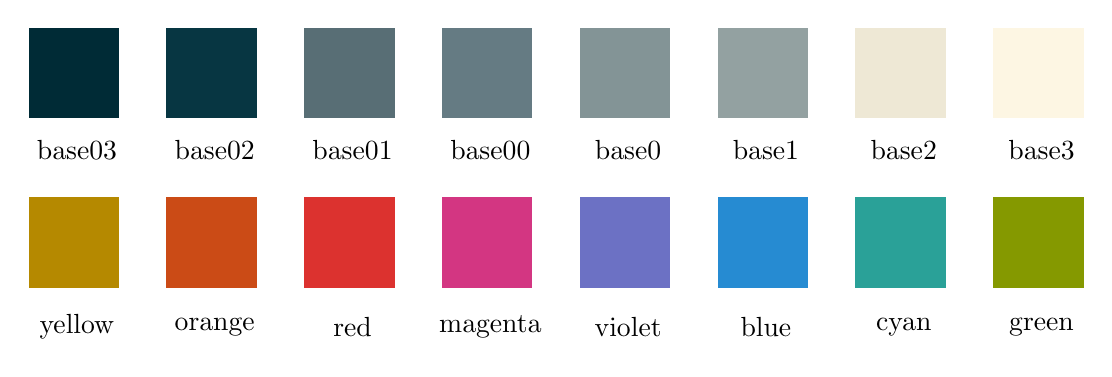
\begin{tikzpicture}
\fill [solarized-base03] (0,0) rectangle ++(1.15,1.15);
\draw (0.615,-0.4) node {base03};
\fill [solarized-base02] (1.75,0) rectangle ++(1.15,1.15);
\draw (2.365,-0.4) node {base02};
\fill [solarized-base01] (3.5,0) rectangle ++(1.15,1.15);
\draw (4.115,-0.4) node {base01};
\fill [solarized-base00] (5.25,0) rectangle ++(1.15,1.15);
\draw (5.865,-0.4) node {base00};
\fill [solarized-base0] (7,0) rectangle ++(1.15,1.15);
\draw (7.615,-0.4) node {base0};
\fill [solarized-base1] (8.75,0) rectangle ++(1.15,1.15);
\draw (9.365,-0.4) node {base1};
\fill [solarized-base2] (10.5,0) rectangle ++(1.15,1.15);
\draw (11.115,-0.4) node {base2};
\fill [solarized-base3] (12.25,0) rectangle ++(1.15,1.15);
\draw (12.865,-0.4) node {base3};
%\fill [solarized-] (14,0) rectangle ++(1.15,1.15);
%\draw (14.615,-0.4) node {teal};

\fill [solarized-yellow] (0,-1) rectangle ++(1.15,-1.15);
\draw (0.615,-2.65) node {yellow};
\fill [solarized-orange] (1.75,-1) rectangle ++(1.15,-1.15);
\draw (2.365,-2.65) node {orange};
\fill [solarized-red] (3.5,-1) rectangle ++(1.15,-1.15);
\draw (4.115,-2.65) node {red};
\fill [solarized-magenta] (5.25,-1) rectangle ++(1.15,-1.15);
\draw (5.865,-2.65) node {magenta};
\fill [solarized-violet] (7,-1) rectangle ++(1.15,-1.15);
\draw (7.615,-2.65) node {violet};
\fill [solarized-blue] (8.75,-1) rectangle ++(1.15,-1.15);
\draw (9.365,-2.65) node {blue};
\fill [solarized-cyan] (10.5,-1) rectangle ++(1.15,-1.15);
\draw (11.115,-2.65) node {cyan};
\fill [solarized-green] (12.25,-1) rectangle ++(1.15,-1.15);
\draw (12.865,-2.65) node {green};
%\fill [solarized-] (14,-1) rectangle ++(1.15,-1.15);
%\draw (14.615,-2.65) node {grey};
\end{tikzpicture}
\end{center}

Para utilizar as novas cores, basta utilizar um dos nomes definidos pela paleta, precedido por \mintinline{latex}{solarized-}. Por exemplo: \mintinline{latex}{solarized-red}.

Outra paleta de cores armoniozas, é provido pelo pacote {\tt xcolor-material}. Esta é a paleta de cores do \textit{Material Design} do Google. Para utilizá-la, basta carregar o pacote \mintinline{latex}{\usepackage{xcolor-material}} no preâmbulo do documento. 

As cores básicas do pacote {xcolor-material} são as seguintes (além do branco e preto):

\begin{center}
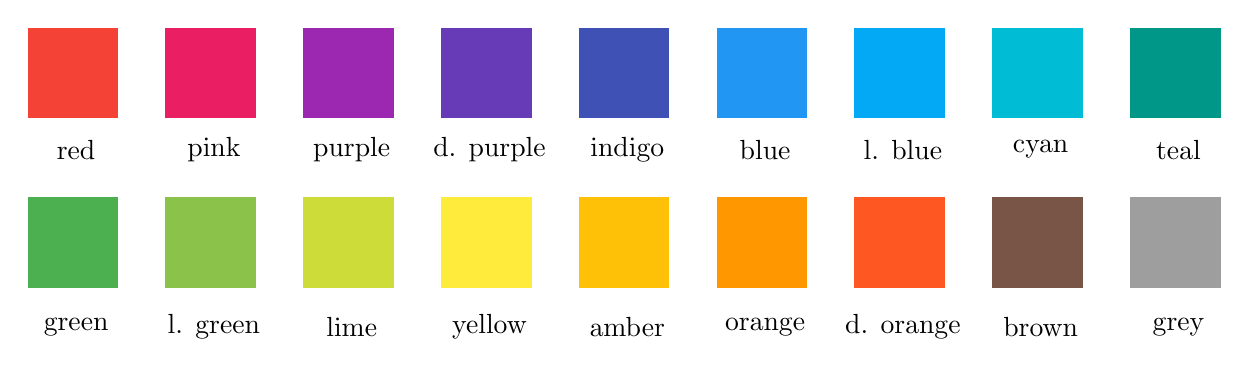
\begin{tikzpicture}
\fill [MaterialRed] (0,0) rectangle ++(1.15,1.15);
\draw (0.615,-0.4) node {red};
\fill [MaterialPink] (1.75,0) rectangle ++(1.15,1.15);
\draw (2.365,-0.4) node {pink};
\fill [MaterialPurple] (3.5,0) rectangle ++(1.15,1.15);
\draw (4.115,-0.4) node {purple};
\fill [MaterialDeepPurple] (5.25,0) rectangle ++(1.15,1.15);
\draw (5.865,-0.4) node {d. purple};
\fill [MaterialIndigo] (7,0) rectangle ++(1.15,1.15);
\draw (7.615,-0.4) node {indigo};
\fill [MaterialBlue] (8.75,0) rectangle ++(1.15,1.15);
\draw (9.365,-0.4) node {blue};
\fill [MaterialLightBlue] (10.5,0) rectangle ++(1.15,1.15);
\draw (11.115,-0.4) node {l. blue};
\fill [MaterialCyan] (12.25,0) rectangle ++(1.15,1.15);
\draw (12.865,-0.4) node {cyan};
\fill [MaterialTeal] (14,0) rectangle ++(1.15,1.15);
\draw (14.615,-0.4) node {teal};

\fill [MaterialGreen] (0,-1) rectangle ++(1.15,-1.15);
\draw (0.615,-2.65) node {green};
\fill [MaterialLightGreen] (1.75,-1) rectangle ++(1.15,-1.15);
\draw (2.365,-2.65) node {l. green};
\fill [MaterialLime] (3.5,-1) rectangle ++(1.15,-1.15);
\draw (4.115,-2.65) node {lime};
\fill [MaterialYellow] (5.25,-1) rectangle ++(1.15,-1.15);
\draw (5.865,-2.65) node {yellow};
\fill [MaterialAmber] (7,-1) rectangle ++(1.15,-1.15);
\draw (7.615,-2.65) node {amber};
\fill [MaterialOrange] (8.75,-1) rectangle ++(1.15,-1.15);
\draw (9.365,-2.65) node {orange};
\fill [MaterialDeepOrange] (10.5,-1) rectangle ++(1.15,-1.15);
\draw (11.115,-2.65) node {d. orange};
\fill [MaterialBrown] (12.25,-1) rectangle ++(1.15,-1.15);
\draw (12.865,-2.65) node {brown};
\fill [MaterialGrey] (14,-1) rectangle ++(1.15,-1.15);
\draw (14.615,-2.65) node {grey};
\end{tikzpicture}
\end{center}

Na paleta de cores mostrada acima, ``d.'' foi utilizado para abreviar a palavra \textit{deep} e ``l.'' foi utilizada para abreviar a palavra \textit{light}. Para utilizar as cores do pacote {\tt xcolor-material}, é necessário utilizá-las da seguinte forma: a cor \textit{Deep Purple} deve ser referenciada como ``MaterialDeepPurple'', ou seja, a palavra reservada ``Material'' deve preceder o nome da cor, que por sua vez, deve ser indicada com a primeira letra em caixa alta.

\begin{marker}
  Pode ser necessário incluir o arquivo {\tt xcolor-material.sty} à sua distribuição \LaTeX{}. Veja a página do pacote para mais informações (\url{https://www.ctan.org/pkg/xcolor-material}).
\end{marker}

Se for necessário, é possível definir qualquer cor utilizando códigos HTML, \textit{Red Green Blue} (RGB) ou \textit{Cyan Magenta Yellow Black} (CMYK) utilizando o comando \mintinline{latex}{\definecolor}.

\begin{texexptitled}[breakable,center lower,enhanced,middle=2mm]{Definindo cores}{exe_cor4}
\definecolor{meularanja1}{HTML}{FF7F00}
\definecolor{meularanja2}{rgb}{1,0.5,0}
\definecolor{meularanja3}{RGB}{255,127,0}
\definecolor{meularanja4}{cmyk}{0,0.5,1,0}

\begin{tikzpicture}
\fill [meularanja1] (0,0) rectangle ++(1.25,1.25);
\draw (0.6,-0.5) node {meularanja1};
\fill [meularanja2] (3,0) rectangle ++(1.25,1.25);
\draw (3.6,-0.5) node {meularanja2};
\fill [meularanja3] (6,0) rectangle ++(1.25,1.25);
\draw (6.6,-0.5) node {meularanja3};
\fill [meularanja4] (9,0) rectangle ++(1.25,1.25);
\draw (9.6,-0.5) node {meularanja4};
\end{tikzpicture}
\end{texexptitled}

\begin{marker}
Veja outras opções de paletas e cores em \href{http://latexcolor.com}{LaTeXColor}.
\end{marker}

\subsection{Medidas}
\label{sec:medidas}

As medidas na linguagem \LaTeX{} podem ser apresentadas em unidades diversas. Você pode misturá-las e isso pode ocorrer quando você reutiliza algum código que produz uma formatação específica que você gostaria de criar e acabou encontrando na internet. A Tabela \ref{tab:medidas} a seguir, mostra as unidades mais comuns. Vale ressaltar, entretanto, que a unidade padrão é o ponto e que o comprimento padrão é \mintinline{latex}{1 pt}:

\begin{table}[H]
\centering
\caption{Unidades de Medidas mais Comuns no \LaTeX{}.}
\label{tab:medidas}
%\begin{center}
    \begin{tabular}{p{3cm}cc}
    \hline
    \\[-0.5em]
    \textbf{Abreviação} & \textbf{Definição} & \textbf{Valor em Pontos} \\
    \\[-0.5em]
    \hline
    \hline
    \\[-0.5em]
    Ponto           & \mintinline{latex}{pt} & $1$                              \\
    \\[-0.5em]
    Milímetro       & \mintinline{latex}{mm} & $2,84$ = $\frac{7227}{2540}$     \\
    \\[-0.5em]
    Centímetro      & \mintinline{latex}{cm} & $28,4$ = $\frac{7227}{254}$      \\
    \\[-0.5em]
    Polegada        & \mintinline{latex}{in} & $72,27$     \\
    \\[-0.5em]
    Altura de ``x'' & \mintinline{latex}{ex} & \textit{Depende da fonte utilizada} \\
    \\[-0.5em]
    Altura de ``M'' & \mintinline{latex}{em} & \textit{Depende da fonte utilizada} \\
    \\[-0.5em]
    \hline
    \end{tabular}
%\end{center}
%\label{tab:medidas}
\end{table}

Em documentos escritos na linguagem \LaTeX{}, é possível especificar as medidas utilizando os valores nas unidades indicadas na tabela acima e também utilizando algumas macros. Estas macros são, especificamente, representam algumas medidas padrão na linguagem e são apresentadas na Tabela \ref{tab:meds_padrao} abaixo.

\begin{table}[H]
\centering
\caption{Algumas Macros de Medidas do \LaTeX{}.}
\label{tab:meds_padrao}
    \begin{tabular}{p{5cm}p{8cm}}
    \hline
    \\[-0.5em]
    \textbf{Macro} & \textbf{Descrição} \\
    \\[-0.5em]
    \hline
    \hline
    \\[-0.5em]
    \mintinline{latex}{\baselineskip}    & Distância vertical entre as linhas em um parágrafo \\
    \\[-0.5em]
    \mintinline{latex}{\baselinestretch} & Fator para ser utilizado com o marcador \mintinline{latex}{\baselineskip} (exemplo: \mintinline{latex}{\renewcommand{\baselinestretch}{fator}}) \\
    \\[-0.5em]
    \mintinline{latex}{\columnsep}       & Distância entre colunas \\
    \\[-0.5em]
    \mintinline{latex}{\columnwidth}     &  Largura de uma coluna \\
    \\[-0.5em]
    \mintinline{latex}{\evensidemargin}  & Margens em páginas `pares' \\
    \\[-0.5em]
    \mintinline{latex}{\linewidth}       & Largura de uma linha em um ambiente local \\
    \\[-0.5em]
    \mintinline{latex}{\oddsidemargin}   & Margens em páginas `ímpares' \\
    \\[-0.5em]
    \mintinline{latex}{\paperwidth}      & Largura de uma página \\
    \\[-0.5em]
    \mintinline{latex}{\paperheight}     & Altura de uma página \\
    \\[-0.5em]
    \mintinline{latex}{\parindent}       & Indentação de um parágrafo \\
    \\[-0.5em]
    \mintinline{latex}{\parskip}         & Espaçamento extra entre parágrafos \\
    \\[-0.5em]
    \mintinline{latex}{\tabcolsep}       & Separação normal entre as colunas no ambiente \mintinline{latex}{\tabular} \\
    \\[-0.5em]
    \mintinline{latex}{\textheight}      & Altura do texto na página \\
    \\[-0.5em]
    \mintinline{latex}{\textwidth}       & Largura do texto na página \\
    \\[-0.5em]
    \mintinline{latex}{\topmargin}       & Tamanho da margem de cima \\
    \\[-0.5em]
    \mintinline{latex}{\unitlength}      & Unidades de comprimento no ambiente \mintinline{latex}{\picture} \\
    \\[-0.5em]
    \hline
    \end{tabular}
\end{table}

No \LaTeX{}, um comprimento é um número real seguido por uma unidade de media, o qual pode ser modificado por um valor ou uma macro. 

Além de medidas padrão, o \LaTeX{} também fornece macros que permitem adicionar espaçamentos (horizontais e verticais), que podem fazer uso das medidas relacionadas na Tabela \ref{tab:meds_padrao}. Veja a Tabela \ref{tab:espacamentos} a seguir:

\begin{table}[H]
\centering
\caption{Algumas Macros de Espaçamento do \LaTeX{}.}
\label{tab:espacamentos}
    \begin{tabular}{p{5cm}p{8cm}}
    \hline
    \\[-0.5em]
    \textbf{Macro} & \textbf{Descrição} \\
    \\[-0.5em]
    \hline
    \hline
    \\[-0.5em]
    \mintinline{latex}{\hspace}          & Adiciona espaço horizontal (pode utilizar qualquer unidade da Tabela \ref{tab:medidas}, incluindo valores negativos) \\
    \\[-0.5em]
    \mintinline{latex}{\vspace}          & Adiciona espaço vertical (pode utilizar qualquer unidade da Tabela \ref{tab:medidas}, incluindo valores negativos)\\
    \\[-0.5em]
    \mintinline{latex}{\smallskip}       & Equivalente a \mintinline{latex}{\vspace{smallskipamount}}, onde {\tt smallskipamount} é relativo ao estilo do documento \\
    \\[-0.5em]
    \mintinline{latex}{\medskip}         & Equivalente a \mintinline{latex}{\vspace{medskipamount}}, onde {\tt medskipamount} é relativo ao estilo do documento \\
    \\[-0.5em]
    \mintinline{latex}{\bigskip}         & Equivalente a \mintinline{latex}{\vspace{bigskipamount}}, onde {\tt bigskipamount} é relativo ao estilo do documento \\
    \\[-0.5em]
    \hline
    \end{tabular}
\end{table}

%% INCLUIR ALGUNS EXEMPLOS DE USO DOS COMANDOS DA TABELA ACIMA.

%\begin{texexptitled}{Comprimento modificado por um valor \mintinline{latex}{50.5pt plus 1pt minus 2pt}}{exe_medidas1}
%\setlength{\parindent}{0em}
%\lipsum[1]
%\setlength{\parindent}{50.5pt plus 1pt minus 2pt}
%\lipsum[2]
%\end{texexptitled}
%
%\begin{texexptitled}{Comprimento modificado por uma macro \mintinline{latex}{10\textwidth}}{exe_medidas2}
%\setlength{\parindent}{0em}
%\lipsum[1]
%\setlength{\parindent}{10\textwidth}
%\lipsum[2]
%\end{texexptitled}

\begin{marker}
Veja mais detalhes, informações e exemplos em \url{https://en.wikibooks.org/wiki/LaTeX/Lengths}.
\end{marker}

\subsection{Parágrafos}
\label{sec:paragrafos}

Os parágrafos no \LaTeX{} são blocos de texto separados por uma ou mais linhas. Para iniciar um parágrafo, basta pular uma linha. Uma outra forma de separar parágrafos, é através da utilização de duas barras invertidas (\mintinline{latex}{\\}). Observe as diferenças entre os exemplos a seguir.

\begin{texexptitled}[breakable,enhanced,middle=2mm]{Parágrafos Contíguos}{exe_par1}
\lipsumsentence[1-4] 
\lipsumsentence[5-8]
\end{texexptitled}

\begin{texexptitled}[breakable,enhanced,middle=2mm]{Parágrafos Separados por um Espaço}{exe_par2}
\lipsumsentence[1-4]  

\lipsumsentence[5-8]
\end{texexptitled}

\begin{texexptitled}[breakable,enhanced,middle=2mm]{Parágrafos Separados por Duas Barras invertidas (\mintinline{latex}{\\})}{exe_par3}
\lipsumsentence[1-4] \\ 
\lipsumsentence[5-8]
\end{texexptitled}

\subsubsection*{Posição e espaçamento}
\label{sec:pos_espac}

Boa parte dos elementos de um texto podem ser, basicamente, posicionados à esquerda, ao centro ou à direita. O \LaTeX{} possui marcadores especiais para estes posicionamentos, que podem ser utilizados não apenas nos parágrafos, mas também com figuras e tabelas.

\begin{texexptitled}[breakable,enhanced,middle=2mm]{Parágrafos centralizados \par Utilizando o ambiente \mintinline{latex}{center}}{exe_par4}
\begin{center}
\lipsumsentence[9-10] \\ 
\lipsumsentence[11-12]
\end{center}
\end{texexptitled}

Além de utilizar o ambiente \mintinline{latex}{center}, é possível utilizar o marcador \mintinline{latex}{\centering}.

\begin{texexptitled}[breakable,enhanced,middle=2mm]{Parágrafos centralizados \par Utilizando o marcador \mintinline{latex}{\centering}}{exe_par5}
\centering
\lipsumsentence[13-14] \\ 
\lipsumsentence[15-16]
\end{texexptitled}

\begin{texexptitled}[breakable,enhanced,middle=2mm]{Parágrafos alinhados à esquerda}{exe_par6}
\begin{flushleft}
\lipsumsentence[17-18] \\ 
\lipsumsentence[19-20]
\end{flushleft}
\end{texexptitled}

\begin{texexptitled}[breakable,enhanced,middle=2mm]{Parágrafos alinhados à direita}{exe_par7}
\begin{flushright}
\lipsumsentence[21-22] \\ 
\lipsumsentence[23-24]
\end{flushright}
\end{texexptitled}

Espaçamentos horizontais e verticais são dados pelos marcadores \mintinline{latex}{\vspace{}} e \mintinline{latex}{\hspace{}}, respectivamente.

% Ver mais em: https://tex.stackexchange.com/questions/30062/vspace-vs-vskip

\begin{texexptitled}[breakable,enhanced,middle=2mm]{Espaçamento vertical}{exe_par8}
\lipsumsentence[21-22] 
\vspace{1cm}
\lipsumsentence[23-27]
\end{texexptitled}

\begin{texexptitled}[breakable,enhanced,middle=2mm]{Espaçamento horizontal}{exe_par9}
\hspace{2cm}\lipsumsentence[28-29] \\ 
\lipsumsentence[30-31]
\end{texexptitled}

%\subsection{Espaçamentos e quebras de linhas}
%\subsection{Ambientes (center, flushleft, flushright) (itemize, description, enumerate)}

%\subsubsection*{Índices e expoentes}
%\label{sec:ind_exps}

\subsubsection*{Notas de rodapé}
\label{sec:notas_rodape}

Notas de rodapé podem ser inseridas com o marcador \mintinline{latex}{\footnote{}} após a palavra a qual se quer referir. Nos exemplos a seguir, vamos usar o pangrama\footnotemark{} ``\textit{À noite, vovô Kowalsky vê o ímã cair no pé do pinguim queixoso e vovó põe açúcar no chá de tâmaras do jabuti feliz\footnotemark{}}''. O Exemplo \ref{exe_rodape1} mostra como utilizar o marcador \mintinline{latex}{\footnote{}}:

\begin{texexptitled}[breakable,enhanced,middle=2mm]{Nota de rodapé utilizando o marcador {\tt footnote}}{exe_rodape1}
À noite, vovô Kowalsky\footnote{Esta é uma nota de rodapé.} vê o ímã cair no pé do pinguim queixoso e vovó põe açúcar no chá de tâmaras do jabuti feliz\footnote{Este é uma outra nota de rodapé}.
\end{texexptitled}

\addtocounter{footnote}{-2}
\stepcounter{footnote}\footnotetext{Um pangrama é uma sentença que possui todas as letras do alfabeto.}
\stepcounter{footnote}\footnotetext{Este pangrama contém 90 caracteres e todas as letras acentuadas: à, á, â, é, ê, í, ó, ô, õ, ú e ç.}

No Exemplo \ref{exe_rodape1}, foram incluídas duas notas de rodapé. Elas são ordenadas sequencialmente ao final da página em que foram inseridas.

Outra forma de incluir notas de rodapé, é a partir da utilização dos marcadores {\tt footnotemark} e {\tt footnotetext}. O primeiro, insere o marcador na posição desejada, e o segundo, insere o texto referente àquele marcador. Esta forma é mais clara, pois destacam-se os comandos e marcadores fora do parágrafo que se está escrevendo, deixando-o mais limpo. Por outro lado, este par de comandos não necessariamente utiliza um contador automático, visto que é possível indicar manualmente o índice da nota de rodapé. Veja o Exemplo \ref{exe_rodape2} a seguir:

\begin{texexptitled}[breakable,enhanced,middle=2mm]{Nota de rodapé utilizando os marcadores {\tt footnotemark} e {\tt footnotetext}}{exe_rodape2}
À noite, vovô Kowalsky vê o ímã\footnotemark[1] cair no pé do pinguim queixoso\footnotemark[2] e vovó põe açúcar no chá de tâmaras do jabuti feliz.

\footnotetext[1]{Esta é uma nota de rodapé.}
\footnotetext[2]{Esta é uma outra nota de rodapé.}
\end{texexptitled}

Observe no Exemplo \ref{exe_rodape2} que os índices 1 e 2 são indicados como argumentos dos comandos {\tt footenotemark} e {\tt footenotetext}. Estes argumentos devem ser numéricos e o seu estilo é apenas alterado com a definição de um novo estilo (veja como fazer isso no Exemplo \ref{exe_rodape4} a diante).

%Um problema bastante comum com notas de rodapé no LaTeX ao se utilizar os marcadores \mintinline{latex}{\footenotemark} e \mintinline{latex}{\footnotetext}, é que os índices de marcação podem se repetir nas notas de rodapé. Veja no Exemplo \ref{exe_rodape3}:
%
%\begin{texexptitled}[breakable,enhanced,middle=2mm]{Nota de rodapé utilizando o marcador {\tt footnote}}{exe_rodape3}
%À noite, vovô Kowalsky\footnote{Esta é uma nota de rodapé.} vê o ímã cair no pé do pinguim queixoso e vovó põe açúcar no chá de tâmaras do jabuti feliz\footnote{Este é uma outra nota de rodapé}.
%\end{texexptitled}

%\begin{texexptitled}[breakable,enhanced,middle=2mm]{Nota de rodapé utilizando o marcado \mintinline{latex}{\footnote{}}}{exe_rodape1}
%À noite, vovô Kowalsky\footnote{Esta é uma nota de rodapé.} vê o ímã cair no pé do pinguim queixoso e vovó põe açúcar no chá de tâmaras do jabuti feliz\footnote{Este é uma outra nota de rodapé}.
%\end{texexptitled}

Nos Exemplos \ref{exe_rodape1} e \ref{exe_rodape2}, observe que o estilo aplicado à nota de rodapé é alfabético. É possível alterar o estilo de numeração renovando o marcador {\tt footnote}, e.g, \mintinline{latex}{\renewcommand{\thefootnote}{\roman{footnote}}}. Neste caso, a opção {\tt roman} indica que o estilo de numeração dos índices será dado em algarismos romanos:

%\renewcommand{\thefootnote}{\roman{footnote}}
\renewcommand{\thefootnote}{\Roman{footnote}}

\begin{texexptitled}[breakable,enhanced,middle=2mm]{Nota de rodapé com referência numérica}{exe_rodape4}
\renewcommand{\thefootnote}{\Roman{footnote}}

À noite, vovô Kowalsky vê o ímã\footnote{Esta é uma nota de rodapé} cair no pé do pinguim queixoso\footnote{Esta é mais uma nota de rodapé} e vovó põe açúcar\footnote{Esta é mais uma outra nota de rodapé} no chá de tâmaras do jabuti feliz.
\end{texexptitled}

% REF: https://en.wikibooks.org/wiki/LaTeX/Footnotes_and_Margin_Notes
Outros estilos de indexação das notas de rodapé estão resumidos na Tabela \ref{tab:estilos_notas_rodape} e podem ser utilizados para substituir a palavra {\tt estilo} no comando \mintinline{latex}{\renewcommand{\thefootnote}{\estilo{footnote}}}.

\begin{table}[H]
\centering
\caption{Alguns estilos de notas de rodapé.}
\label{tab:estilos_notas_rodape}
    \begin{tabular}{p{3cm}p{8cm}}
    \hline
    \\[-0.5em]
    \textbf{Comando} & \textbf{Descrição} \\
    \\[-0.5em]
    \hline
    \hline
    \\[-0.5em]
    {\tt arabic} & Produz índices com números arábicos (e.g., 1, 2, 3, ...)\\
    \\[-0.5em]
    {\tt roman} & Produz índices com algarismos romanos em caixa baixa (e.g., i, ii, iii, ...)\\
    \\[-0.5em]
    {\tt Roman} & Produz índices com algarismos romanos em caixa alta (e.g., I, II, III, ...)\\
    \\[-0.5em]
    {\tt alph}  & Produz índices alfabéticos em caixa baixa (e.g., a, b, c, ...)\\
    \\[-0.5em]
    {\tt Alph}  & Produz índices alfabéticos em caixa alta (e.g., A, B, C, ...)\\
    \\[-0.5em]
    {\tt fnsymbol} & Produz uma sequência de símbolos \\
    \hline
    \end{tabular}
\end{table}

%\begin{texexptitled}[breakable,enhanced,middle=2mm]{Nota de rodapé com referência numérica}{exe_rodape4}
%\renewcommand{\thefootnote}{\roman{footnote}}
%
%À noite, vovô Kowalsky vê o ímã\footnotemark[1] cair no pé do pinguim queixoso\footnotemark[2] e vovó põe açúcar\footnote{Esta é mais uma nota de rodapé} no chá de tâmaras do jabuti feliz.
%
%\footnotetext[1]{Esta é uma nota de rodapé.}
%\footnotetext[2]{Esta é uma outra nota de rodapé.}
%\end{texexptitled}

\subsubsection*{Listas}
\label{sec:listas}

Listas ordenadas e não ordenadas podem ser facilmente criadas no \LaTeX{} dentro de ambientes específicos. Listas não ordenadas são criadas dentro do ambiente \mintinline{latex}{itemize} e listas ordenadas são criadas dentro do ambiente \mintinline{latex}{enumerate}.

No Exemplo \ref{exe_lista1}, tem-se uma lista simples não ordenada.

\begin{texexptitled}[breakable,enhanced,middle=2mm]{Lista não ordenada utilizando o ambiente \mintinline{latex}{itemize}}{exe_lista1}
\begin{itemize}
    \item Item 1
    \item Item 2
    \item Item 3
\end{itemize}
\end{texexptitled}

Listas podem ser aninhadas, de forma que subitens possam ser obtidos. Observe no Exemplo \ref{exe_lista2} que o estilo dos subitens é alterado automaticamente:

\begin{texexptitled}[breakable,enhanced,middle=2mm]{Lista não ordenada aninhada utilizando o ambiente \mintinline{latex}{itemize}}{exe_lista2}
\begin{itemize}
    \item Item 1
    \begin{itemize}
        \item Item 1.1
        \item Item 1.2
    \end{itemize}
    \item Item 2
    \item Item 3
    \begin{itemize}
        \item Item 3.1
        \item Item 3.2
        \item Item 3.3
    \end{itemize}
\end{itemize}
\end{texexptitled}

No Exemplo \ref{exe_lista3} a seguir, tem-se uma lista simples ordenada. Compare com o Exemplo \ref{exe_lista1} e veja a única diferença entre eles está apenas no tipo de ambiente utilizado ({\tt itemize} e {\tt enumerate}, respectivamente).

\begin{texexptitled}[breakable,enhanced,middle=2mm]{Lista ordenada utilizando o ambiente \mintinline{latex}{enumerate}}{exe_lista3}
\begin{enumerate}
    \item Item 1
    \item Item 2
    \item Item 3
\end{enumerate}
\end{texexptitled}

Assim como nas listas não ordenadas, listas ordenadas também podem ser aninhadas. Neste caso, observe que a numeração dos subitens é incrementada automaticamente:

\begin{texexptitled}[breakable,enhanced,middle=2mm]{Lista ordenada aninhada utilizando o ambiente \mintinline{latex}{enumerate}}{exe_lista4}
\begin{enumerate}
    \item Item 1
    \begin{enumerate}
        \item Item 1.1
        \begin{enumerate}
            \item Item 1.1.1
            \item Item 1.1.2
        \end{enumerate}
        \item Item 1.2
    \end{enumerate}
    \item Item 2
    \item Item 3
    \begin{enumerate}
        \item Item 3.1
         \begin{enumerate}
            \item Item 3.1.1
            \begin{enumerate}
                \item Item 3.1.1.1
                \item Item 3.1.1.2
            \end{enumerate}
            \item Item 3.1.2
        \end{enumerate}
        \item Item 3.2
    \end{enumerate}
\end{enumerate}
\end{texexptitled}

Listas ordenadas podem ser organizadas de formas diferentes. Pode-se organizadas de forma numérica, alfabética ou de forma alfanumérica. Para alterar a forma como as listas são ordenadas, é necessário definir o estilo de ordenamento com o comando \mintinline{latex}{labelenum<nível>}{<estilo>}, onde {\tt <nível>} pode ser {\tt i}, {\tt ii}, {\tt iii} ou {\tt vi}. O estilo, dado pelo modificador {\tt <estilo>}, pode assumir as seguintes opções:

\begin{enumerate}
    \item {\tt alph} Letras minúsculas (a, b, c, ...);
    \item {\tt Alph} Letras maiúsculas (A, B, C, ...);
    \item {\tt arabic} Numerais arábicos (1, 2, 3, ...);
    \item {\tt roman} Numerais minúsculos romanos (i, ii, iii, ...);
    \item {\tt Roman} Numerais maiúsculos romanos (I, II, III, ...).
\end{enumerate}

Combinando os estilos listados acima com os níveis, o comando \mintinline{latex}{labelenum<nível>}{<estilo>} pode assumir algumas das seguintes construções:

\begin{itemize}
    \item Numerais arábicos (1, 2, 3, ...) no Nível 1:\\
    \mintinline{latex}{\renewcommand{\labelenumi}{\arabic{enumi}}}
    \item Letras minúsculas (a, b, c, ...) no Nível 2:\\ \mintinline{latex}{\renewcommand{\labelenumii}{\alph{enumii}}}
    \item Numerais minúsculos romanos (i, ii, iii, ...) no Nível 3:\\ \mintinline{latex}{\renewcommand{\labelenumiii}{\roman{enumiii}}}
    \item Letras maiúsculas (A, B, C, ...) no Nível 4:\\ \mintinline{latex}{\renewcommand{\labelenumiv}{\Alph{enumiv}}}
\end{itemize}

No Exemplo \ref{exe_lista5} a seguir, alteramos o estilo de ordenamento do Nível 2, utilizando algarismos romanos:

\begin{texexptitled}[breakable,enhanced,middle=2mm]{Lista ordenada aninhada com níveis customizados}{exe_lista5}
\renewcommand{\labelenumi}{\arabic{enumi}}
\renewcommand{\labelenumii}{\alph{enumii}}
\renewcommand{\labelenumiii}{\roman{enumiii}}
\renewcommand{\labelenumiv}{\Alph{enumiv}}
\begin{enumerate}
    \item Item 1
    \begin{enumerate}
        \item Item 1.1
        \begin{enumerate}
            \item Item 1.1.1
            \item Item 1.1.2
        \end{enumerate}
        \item Item 1.2
    \end{enumerate}
    \item Item 2
    \item Item 3
    \begin{enumerate}
        \item Item 3.1
         \begin{enumerate}
            \item Item 3.1.1
            \begin{enumerate}
                \item Item 3.1.1.1
                \item Item 3.1.1.2
            \end{enumerate}
            \item Item 3.1.2
        \end{enumerate}
        \item Item 3.2
    \end{enumerate}
\end{enumerate}
\end{texexptitled}


\subsection{Figuras}% (ambientes figure e subfigure)}
\label{sec:figuras}

Figuras podem ser incluídas em um documento \LaTeX{} de formas variadas. Dependendo da complexidade da informação apresentada, ambientes específicos devem ser utilizados para organizar não apenas a apresentação, mas também a redação do documento.

Uma figura pode ser incluída de forma simples utilizando o marcador \mintinline{latex}{\includegraphics[]{}}.

% Ref: https://tex.stackexchange.com/questions/231738/example-images-in-latex
\begin{texexptitled}[breakable,enhanced,middle=2mm]{Figura com o marcador \mintinline{latex}{\includegraphics[]{}}}{exe_fig1}
\includegraphics[width=3cm]{example-image-a}
\includegraphics[width=3cm]{example-image-golden}
\includegraphics[width=3cm]{example-grid-100x100pt}
\includegraphics[height=5cm]{example-image-b} 
\includegraphics[scale=0.5]{example-image-c} 
\includegraphics[width=3cm]{example-image} 
\end{texexptitled}

\begin{marker}
  As imagens do Exemplo \ref{exe_fig1} acima foram incluídas com o pacote \mintinline{latex}{graphicsx} que possui diversas imagens de exemplos.
\end{marker}

No Exemplo \ref{exe_fig1}, observe que o marcador \mintinline{latex}{\includegraphics} aceita algumas opções que são delimitadas por um par de $[]$'s. Pode-se especificar, por exemplo, o tamanho da figura pode ser especificado com as opções \mintinline{latex}{width}, \mintinline{latex}{height} ou \mintinline{latex}{scale}.

\subsection{Formatos de Figuras}
\label{sec:form_figs}

Figuras podem ser incorporadas a partir de diferentes formatos em um documento \LaTeX{}. Os formatos preferenciais, entretanto, são o PDF e o EPS. Estes formatos são vetoriais e permitem, por exemplo, a impressão em alta resolução das figuras.

É possível converter formatos como o PNG, GIF e JPEG para os formatos PDF e EPS. Para tanto, recomenda-se a utilização do programa \textit{Imagemagick} para esta conversão. Conversores online também podem ser utiizados para esta finalidade.

O \textit{Imagemagick} possui um \textit{script} chamado \textit{convert} que pode ser utilizado para realizar a conversão entre estes formatos:

\begin{commandshell}
for i in \$(ls *.png); do j=\$(echo \$i | sed 's,.png,.pdf,g'); convert -i \$i -o\$j; done
\end{commandshell}

Outro detalhe que pode ser importante, é remover os espaços em branco nas margens das figuras. Isso é útil especialmente quando deseja-se incluir figuras lado a lado. Para isso, pode-se utilizar o \textit{script} \href{http://www.fmwconcepts.com/imagemagick/autotrim/index.php}{\textit{autotrim}} (que utiliza o comando \textit{convert}):

\begin{commandshell}
autotrim -i figura.png -o figura_crop.png
\end{commandshell}

\begin{marker}
Veja a página \url{http://www.fmwconcepts.com/imagemagick/index.php} com diversos exemplos e \textit{scripts} úteis do \textit{Imagemagick}.
\end{marker}

\begin{marker}
  Para mais exemplos sobre a incorporação e conversão entre formatos de arquivos de imagens, tenha como referência a página \url{https://en.wikibooks.org/wiki/LaTeX/Importing_Graphics}.
\end{marker}

%\subsection{Construção de diagramas e outras figuras (tickz)}
\subsubsection*{Ambientes de figuras}
\label{sec:amb_figs}

A forma mais simples de incluir figuras em um documento \LaTeX{}, é a partir do comando \mintinline{latex}{\includegraphics[]{}}. Observe que este comando (assim como a maioria dos comandos e marcadores da linguagem) possui uma seção de opções (ou argumentos) que são indicados entre os colchetes e o caminho para a imagem em si, que é informada entre as chaves. O Exemplo \ref{exe_incgraphs} mostra um exemplo simples:

\begin{texexptitled}[breakable,enhanced,middle=2mm]{Incorporando uma figura com o comando \mintinline{latex}{\includegraphics[]{}}}{exe_incgraphs}
\includegraphics[width=3cm]{example-image-a}
\end{texexptitled}

Observe, entretando, que apenas inserimos uma figura, mas não definimos uma posição relativa ao parágrafo ou à página. Para isso, é necessário incorporar o comando \mintinline{latex}{\includegraphics[]{}} dentro de um ambiente específico que permita o seu posicionamento relativo. Este ambiente, é o ambiente {\tt figure}. O Exemplo \ref{exe_ambfig} mostra um exemplo com o ambiente {\tt figure}:

\begin{texexptitled}[breakable,enhanced,middle=2mm]{Incorporando uma figura com o comando \mintinline{latex}{\includegraphics[]{}} dentro do ambiente {\tt figure}}{exe_ambfig}
\begin{figure}[H]
\includegraphics[width=3cm]{example-image-a}
\end{figure}
\end{texexptitled}

O ambiente {\tt figure} deve ser configurado para possuir uma das seguintes posições relativas:

% FONTE: https://www.overleaf.com/learn/latex/Inserting_Images
\begin{table}[H]
\centering
\caption{Opções de posicionamento relativo do ambiente {\tt figure}.}
\label{tab:ambfig}
%\begin{center}
    \begin{tabular}{p{2cm}p{11cm}}
    \hline
    \\[-0.5em]
    \textbf{Opção} & \textbf{Descrição} \\
    \\[-0.5em]
    \hline
    \hline
    \\[-0.5em]
    {\tt h} & Posiciona o ambiente ``aqui'' ({\tt h} vem do inglês \textit{here}). A posição exata pode variar dependendo dos outros elementos textuais \\
    \\[-0.5em]
    {\tt t} & Posiciona o ambiente no ``topo'' da página ({\tt t} vem do inglês \textit{top}) \\
    \\[-0.5em]
    {\tt b} & Posiciona o ambiente na ``base'' da página ({\tt b} vem do inglês \textit{bottom}) \\
    \\[-0.5em]
    {\tt p} & Posiciona o ambiente em uma ``página'' separada ({\tt p} vem do inglês \textit{page}) \\
    \\[-0.5em]
    {\tt !} & Força o \LaTeX{} a usar a posição textual onde o ambiente se encontra (e.g., {\tt h!}) \\
    \\[-0.5em]
    {\tt H} & Posiciona o ambiente precisamente no local em que se encontra (depende do pacote {\tt float} e é equivalente a {\tt h!}) \\
    \\[-0.5em]
    \hline
    \end{tabular}
%\end{center}
%\label{tab:medidas}
\end{table}

No Exemplo \ref{exe_ambfig_H} é mostrado o posicionamento de uma figura utilizando a posição relativa {\tt H}:

\begin{texexptitled}[breakable,enhanced,middle=2mm]{Incorporando uma figura com o comando \mintinline{latex}{\includegraphics[]{}} dentro do ambiente {\tt figure} com a posição relativa {\tt H}}{exe_ambfig_H}
\lipsum[1]
\begin{figure}[H]
\includegraphics[width=3cm]{example-image-a}
\end{figure}
\lipsum[2]
\end{texexptitled}

\begin{marker}
  No estilo do INPE, o ambiente padrão para o posicionamento do ambiente {\tt figure} é {\tt H}.
\end{marker}

Uma vez definido o posicionamento relativo (i.e., relativo ao parágrafo ou página), pode-se centralizar a figura utilizando-se o marcador \mintinline{latex}{\centering} ou o ambiente {\tt center}. O Exemplo \ref{exe_ambfig_center} mostra estas duas opções:

\begin{texexptitled}[breakable,enhanced,middle=2mm]{Centralizando figuras dentro do ambiente {\tt figure}}{exe_ambfig_center}
\lipsum[1]
\begin{figure}[H]
\centering
\includegraphics[width=3cm]{example-image-a}
\end{figure}
\lipsum[2]
\begin{figure}[H]
    \begin{center}
        \includegraphics[width=3cm]{example-image-a}
    \end{center}
\end{figure}
\end{texexptitled}

Observe no Exemplo \ref{exe_ambfig_center}, ambos o marcador \mintinline{latex}{\centering} e o ambiente {\tt center} devem ser colocados dentro do ambiente {\tt figure}.

Figuras podem também ser colocadas dentro de um parágrafo de forma que o texto circunde o ambiente. Para isso, é necessário utilizar o ambiente {\tt wrapfigure}:

\begin{texexptitled}[enhanced,middle=2mm]{Centralizando figuras dentro do ambiente {\tt figure}}{exe_wrapfig}
\begin{wrapfigure}{r}{0.25\textwidth}
    \centering
    \includegraphics[width=0.25\textwidth]{example-image-a}
\end{wrapfigure}
\lipsum[2]

\begin{wrapfigure}{l}{0.25\textwidth}
    \centering
    \includegraphics[width=0.25\textwidth]{example-image-b}
\end{wrapfigure}
\lipsum[3]
\end{texexptitled}

No Exemplo \ref{exe_wrapfig}, observe que o ambiente {\tt wrapfigure} aceita as opções {\tt l} e {\tt r}, que permite a figura ser alinhada à esquerda ({\tt l}, do inglês \textit{left}) ou à direita ({\tt r}, do inglês \textit{right}). Além disso, o ambiente pode ser posicionado da mesma forma como o ambiente {\tt figure} padrão.

\begin{marker}
  Consulte a página \url{https://www.overleaf.com/learn/latex/Inserting_Images} para mais opções de configuração.
\end{marker}

\subsubsection*{Construindo figuras}
\label{sec:const_figs}

%FALTA: INSERIR CODIGOS

Figuras no \LaTeX{} podem ser desenhadas utilizando pacotes específicos. As figuras podem ser incorporadas a partir de arquivos .tex separados ou desenhadas em ambientes apropriados. O pacote TikZ é um pacote do \LaTeX{} orientado para a construção de diagramas. Com ele você pode criar diferentes tipos de gráficos, grafos, diagramas etc, que são alinhados com o formato SVG. Com o pacote pstricks, é possível criar imagens vetoriais complexas utilizando o interpretador do \textit{GhostScript}. A diferença entre estes dois pacotes está mais relacionada com a forma como os seus resultados são interpretados e as suas imagens renderizadas dentro do documento \LaTeX{}. %https://tex.stackexchange.com/questions/60778/fundamental-differences-pstricks-tikz-pgf-and-others

\subsubsection*{TikZ}

A Figura \ref{fig:exe_tickz} mostra um exemplo de uma imagem vetorial programada com o TickZ.

%Fonte: http://texample.net/tikz/examples/planets/
\begin{figure}[H]
\label{fig:exe_tickz}
    \begin{center}
        \resizebox{0.9\textwidth}{!}{\input{./snippets/planetas}}
    \end{center}
\caption{Exemplo TickZ - Planetas.}
\end{figure}

%\begin{texexptitled}{Figura com o TickZ}
%    \begin{tikzpicture}
%    \draw
%        (3,-1) coordinate (a) node[right] {a}
%        -- (0,0) coordinate (b) node[left] {b}
%        -- (2,2) coordinate (c) node[above right] {c}
%        pic["$\alpha$", draw=orange, <->, angle eccentricity=1.2, angle radius=1cm]
%        {angle=a--b--c};
%    \end{tikzpicture}
%\end{texexptitled}

\begin{marker}
  A página \href{http://texample.net/tikz/examples/}{TeXTemplate} possui vários exemplos utilizando o pacote TicZ.
\end{marker}

\subsubsection*{PSTricks}

A Figura \ref{fig:exe_pstricks} mostra um exemplo de uma figura vetorial programada com o PSTricks.

%Fonte: https://tug.org/PSTricks/main.cgi?file=Examples/Physics/physics
\begin{figure}[H]
\label{fig:exe_pstricks}
    \begin{center}
        \resizebox{0.9\textwidth}{!}{%\documentclass[a4paper]{article}
%\usepackage{amsmath}
%\usepackage{pstricks}
%\usepackage{pst-plot}
%\usepackage{pst-3dplot}
%\usepackage[margin=1cm]{geometry}
%\usepackage{graphicx}
%\pagestyle{empty}
%
%
%\usepackage{pst-exa}
%\pagestyle{empty}
\newenvironment{postscript}{}{}
\providecommand\IncludeGraphics[2][]{}
%\begin{document}
%\begin{pspicture}(-1,-5.5)(11.5,7.75)
\begin{pspicture}(-2,-5)(11.5,2.5)
\psset{unit=0.5}
\psset{Alpha=55,Beta=25}
\pstThreeDSquare[fillcolor=lightgray,fillstyle=solid,opacity=0.3](-3,-2,0)(0,28,0)(6,0,0)
\parametricplotThreeD[xPlotpoints=200,%
linecolor=black,linestyle=solid,plotstyle=curve](0,720)%
{0 t 180 div 6 mul t sin 2.5 mul}
\parametricplotThreeD[xPlotpoints=200,linecolor=gray,%
linestyle=solid,plotstyle=curve](0,720)%
{t sin 2.5 mul t 180 div 6 mul 0}
\pstThreeDSquare[fillcolor=lightgray,fillstyle=solid,opacity=0.3](0,-2,-3)(0,28,0)(0,0,6)
\pstThreeDLine(0,0,0)(0,24.5,0)
\psset{arrows=->,linewidth=0.5pt}
\parametricplotThreeD[yPlotpoints=44,linecolor=gray](0,2.5)(10,710)%
{u sin t mul u 180 div 6 mul 0}
\parametricplotThreeD[linecolor=black,yPlotpoints=44](0,2.5)(10,710)%
{0 u 180 div 6 mul u sin t mul}

\pstThreeDCoor[yMax=27,nameX=$z$,nameY=$x$,nameZ=$y$,yMin=-3,xMin=0,zMin=0,linecolor=black]
\pstThreeDLine[linewidth=1pt]{->}(0,-5,0)(0,-3,0)
\pstThreeDPut(0,-4,0.5){$c$}
%\pstPlanePut[plane=yz](0,0.35,2){$\vec{E}$}
%\pstPlanePut[plane=xy](1.5,0.35,0){\rotatebox{90}{$\vec{H}$}}
\end{pspicture}
%\end{document}}
    \end{center}
\caption{Exemplo PSTricks - A Onda Eletromagnética.}
\end{figure}

Para facilitar o desenho de diagramas, você pode utilizar o programa \href{http://latexdraw.sourceforge.net}{LaTeXDraw} (em Java), disponível para os sistemas operacionais mais populares. Vários outros programas estão preparados para exportar gráficos para o formato TeX.

\begin{marker}
A página \url{https://tug.org/PSTricks/main.cgi?file=index} apresenta muitos exemplos de desenhos variados em PSTricks.
\end{marker}

%\subsection{Índices e expoentes}
%\subsection{Notas de rodapé}
%\subsection{Espaços verticais e horizontais}
%\subsection{Ambientes de Equações}
\subsection{Matemática e equações}
\label{sec:mat_eqs}

Equações podem ser digitadas diretamente em parágrafos (de forma \textit{inline}) utilizando um par de \$'s como delimitadores. Por exemplo, equação $ax^2 + bx + c = 0$ pode ser digitada como \mintinline{latex}{$ax^2 + bx + c = 0$} no meio de uma frase ou parágrafo.

No \LaTeX{} é possível inserir praticamente todos os símbolos relacionados às ciências exatas. No Anexo \ref{anexoB} há uma lista destes símbolos, os quais poderão ser utilizados para a realizações dos exercícios da Seção \ref{sec:exercicios}.

%\begin{texexptitled}[breakable,center lower,enhanced,middle=2mm,listing side text]{Alguns símbolos matemáticos}{exe_mat_simbs}
%
%\end{texexptitled}
%
%\begin{texexptitled}[breakable,center lower,enhanced,middle=2mm,listing side text]{Alfabeta Grego}
%\begin{align*}
%\alpha \beta \gamma \delta \epsilon
%\varepsilon \zeta \eta \theta \vartheta
%\gamma \kappa \lambda \mu \nu \xi
%o \pi \varpi \rho \varrho \sigma
%\varsigma \tau \upsilon \phi \varphi
%\chi \psi \omega
%
%\Gamma \Delta \Theta \Lambda \Xi
%\Pi \Sigma \Upsilon \Phi \Psi \Omega
%\end{align*}
%\end{texexptitled}

Para digitar equações em blocos, há ambientes próprios para casos variados, os quais são mostrados a seguir.

\subsubsection*{Ambientes de equações}
\label{sec:amb_eqs}

O ambiente \mintinline{latex}{equation} é o ambiente de equação mais comum:

%\begin{equation}
%  J(\mathbf{x}) = \frac{1}{2}(\mathbf{x} - \mathbf{x}^{b})^{T}\mathbf{B}^{-1}(\mathbf{x} - \mathbf{x}^{b}) + \frac{1}{2}[\mathbf{y}^{o} - \textit{H}(\mathbf{x})]^{T}\mathbf{R}^{-1}[\mathbf{y}^{o} - \textit{H}(\mathbf{x})]
%\end{equation}

\begin{texexptitled}[breakable,center lower,enhanced,middle=2mm]{Ambiente \mintinline{latex}{equation}}{exe_ambeq1}
\begin{equation*}
J(\mathbf{x}) = \frac{1}{2}(\mathbf{x} - \mathbf{x}^{b})^{T}\mathbf{B}^{-1}(\mathbf{x} - \mathbf{x}^{b}) + \frac{1}{2}[\mathbf{y}^{o} - \textit{H}(\mathbf{x})]^{T}\mathbf{R}^{-1}[\mathbf{y}^{o} - \textit{H}(\mathbf{x})]
\end{equation*}
\end{texexptitled}

Quando for necessário alinhar equações, pode-se utilizar o ambiente \mintinline{latex}{align}:

%\begin{align}
%  \mathbf{y}^{o} - \textit{H}(\mathbf{x}) & = \mathbf{y}^{o} - \textit{H}[\mathbf{x}^{b} + (\mathbf{x} - \mathbf{x}^{b})] \\
%  \label{apI_eq:4}
%  \mathbf{y}^{o} - \textit{H}(\mathbf{x}) & = \mathbf{y}^{o} - \textit{H}(\mathbf{x}^{b}) - \textit{H}(\mathbf{x} - \mathbf{x}^{b})
%\end{align}

\begin{texexptitled}[breakable,center lower,enhanced,middle=2mm]{Ambiente \mintinline{latex}{align}}{exe_ambeq2}
\begin{align*}
\mathbf{y}^{o} - \textit{H}(\mathbf{x}) & = \mathbf{y}^{o} - \textit{H}[\mathbf{x}^{b} + (\mathbf{x} - \mathbf{x}^{b})] \\
\label{apI_eq:4}
\mathbf{y}^{o} - \textit{H}(\mathbf{x}) & = \mathbf{y}^{o} - \textit{H}(\mathbf{x}^{b}) - \textit{H}(\mathbf{x} - \mathbf{x}^{b})
\end{align*}
\end{texexptitled}

Observe no exemplo acima, que as equações estão alinhadas pelo sinal de \mintinline{latex}{$=$}.

\subsection{Tabelas}
\label{sec:tabs}

Tabelas são os elementos do texto que resumem e organizam informações que podem ser referenciadas no texto. No \LaTeX{}, tabelas são escritas em ambientes específicos, que podem, dependendo da necessidade, ajustar automaticamente o seu conteúdo aos limites das dimensões do texto. Antes de apresentar os ambientes mais comuns de tabelas, salienta-se que a construção de tabelas pode se tornar uma tarefa um pouco mais complicada do que parece, principalmente se a tabela em questão possuir muitas células mescladas. Portanto, prefira construir tabelas de forma simples e clara, como a tabela do Exemplo \ref{exe_tab1}.

\begin{texexptitled}[breakable,center lower,enhanced,middle=2mm]{Exemplo de uma tabela simples}{exe_tab1}
\begin{tabular}{c c}
\hline 
\textbf{L0C1} & \textbf{L0C2} \\
\hline
L1C1 & L1C2 \\
L2C1 & L2C2 \\
L3C1 & L3C2 \\
L4C1 & L4C2 \\
L5C1 & L5C2 \\
\hline
\end{tabular}
\end{texexptitled}

Na tabela do Exemplo \ref{exe_tab1}, tem-se apenas duas colunas e algumas linhas. Para separar o conteúdo, utilizou-se apenas linhas horizontais para separar o cabeçalho, i.e., os nomes das colunas, do conteúdo. Pode-se, melhorar o aspecto do espaçamento das linhas utilizando o comando \mintinline{latex}{\\[-0.5em]}. Lembre-se que a instrução \mintinline{latex}{\\} pula uma linha; o argumento desta instrução, i.e., \mintinline{latex}{[-0.5em]} indica que o espaço de uma linha deve ser recuado em $-0.5em$. Na Tabela \ref{tab:medidas} que a unidade {\tt em} refere-se à altura do caractere ``M'' da fonte em uso, isso garante que o espaçamento será sempre consistente independente do estilo da fonte em uso. Veja o Exemplo \ref{exe_tab2} a seguir:

\begin{texexptitled}[breakable,center lower,enhanced,middle=2mm]{Exemplo de uma tabela simples (Altura das Linhas)}{exe_tab2}
\begin{tabular}{l r}
\hline 
\\[-0.5em]
\textbf{L0C1} & \textbf{L0C2} \\
\\[-0.5em]
\hline
\\[-0.5em]
L1C1 & L1C2 \\
\\[-0.5em]
L2C1 & L2C2 \\
\\[-0.5em]
L3C1 & L3C2 \\
\\[-0.5em]
L4C1 & L4C2 \\
\\[-0.5em]
L5C1 & L5C2 \\
\\[-0.5em]
\hline
\end{tabular}
\end{texexptitled}

No Exemplo \ref{exe_tab2}, observe a instrução \mintinline{latex}{{l r}}. Como a tabela do exemplo possui apenas duas colunas, indica-se com um par de colchetes o seu alinhamento, logo após o início do ambiente {\tt tabular}. Neste caso, o conteúdo da coluna da esquerda encontra-se alinhado à esquerda, enquanto que o conteúdo da coluna da direita, encontra-se alinha à direita (por isso {\tt l r}). Portanto, para alinhar o conteúdo à esquerda, utilize {\tt l} (do inglês \textit{left}), para alinhar à direita utilize {\tt r} (do inglês \textit{right}) e para centralizar o conteúdo (tal como no Exemplo \ref{exe_tab1}), utilize {\tt c} (do inglês \textit{center}).

Além de alterar o espaçamento vertical dentro de uma tabela, pode-se também alterar a largura das colunas. Para isso, pode-se utilizar o comando \mintinline{latex}{p{u.}}, onde {\tt u.} corresponde a alguma medida. Veja o Exemplo \ref{exe_tab3} a seguir:

\begin{texexptitled}[breakable,center lower,enhanced,middle=2mm]{Exemplo de uma tabela simples (Largura das Colunas)}{exe_tab3}
\begin{tabular}{p{3cm}  p{5cm}}
\hline 
\\[-0.5em]
\textbf{L0C1} & \textbf{L0C2} \\
\\[-0.5em]
\hline
\\[-0.5em]
L1C1 & L1C2 \\
\\[-0.5em]
L2C1 & L2C2 \\
\\[-0.5em]
L3C1 & L3C2 \\
\\[-0.5em]
L4C1 & L4C2 \\
\\[-0.5em]
L5C1 & L5C2 \\
\\[-0.5em]
\hline
\end{tabular}
\end{texexptitled}

\begin{marker}
  Observe no Exemplo \ref{exe_tab3}, que o conteúdo das colunas foi marcado como {\tt p} (do inglês \textit{paragraph}). Nessa forma mais simples de se especificar a largura das colunas, não é possível posicionar o texto de outra forma.
\end{marker}

Assim como as tabelas produzidas em editores WYSIWYG, no \LaTeX{} também é possível mesclar células (na direção das colunas ou das linhas). Para isso, utiliza-sem os comandos \mintinline{latex}{\multicolumn} para mesclar colunas e \mintinline{latex}{\multirow} para mesclar linhas. Veja o Exemplo \ref{exe_tab4} a seguir:

\begin{texexptitled}[breakable,center lower,enhanced,middle=2mm]{Exemplo de uma tabela simples}{exe_tab4}
\begin{tabular}{|p{3cm}|p{3cm}|p{3cm}|p{3cm}|}
\hline
\multicolumn{4}{|c|}{4 Células Mescladas (colunas)} \\
\hline
\multicolumn{2}{|c|}{2 Células Mescladas (colunas)} & \multicolumn{2}{c|}{2 Células Mescladas (colunas)} \\
\hline 
\multicolumn{1}{|c|}{Coluna 1} & \multicolumn{1}{c|}{Coluna 2} & \multicolumn{1}{c|}{Coluna 3} & \multicolumn{1}{c|}{Coluna 4} \\
\hline
\lipsumsentence[1-2] & \lipsumsentence[3-4] & \lipsumsentence[5-6] & \lipsumsentence[7-8] \\
\hline
\end{tabular}
\end{texexptitled}

Na tabela do Exemplo \ref{exe_tab4}, tem-se uma tabela mais complexa, em que colunas estão mescladas de formas diferentes. Além disso, diferentemente dos exemplos anteriores, a tabela apresentada possui limitadores verticais que são desenhados utilizando-se o símbolo \textit{pipe} ($\backslash$), como argumento do comando que inicia o ambiente \mintinline{latex}{tabular}: {\tt |p{3cm}|p{3cm}|p{3cm}|p{3cm}|}. Neste caso, observe que a tabela desenhada possui um total de quatro colunas, cujas larguras podem ser especificadas (no exemplo, cada uma com {\tt 3cm} de comprimento). Outro detalhe a ser observado neste exemplo, é a forma como o conteúdo das células individuais é alinhado dentro das células. Neste caso, o alinhamento é dado por um argumento do comando \mintinline{latex}{multicolumn}: \mintinline{latex}{{4}{|c|}}, onde 4 indica a quantidade de células a serem mescladas e \mintinline{latex}{|c|} indica que o conteúdo das células a serem mescladas será centralizado e delimitado por \textit{pipes} nos limites da célula.

\subsubsection*{Ambientes de tabelas}
\label{sec:amb_tabs}

Dependendo da necessidade, ambientes especiais de tabelas podem ser necessários. Alguns ambientes de tabelas mais comuns são {\tt tabular}, {\tt tabularx} e {\tt booktabs}, os quais possuem carectaerísticas e propriedades específicas.

% REF: https://tex.stackexchange.com/questions/341205/what-is-the-difference-between-tabular-tabular-and-tabularx-environments/341212

Com relação ao ambiente {\tt tabular}, tem-se duas variações do mesmo, os ambientes {\tt tabular*} e o {\tt tabularx}. A diferença entre eles está na forma como a largura da tabela é ajustada com relação ao texto. Observe o Exemplo \ref{exe_tab5}: a tabela gerada com o ambiente {\tt tabular} não possui largura fixa e ela se ajusta à quantidade de conteúdo, tendo como limite a largura do parágrafo onde estiver inserida.

\begin{texexptitled}[breakable,center lower,enhanced,middle=2mm]{Exemplo de uma tabela simples utilizando o ambiente {\tt tabular}}{exe_tab5}
\begin{tabular}{|l|c|r|}
  \hline
  foo   & bar    & fubar \\
  fubar & toobar & foo \\
  \hline
\end{tabular}
\end{texexptitled}

Já no Exemplo \ref{exe_tab6}, a tabela gerada com o ambiente {\tt tabular*} possui largura fixa, e o seu limite é a largura do parágrafo no qual está inserida (por isso o marcador {\tt textwidth}). Observe que o conteúdo da tabela se ajusta à largura fixa.

\begin{texexptitled}[breakable,center lower,enhanced,middle=2mm]{Exemplo de uma tabela simples  utilizando o ambiente {\tt tabular*}}{exe_tab6}
\begin{tabular*}{\textwidth}{@{\extracolsep{\fill}}|l|c|r|}
  \hline
  foo   & bar    & fubar \\
  fubar & toobar & foo \\
  \hline
\end{tabular*}
\end{texexptitled}

O Exemplo \ref{exe_tab7} a seguir, utiliza o ambiente {\tt tabularx} que permite deixar as colunas da tabela com tamanhos iguais, além de possuir largura total fixa com limite relativo à largura do parágrafo (assim como o ambiente {\tt tabular*}):

\begin{texexptitled}[breakable,center lower,enhanced,middle=2mm]{Exemplo de uma tabela simples utilizando o ambiente {\tt tabularx}}{exe_tab7}
\begin{tabularx}{\textwidth}{|X|X|X|}
  \hline
  foo   & bar    & fubar \\
  fubar & toobar & foo \\
  \hline
\end{tabularx}
\end{texexptitled}

% FALTA: colorir células e fontes dentro das células e a espessura/estilo das linhas das tabelas

O ambiente {\tt booktabs} permite utilizar linhas mais grossas através dos marcadores \mintinline{latex}{\toprule}, \mintinline{latex}{\midrule} e \mintinline{latex}{\bottomrule}. Veja o Exemplo \ref{exe_tab8} a seguir e compare o resultado com as tabelas dos exemplos anteriores que utilizaram o marcador \mintinline{latex}{\hline} para separar as linhas das tabelas:

% REF: https://texblog.org/2017/02/06/proper-tables-with-latex/

\begin{texexptitled}[breakable,center lower,enhanced,middle=2mm]{Exemplo de uma tabela simples utilizando o ambiente {\tt tabular} e os marcadores \mintinline{latex}{\toprule}, \mintinline{latex}{\midrule} e \mintinline{latex}{\bottomrule}}{exe_tab8}
\begin{tabular}[t]{lcc}
\toprule
& Coluna 1 & Coluna 2 \\
\midrule
John Smith & 1 & 2    \\
Jane Doe & -- & 3     \\
Mary Johnson & 4 & 5  \\
\bottomrule
\end{tabular}
\end{texexptitled}

\begin{marker}
  Para utilizar o ambiente {\tt booktabs}, é necessário carregar o pacote {\tt booktabs}. Para isso, digite a linha \mintinline{latex}{\usepackage{booktabs}} no preâmbulo do documento.
\end{marker}

% Para inserir uma legenda para a figura, é preciso utilizar o ambiente table.

% Dicas úteis para estilizar tabelas: https://inf.ethz.ch/personal/markusp/teaching/guides/guide-tables.pdf

\begin{marker}
    Você pode utilizar editores online para construir tabelas simples no \LaTeX{}. Tenha em mente que tabelas muito complexas são difíceis de manipular e atualizar. Veja o site \url{https://www.tablesgenerator.com/} e \url{https://www.latex-tables.com} para mais informações.
\end{marker}

\subsection{Outros ambientes}
\label{sec:out_ambs}

%\subsubsection*{Verbatim}
%\label{sec:verb}

\subsubsection*{Listing}
\label{sec:listing}

%Fonte: https://pt.overleaf.com/learn/latex/Code_listing

Muitas vezes, dependendo do tipo de documento que se está produzindo, faz-se necessário a inserção de códigos que representam um determinado processo. Um exemplo, é quando se quer mostrar um código escrito em alguma linguagem de programação. O \LaTeX{} possui alguns pacotes que permitem destacar a seção de código inserida, em ambientes específicos. O ambiente {\tt verbatim} é o mais simples de ser utilizado, e poder ser aplicado para destacar algum tipo de texto. Algumas peculiaridades do ambiente, é que ele ``escapa'' os comandos da linguagem. Veja no Exemplo \ref{exe_list1} um exemplo.

\begin{texexptitled}[breakable,center lower,enhanced,middle=2mm]{Exemplo de uso do ambiente {\tt verbatim para destacar texto}}{exe_list1}
\begin{verbatim}
Um texto delimitado pelo ambiente \texttt{verbatim} é renderizado 
diretamente e os comandos \LaTeX{} são ignorados.
\end{verbatim}
\end{texexptitled}

No Exemplo \ref{exe_list2}, utilizou-se o mesmo ambiente do Exemplo \ref{exe_list1}, mas adicionou-se um $\*$ no início do ambiente {\tt verbatim}, de forma que os espaços entre as palavras sejam realçados.

\begin{texexptitled}[breakable,center lower,enhanced,middle=2mm]{Exemplo de uso do ambiente {\tt verbatim} para destacar texto}{exe_list2}
\begin{verbatim*}
Um texto delimitado pelo ambiente \texttt{verbatim} é renderizado 
diretamente e os comandos \LaTeX{} são ignorados.
\end{verbatim*}
\end{texexptitled}

É possível também utilizar o ambiente {\tt verbatim} \textit{inline}, ou seja, diretamente dentro de um parágrafo, o que pode ser útil quando se necessita destacar algum comando (e.g., quando o contexto requerer isso). Para utilizar o ambiente {\tt verbatim} \textit{inline}, utilize o comando \mintinline{latex}{\verb}{} precedendo o comando desejado: ``o comando \mintinline{latex}{\verbLaTeX} produz \LaTeX{}''.

O pacote {\tt listings} é o mais simples de ser utilizado, mas aceita diferentes opções, que permitem realçar as palavras reservadas da linguagem, além de mostrar a numeração das linhas e criar uma caixa ao redor do código fonte mostrado. No Exemplo \ref{exe_list3}, é mostrado um exemplo de código-fonte Python com algumas opções do pacote {\tt listings}

\begin{texexptitled}[breakable,center lower,enhanced,middle=2mm]{Exemplo da apresentação de um código escrito em linguagem Python utilizando o pacote {\tt listings}}{exe_list3}
\begin{lstlisting}
import numpy as np
 
def incmatrix(genl1,genl2):
    m = len(genl1)
    n = len(genl2)
    M = None #to become the incidence matrix
    VT = np.zeros((n*m,1), int)  #dummy variable
 
    #compute the bitwise xor matrix
    M1 = bitxormatrix(genl1)
    M2 = np.triu(bitxormatrix(genl2),1) 
 
    for i in range(m-1):
        for j in range(i+1, m):
            [r,c] = np.where(M2 == M1[i,j])
            for k in range(len(r)):
                VT[(i)*n + r[k]] = 1;
                VT[(i)*n + c[k]] = 1;
                VT[(j)*n + r[k]] = 1;
                VT[(j)*n + c[k]] = 1;
 
                if M is None:
                    M = np.copy(VT)
                else:
                    M = np.concatenate((M, VT), 1)
 
                VT = np.zeros((n*m,1), int)
 
    return M
\end{lstlisting}
\end{texexptitled}

Outro ambiente que pode ser usado para listar código é o {\tt minted}. Veja o exemplo a seguir:

\begin{texexptitled}[breakable,center lower,enhanced,middle=2mm,boxsep=5mm]{Exemplo da apresentação de um código escrito em linguagem Python utilizando o pacote {\tt minted}}{exe_list4}
\begin{minted}[bgcolor=white,
               frame=lines,
               linenos,
               bgcolor=MaterialGrey100,
               framesep=2mm]{python}
import numpy as np
 
def incmatrix(genl1,genl2):
    m = len(genl1)
    n = len(genl2)
    M = None #to become the incidence matrix
    VT = np.zeros((n*m,1), int)  #dummy variable
 
    #compute the bitwise xor matrix
    M1 = bitxormatrix(genl1)
    M2 = np.triu(bitxormatrix(genl2),1) 
 
    for i in range(m-1):
        for j in range(i+1, m):
            [r,c] = np.where(M2 == M1[i,j])
            for k in range(len(r)):
                VT[(i)*n + r[k]] = 1;
                VT[(i)*n + c[k]] = 1;
                VT[(j)*n + r[k]] = 1;
                VT[(j)*n + c[k]] = 1;
 
                if M is None:
                    M = np.copy(VT)
                else:
                    M = np.concatenate((M, VT), 1)
 
                VT = np.zeros((n*m,1), int)
 
    return M
\end{minted}
\end{texexptitled}

No Exemplo \ref{exe_list4}, foram utilizadas opções específicas para realçar as palavras reservadas da linguagem Python. Outras opções do pacote {\tt minted}, incluem a numeração das linhas e outros esquemas de cores.

\begin{marker}
  Para saber mais sobre o pacote {\tt minted} e suas opções, veja a página \url{https://www.ctan.org/pkg/minted}.
\end{marker}

\subsection*{Referências}
\label{sec:refs}
%Bibtex
%Babel
%Jabref

O BibTeX é o formato padrão para a manipulação e a inclusão de referências bibliográficas.

A maioria das revistas científicas indexadas fornecem ferramentas para a exportação das referências de um determinado artigo. Por exemplo, as revistas da \textit{American Meteorological Society}, como a \textit{Monthly Weather Review} permitem que a citação de um artigo seja exportada para o formate BibTeX. Veja na Figura \ref{fig:exemplo_revista_ams_citacao} a seguir:

\begin{figure}[H]
    \centering
    \includegraphics[scale=0.4]{./figs/exemplo_revista_ams_citacao.png}
    \caption{Download do arquivo de referência no formato BibTeX a partir da revista \textit{Monthly Weather Review} da \textit{American Meteorological Society}.}
    \label{fig:exemplo_revista_ams_citacao}
\end{figure}

No exemplo da Figura \ref{fig:exemplo_revista_ams_citacao}, o conteúdo do arquivo com a referência é mostrado a seguir:

%\begin{tcboxedraster}[raster columns=3, raster equal height, size=small,colframe=red!50!black,colback=red!10!white,colbacktitle=red!50!white, title={Box \# \thetcbrasternum}]{colback=yellow!10,fonttitle=\bfseries,title=Exemplo de um arquivo de referência no formato BibTeX}
\begin{texexp}{listing only}
@article{doi:10.1175/MWR-D-13-00016.1,
author   = {Wedi, Nils P. and Hamrud, Mats and Mozdzynski, George},
title    = {A Fast Spherical Harmonics Transform for Global NWP and Climate Models},
journal  = {Monthly Weather Review},
volume   = {141},
number   = {10},
pages    = {3450-3461},
year     = {2013},
doi      = {10.1175/MWR-D-13-00016.1},
URL      = {https://doi.org/10.1175/MWR-D-13-00016.1},
eprint   = {https://doi.org/10.1175/MWR-D-13-00016.1},
abstract = { AbstractVery high-resolution spectral transform models are believed to become prohibitively expensive because of the relative increase in computational cost of the Legendre transforms compared to the gridpoint computations. This article describes the implementation of a practical fast spherical harmonics transform into the Integrated Forecast System (IFS) at ECMWF. Details of the accuracy of the computations, of the parallelization, and memory use are discussed. Results are presented that demonstrate the cost effectiveness and accuracy of the fast spherical harmonics transform, successfully mitigating the concern about the disproportionally growing computational cost. Using the new transforms, the first T7999 global weather forecast (equivalent to ≈2.5-km horizontal grid size) using a spectral transform model has been produced.}
}
\end{texexp}

As informações do arquivo de referência baixado, podem ser incorporadas em uma seção apropriada no documento que o usuário estiver editando. No caso do estilo do INPE, o conteúdo do arquivo pode ser copiado para dentro do arquivo {\tt bib/referencias.bib}.

Observe que o arquivo de referências possui diversas palavras-chave, como por exemplo, {\tt author}, {\tt title}, {\tt journal}, {\tt volume} e outros. Estas são as informações que o BibTeX utiliza para formatar a apresentação das referências no estilo desejado.

\begin{marker}
  É uma boa ideia alterar o nome da citação (a qual será usada no texto) para algo que seja mais fácil de lembrar. Isso facilitará a escrita do texto. Por exemplo, ao invés de utilizar {\tt doi:10.1175/MWR-D-13-00016.1} (como na referência do exemplo acima), utilize algo como {\tt wedietal/2013}, que faz referência literal ao artigo de \citeonline{doi:10.1175/MWR-D-13-00016.1}.
\end{marker}

A utilização das referências no texto deve ser feita com os seguintes comandos: {\tt cite} ou {\tt citeonline}. Veja o Exemplo \ref{exe:ref2} a seguir:

\begin{texexptitled}[breakable,center lower,enhanced,middle=2mm]{Exemplos de citações utilizando os comandos {\tt cite} e {\tt citeonline}}{exe:ref2}
Segundo \citeonline{wedietal/2013}, a transformada rápida de Legendre torna-se especialmente útil em modelos espectrais cujo número de onda seja maior do que 2047.

A transformada rápida de Legendre torna-se especialmente útil em modelos espectrais cujo número de onda seja maior do que 2047 \cite{wedietal/2013}.
\end{texexptitled}

No Exemplo \ref{exe:ref2}, observe que o comando {\tt cite} marca a citação com a primeira letra em caixa alta, enquanto que com o comando {\tt citeonline}, a citação aparece delimitada por parênteses e com todas as letras em caixa alta. 

% REF: https://texblog.org/2012/10/22/multiple-bibliographies-with-biblatex/

%\begin{texexptitled}[breakable,center lower,enhanced,middle=2mm]{Exemplos de estilos de referências do BibTeX}{exe_estilos_bib}
%Segundo \cite{doi:10.1175/MWR-D-13-00016.1}, a transformada rápida de Legendre torna-se especialmente útil em modelos espectrais cujo número de onda seja maior do que 2047.
%
%\bibliographystyle{abbrv}
%\bibliography{./bib/referencia}
%
%\cite{doi:10.1175/MWR-D-13-00016.1} and \cite{doi:10.1175/MWR-D-13-00016.1} were published later than \citeNew{doi:10.1175/MWR-D-13-00016.1}.
%
%\bibliographystyle{plain}
%\bibliography{./bib/referencia}
%
%\bibliographystyleNew{plain}
%\bibliographyNew{./bib/referencia}
%\end{texexptitled}

\begin{marker}
  Deve-se ter cautela na edição manual do arquivo {\tt referencia.bib} do estilo do INPE. Este arquivo não aceita acentos naturais, i.e., acentos latinos devem ser marcados no estilo do \LaTeX{} (veja mais detalhes na Seção \ref{sec:acentos}. Além disso, é recomendável que o usuário edite a referência, removendo espaços em brancos e remarcando os acentos, quando necessário.
\end{marker}

\subsubsection*{Estilos de Referências}
\label{sec:estilos_refs}

É possível utilizar diferentes estilos de referências. No estilo do INPE, utiliza-se o modelo da ABNT, que é provido a partir da utilização do pacote {\tt abntex2} (carregado automaticamente com o estilo do INPE). Em um documento livre, o usuário pode escolher outros estilos. Para isto, basta utilizar o comando \mintinline{latex}{\bibliographystyle}, indicando-se o estilo como argumento do marcador.

\subsubsection*{Citações}
\label{sec:cita}

\subsubsection*{Bibliografia}
\label{sec:biblio}

Atualmente a maioria das revistas fornecem as referências em diferentes formatos. Se houver dificuldade em obter o formato BibTeX de uma referência, pode-se utilizar o site \href{https://doi2bib.org}{DOI2Bib} para se obter a referência com os campos corretos.

\subsubsection*{Referências cruzadas}
\label{sec:refs_cruz}

\subsubsection*{Índice remissivo}
\label{sec:ind_rem}

\subsubsection*{Glossário}
\label{sec:glossario}
%http://linorg.usp.br/CTAN/macros/latex/contrib/glossaries/glossaries-user.html#sec:lipsum

\subsection{Macros e Comandos}
\label{sec:mac_cmd}

No \LaTeX{} é possível definir \textit{macros}, que são um conjunto de instruções específicas para facilitar a formatação do documento. Além das \textit{macros}, é possível também redefinir comando do \LaTeX{}, de forma que os comandos originais sejam executados de forma mais simples e customizada.

% Exemplo: redefinir o comando arraystretch de forma que a distância entre as linhas seja sempre um pouco maior (em comparação com o original): \renewcommand{\arraystretch}{1.2}

\subsection{Editores}
\label{sec:editores}

Muitos editores podem ser utilizados para editar documentos \LaTeX{}. A escolha de um editor é particular, mas pode ser associada à forma como o usuário está mais habituado a digitar. Por exemplo, se o usuário gosta de utilizar o editor \href{https://www.vim.org}{VIM}, pode escolher instalar algumas extensões para este editor, a fim de torná-lo apto para a edição de documentos \LaTeX{}. Outras escolhas de editores, podem incluir editores locais (como o próprio VIM, disponível para o Windows, Linux e Mac OS X) ou editores online. Editores locais podem variar de acordo com o sistema operacional em uso, embora muitos projetos \textit{open source} tenham executáveis para os sistemas operacionais mais utilizados. Em relação aos editores online, estes podem ser mais vantajosos por não dependerem do tipo de sistema operacional, mas apenas de uma conexão com a internet e um navegador compatível. Outra vantagem dos editores online, é o fato de que estes podem ser integrados a outros serviços, como o \href{https://dropbox.com}{Dropbox}.

Nas duas seções a seguir, são apresentados alguns editores selecionados para a edição de documentos \LaTeX{}.

\subsubsection*{Editores locais}
\label{sec:ed_local}

Para compilar um documento \LaTeX{} localmente, dependendo do sistema operacional em uso, há várias opções de editores. Por simplicidade, iremos escolher o editor TexMaker, disponível para os sistemas operacional \textit{Windows}, Linux e Mac OS.

Se a escolha do usuário for a linha de comando, utilizando um editor como o VIM, os documentos em \LaTeX{} podem ser compilados utilizando uma sequência de comandos como a seguir:

No caso do estilo do INPE para teses, dissertações e relatórios (mais detalhes no Caítulo \ref{cap:parteIII}), pode-se utilizar o \textit{script} {\tt execpub.sh} para facilitar o processo de compilação. O que este \textit{script} faz é executar a sequência de comando do exemplo anterior, realizando mais alguns procedimentos para a renderização correta das referências com o estilo do INPE. 

\begin{marker}
  Veja o \href{http://mtc-m16d.sid.inpe.br/col/sid.inpe.br/mtc-m19@80/2010/03.24.15.12/doc/ambiente_latex_no_linux.pdf}{documento} para mais detalhes sobre a utilização do \textit{script} {\tt execpub.sh}.
\end{marker}

\subsubsection*{Editores online}
\label{sec:ed_online}

O Overleaf é um editor \LaTeX{} online que pode ser utilizado para escrita colaborativa. O estilo do INPE está disponível na plataforma online e pode ser carregado para a escrita de teses e dissertações a partir de endereço \url{https://www.overleaf.com/latex/templates/inpe-thesis-template/scdyfqzhbycc#.Wrj8gH8h2Uk}. Para acessar, é necessário que o usuário crie uma conta para o acesso. Esta é a forma recomendada para a criação de documentos \LaTeX{}, especialmente se o usuário ainda não está familiarizado com documentos mais complexos como o estilo do INPE.

%\begin{dica}{Dica \#3}
%  Ao utilizar o Overleaf, você irá perceber que a compilação do documento pode levar mais tempo quando muitas figuras são incluídas. Experimente comentar as seções do texto que já foram revistas para acelerar a compilação.
%\end{dica}
\begin{marker}
  Ao utilizar o Overleaf, você irá perceber que a compilação do documento pode levar mais tempo quando muitas figuras são incluídas. Experimente comentar as seções do texto que já foram revistas para acelerar a compilação.
\end{marker}

%\begin{tcbitemize}[raster columns=4,raster rows=4,raster height=0.8\linewidth,raster every box/.style={size=small,beamer,colframe=blue!75!yellow,colback=red!75!yellow!20,center title,title=Box}]
%\tcbitem One
%\tcbitem Two
%\tcbitem Three
%\tcbitem Four
%\tcbitem[raster multirow=2,blankest]
%\begin{tcbitemize}[raster columns=1,raster rows=2,raster height=\tcbtextheight]
%\tcbitem Twelve
%\tcbitem Eleven
%\end{tcbitemize}
%\tcbitem[raster multirow=2,raster multicolumn=2,colframe=red!75!yellow,colback=blue!75!yellow!20]This is an example with fixed height boxes.
%\tcbitem[raster multirow=2,blankest]
%\begin{tcbitemize}[raster columns=1,raster rows=2,raster height=\tcbtextheight]
%\tcbitem Five
%\tcbitem Six
%\end{tcbitemize}
%\tcbitem Ten
%\tcbitem Nine
%\tcbitem Eight
%\tcbitem Seven
%\end{tcbitemize}
%
%\begin{tcbitemize}
%[raster columns=2,raster rows=1,raster height=0.8\linewidth,raster every box/.style={size=small,beamer,colframe=blue!75!yellow,colback=red!75!yellow!20,center title,title=Box}]
%\tcbitem One
%    fff
%\tcbitem Two
%dsfsdf
%\end{tcbitemize}
%
%\begin{tcbitemize}[raster equal height=rows,raster columns=3,title=\thetcbrasternum,colframe=red!50!black,colback=red!10!white]\tcbitem[colframe=blue!50!black,colback=blue!10!white,raster multicolumn=1]multicolumn=1
%\tcbitem
%\tcbitem
%\tcbitem[colframe=blue!50!black,colback=blue!10!white,raster multicolumn=2]multicolumn=2\tcbitem\tcbitem[colframe=blue!50!black,colback=blue!10!white,raster multicolumn=3]multicolumn=3\tcbitem\tcbitem[colframe=blue!50!black,colback=blue!10!white,raster multicolumn=2]multicolumn=2\end{tcbitemize}

\section{Exercícios}
\label{sec:exercicios}

Para colocar em prática os comandos de marcação do \LaTeX{}, realize os exercícios a seguir. As respostas estão no Anexo \ref{anexoA}. Cada exercício contém um link para o anexo, que irá lhe direcionar para a resposta correta. Para fazer os exercícios, você pode utilizar um editor local (instalado em seu computador) ou um editor online, como o \href{https://pt.overleaf.com/project}{Overleaf}.

Para a realização dos exercícios, utilize os exemplos dados ao longo das seções do Capítulo \ref{cap:parteII}. Utilize também as tabelas do Anexo \ref{anexoB}.

\tcbstartrecording

\subsection*{Marcação de Texto}
\label{sec:exec_mar_text}

Os exercícios a seguir mostram como formatar texto utilizando as marcações mais comuns mostradas na Seção \ref{sec:marc_text}.

\begin{texercise}{Ex1}\textit{Formate a frase abaixo utilizando os estilos \mintinline{latex}{\textbf}, \mintinline{latex}{\underline} e \mintinline{latex}{\textit}}:\par\smallskip%
\begin{tcboutputlisting}
\begin{center}
    The \textbf{brown} fox \underline{jumps} over the \textit{lazy} dog.
\end{center}
\end{tcboutputlisting}
\tcbuselistingtext%
\end{texercise}

\subsection*{Listas}
\label{sec:exec_listas}

\begin{texercise}{Ex2}\textit{Marque as palavras da frase abaixo usando os estilos visíveis}:\par\smallskip%
\begin{tcboutputlisting}
\begin{center}
    The \textbf{brown} fox \underline{jumps} over the \textit{lazy} dog.
\end{center}
\end{tcboutputlisting}
\tcbuselistingtext%
\end{texercise}

\subsection*{Tabelas}
\label{sec:exec_tabelas}

\begin{texercise}{Ex3}\textit{Crie a seguinte tabela:}\par\smallskip%
\begin{tcboutputlisting}
\begin{tabular}{|p{3cm}|p{3cm}|p{3cm}|p{3cm}|}\hline
\multicolumn{4}{|c|}{\bfseries\itshape Das alte Italien}\\\hline
\multicolumn{2}{|c|}{\bfseries Antike} &
\multicolumn{2}{c|}{\bfseries Mittelalter}\\\hline
\multicolumn{1}{|c|}{\itshape Republik}&
\multicolumn{1}{c|}{\itshape Kaiserreich}&
\multicolumn{1}{c|}{\itshape Franken}&
\multicolumn{1}{c|}{\itshape Teilstaaten}\\\hline
In den Zeiten der r\"{o}mischen Republik standen dem Staat jeweils zweiKonsuln vor, deren Machtbefugnisse identisch waren. &
Das r\"{o}mische Kaiserreich wurde von einem Alleinherrscher, dem Kaiser,regiert.& 
In der V\"{o}lkerwanderungszeit \"{u}bernahmen die Goten und sp\"{a}ter dieFranken die Vorherrschaft.& 
Im sp\"{a}teren Mittelalter regierten F\"{u}rsten einen Fleckenteppichvon Einzelstaaten.\\\hline
\end{tabular}
\end{tcboutputlisting}
\tcbuselistingtext%
\end{texercise}

\subsection*{Macros com 1 parâmetro}
\label{sec:exec_macros_1_par}

\begin{texercise}{Ex4}
    \begin{tcboutputlisting}
        \newcommand{\headingline}[1]{%
            \begin{center}\Large\bfseries #1\end{center}}
        \end{tcboutputlisting}

        \tcbuselistingtext%

Crie uma nova macro \verb+\headingline+ que produza o seguinte resultado:\par\smallskip

    \begin{tcbwritetemp}
        \headingline{Título muito importante}
    \end{tcbwritetemp}
    \tcbusetemplisting\tcbusetemp%
\end{texercise}

\subsection*{Macros com 2 parâmetros}
\label{sec:exec_macros_2_par}

\begin{texercise}{Ex5}
\begin{tcboutputlisting}
\newcommand{\minitable}[2]{%
    \begin{center}\begin{tabular}{p{10cm}}\hline%
    \multicolumn{1}{c}{\bfseries#1}\\\hline%
    #2\\\hline%
    \end{tabular}\end{center}}
    \end{tcboutputlisting}
    \tcbuselistingtext%
    Crie uma nova macro \verb+\minitable+ que produza o seguinte resultado:\par\smallskip\begin{tcbwritetemp}
    \minitable{Meu título}{Nesta pequena tabela, há apenas um título e algum texto abaixo com largura de dez centímetros.}
    \end{tcbwritetemp}
    \tcbusetemplisting\par\smallskip\tcbusetemp%
\end{texercise}

\subsection*{Matemática e Equações}
\label{sec:exec_mat_eqs}

\begin{texercise}{Ex_Eq1}\textit{Crie uma matriz sem delimitadores}:\par\smallskip%
\begin{tcboutputlisting}
    \begin{center}
        \begin{equation*}
            \begin{matrix} 
                a & b \\ 
                c & d 
            \end{matrix}
        \end{equation*}
    \end{center}
\end{tcboutputlisting}
\tcbuselistingtext%
\end{texercise}

\begin{texercise}{Ex_Eq2}\textit{Crie uma matriz com delimitadores quadrados}:\par\smallskip%
\begin{tcboutputlisting}
    \begin{center}
        \begin{equation*}
            \begin{bmatrix} 
                1 & 2 & -1 \\ 
                3 & 0 & 1 \\ 
                0 & 2 & 4 
            \end{bmatrix}
        \end{equation*}
    \end{center}
\end{tcboutputlisting}
\tcbuselistingtext%
\end{texercise}

\begin{texercise}{Ex_Eq3}\textit{Utilize \mintinline{latex}{(} e \mintinline{latex}{)} para delimitar uma expressão arbitrária entre parênteses}:\par\smallskip%
\begin{tcboutputlisting}
    \begin{center}
        \begin{equation*}
            \left( \frac{p}{q} \right)
        \end{equation*}
    \end{center}
\end{tcboutputlisting}
\tcbuselistingtext%
\end{texercise}

\begin{texercise}{Ex_Eq4}\textit{A derivada \(f'(a)\) da função \(f(x)\) no ponto \(x=a\) é o limite}:\par\smallskip%
\begin{tcboutputlisting}
    \begin{center}
        \begin{equation*}
            f'(a) = \lim_{x \to a} \frac{f(x) - f(a)}{x - a}
        \end{equation*}
    \end{center}
\end{tcboutputlisting}
\tcbuselistingtext%
\end{texercise}

\begin{texercise}{Ex_Eq5}\textit{A função \(f(x)\) é contínua no ponto \(x=a\) se}:\par\smallskip%
\begin{tcboutputlisting}
    \begin{center}
        \begin{equation*}
            \lim_{x \to a^-} f(x) = f(a) = \lim_{x \to a^+} f(x)
        \end{equation*}
    \end{center}
\end{tcboutputlisting}
\tcbuselistingtext%
\end{texercise}

\begin{texercise}{Ex_Eq6}\textit{A série de MacLaurin para \(e^x\) é}:\par\smallskip%
\begin{tcboutputlisting}
    \begin{center}
        \begin{equation*}
            e^x = \sum_{k=0}^{\infty} \frac{x^k}{k!}
        \end{equation*}
    \end{center}
\end{tcboutputlisting}
\tcbuselistingtext%
\end{texercise}

\begin{texercise}{Ex_Eq7}\textit{A matriz Jacobiano da função \(\mathbf{f}(x_1, \dots, x_n)\) é}:\par\smallskip%
\begin{tcboutputlisting}
    \begin{center}
        \begin{equation*}
            \mathbf{J}
            =
            \frac{d \mathbf{f}}{d \mathbf{x}}
            =
            \left[ \frac{\partial \mathbf{f}}{\partial x_1}
            \cdots \frac{\partial \mathbf{f}}{\partial x_n} \right]
            =
            \begin{bmatrix}
            \frac{\partial f_1}{\partial x_1} & \cdots &
            \frac{\partial f_1}{\partial x_n} \\
            \vdots & \ddots & \vdots \\
            \frac{\partial f_m}{\partial x_1} & \cdots &
            \frac{\partial f_m}{\partial x_n}
            \end{bmatrix}
        \end{equation*}
    \end{center}
\end{tcboutputlisting}
\tcbuselistingtext%
\end{texercise}

\begin{texercise}{Ex_Eq8}\textit{Escreva um código \LaTeX{} para mostrar a identidade da soma de dois ângulos}:\par\smallskip%
\begin{tcboutputlisting}
    \begin{center}
        \begin{equation*}
            \text{cos}(\alpha \pm \beta) = \text{cos}\alpha \text{cos}\beta \mp \text{sin}\alpha \text{sin}\beta
        \end{equation*}
    \end{center}
\end{tcboutputlisting}
\tcbuselistingtext%
\end{texercise}

\begin{texercise}{Ex_Eq9}\textit{Escreva um código \LaTeX{} para mostrar a integral indefinida}:\par\smallskip%
\begin{tcboutputlisting}
    \begin{center}
        \begin{equation*}
            \int \frac{1}{a+x^2}dx = \text{arctan} x + C
        \end{equation*}
    \end{center}
\end{tcboutputlisting}
\tcbuselistingtext%
\end{texercise}

\begin{texercise}{Ex_Eq10}\textit{Escreva um código \LaTeX{} para mostrar a equação de Navier-Stokes para um fluxo incompressível}:\par\smallskip%
\begin{tcboutputlisting}
    \begin{center}
        \begin{equation*}
            \frac{\partial{\mathbf{u}}}{\partial{t}} + (\mathbf{u} \cdot \nabla)\mathbf{u} - \nu \nabla^2 \mathbf{u} = - \nabla \omega + \mathbf{g}
        \end{equation*}
    \end{center}
\end{tcboutputlisting}
\tcbuselistingtext%
\end{texercise}

\begin{texercise}{Ex_Eq11}\textit{Escreva um código \LaTeX{} para mostrar o Teorema de Green}:\par\smallskip%
\begin{tcboutputlisting}
    \begin{center}
        \begin{equation*}
            \oint_C (Ldx + Mdy) = \iint_D \bigg(\frac{\partial{M}}{\partial{x}} - \frac{\partial{L}}{\partial{y}}\bigg)dxdy
        \end{equation*}
    \end{center}
\end{tcboutputlisting}
\tcbuselistingtext%
\end{texercise}

\begin{texercise}{Ex_Eq12}\textit{Escreva um código \LaTeX{} para mostrar o Teorema dos Números Primos}:\par\smallskip%
\begin{tcboutputlisting}
    \begin{center}
        \begin{equation*}
            \lim_{x \to \infty} \frac{\pi(x)}{\frac{x}{\text{log}(x)}} = 1
        \end{equation*}
    \end{center}
\end{tcboutputlisting}
\tcbuselistingtext%
\end{texercise}

\begin{texercise}{Ex_Eq13}\textit{Escreva um código \LaTeX{} para mostrar a fórmula geral da série de Taylor}:\par\smallskip%
\begin{tcboutputlisting}
    \begin{center}
        \begin{equation*}
            \sum_{n=0}^{\infty} \frac{f^{(n)}(a)}{n!}(x-a)^n
        \end{equation*}
    \end{center}
\end{tcboutputlisting}
\tcbuselistingtext%
\end{texercise}

\begin{texercise}{Ex_Eq14}\textit{Escreva um código \LaTeX{} para mostrar o Teorema de Stokes}:\par\smallskip%
\begin{tcboutputlisting}
    \begin{center}
        \begin{equation*}
            \int_{\partial{\Omega}} \omega = \int_{\Omega} d\omega
        \end{equation*}
    \end{center}
\end{tcboutputlisting}
\tcbuselistingtext%
\end{texercise}

\begin{texercise}{Ex_Eq15}\textit{Escreva um código \LaTeX{} para mostrar a propriedade adjunta do produto tensorial}:\par\smallskip%
\begin{tcboutputlisting}
    \begin{center}
        \begin{equation*}
            \text{Hom}(U \otimes V, W) \cong \text{Hom}(U, \text{Hom}(V,W))
        \end{equation*}
    \end{center}
\end{tcboutputlisting}
\tcbuselistingtext%
\end{texercise}
  
\begin{texercise}{Ex_Eq16}\textit{Escreva um código \LaTeX{} para mostrar a definição da transformada de Laplace}:\par\smallskip%
\begin{tcboutputlisting}
    \begin{center}
        \begin{equation*}
            \mathcal{L} \lbrace f(t) \rbrace = F(s) \int_{0}^{\infty} f(t) e^{-st} dt
        \end{equation*}
    \end{center}
\end{tcboutputlisting}
\tcbuselistingtext%
\end{texercise}
  
\begin{texercise}{Ex_Eq17}\textit{Escreva um código \LaTeX{} para mostrar a fórmula da inversa de uma matriz}:\par\smallskip%
\begin{tcboutputlisting}
    \begin{center}
        \begin{equation*}
            \begin{bmatrix}
                a & b \\
                c & d \\
            \end{bmatrix}^{-1} 
            = \frac{1}{ad-bc} 
            \begin{bmatrix}
            d  & -b \\
            -c & a  \\
            \end{bmatrix}
        \end{equation*}
    \end{center}
\end{tcboutputlisting}
\tcbuselistingtext%
\end{texercise}
  
\begin{texercise}{Ex_Eq18}\textit{Escreva um código \LaTeX{} para mostrar a fórmula do produto infinito}:\par\smallskip%
\begin{tcboutputlisting}
    \begin{center}
        \begin{equation*}
            \text{sin}x = x \prod^{\infty}_{n=1} \bigg(1 - \frac{x^2}{\pi^{2} n^{2}} \bigg)
        \end{equation*}
    \end{center}
\end{tcboutputlisting}
\tcbuselistingtext%
\end{texercise}
   
\tcbstoprecording %% 2o capítulo

\chapter{Parte III - Estilo do INPE}
\label{cap:parteIII}

O INPE desenvolveu um estilo próprio para a publicação de teses, dissertações e relatórios. Este estilo está disponível para edição na linguagem de marcação LaTeX, além dos editores WYSIWYG \textit{Microsoft Word} e \textit{LibreOffice}. Este capítulo trata da aplicação do estilo do INPE no ambiente da linguagem de marcação LaTeX.

\section{Estilo do INPE para Dissertações e Teses}

O estilo do INPE compreende um conjunto de arquivos que contém instruções e imagens, que permitem que os documentos escritos dentro do seu escopo, sejam renderizados segundo as normas de publicação do SID do INPE. O estilo do INPE foi originalmente criado por Banon (XXXX), e tem sido mantido e atualizado desde 2002. A versão mais atualizada do estilo, que inclui o logo do governo atual, é a versão v1.28, publicada em 8 de Junho de 2014. Nesta seção, esta é versão considerada do estilo.

\subsection*{Obtendo o Estilo}
\label{sec:obter}

É possível obter uma cópia do estilo do INPE a partir de duas formas distintas. A primeira, é entrar no \textit{site} da biblioteca do INPE, a partir do endereço \url{http://www.inpe.br/biblioteca/}. Na página, no menu lateral, clique em ``Como Publicar?'' e depois em ``em LaTeX'' (Figura \ref{fig:biblio_pub_latex}). Na página, no \textit{frame} da direita, uma página irá se abrir com as instruções ``Publicar usando estilo em LaTeX''. A página contém instruções sobre todo o processo de publicação de documentos submetidos à revisão pelo SID. Para obter uma cópia \textit{offline} do pacote com o estilo do INPE em LaTeX, clique no link \href{http://mtc-m16c.sid.inpe.br/archive.cgi/sid.inpe.br/iris@1905/2005/08.25.14.01}{``download do estilo baixando o arquivo archive.zip''} que está na ``OPÇÃO 3 (compilação no próprio computador)''. Na mesma página, há instruções sobre a instalação de um compilador LaTeX, que também podem ser encontradas no Capítulo \ref{cap:parteI} deste documento.

\begin{figure}[H]
    \centering
    \includegraphics[scale=0.5]{./figs/biblio_pub_latex.png}
    \caption{Obtenção do estilo LaTeX do INPE a partir do \textit{site} da Biblioteca do INPE.}
    \label{fig:biblio_pub_latex}
\end{figure}

Com o arquivo ``archive.zip'' no seu computador, descompacte-o em um local apropriado para poder ter acesso aos arquivos que compõem o estilo do INPE.

%\subsection{Conhecendo a estrutura e ambiente (arquivos que compõem o modelo, preenchimento de dados básicos, dicas práticas sobre o que se pode e o que não se pode fazer na hora de utilizar o modelo do INPE)}

\subsection{Estrutura e Organização}
\label{sec:estrut}

O estilo do INPE é fornecido pelo arquivo ``tdiinpevx-x.x.cls''. Dentro deste arquivo há uma série de instruções da linguagem LaTeX que determinam o estilo das referências, dos capítulos, dos títulos, tabelas, imagens etc (Figura \ref{fig:estrut}).

\begin{figure}[H]
    \centering
    \includegraphics[scale=0.4]{./figs/estrutura_estilo_inpe.png}
    \caption{Estrutura e organização do estilo LaTeX do INPE.}
    \label{fig:estrut}
\end{figure}

Na Figura \ref{fig:estrut}, os arquivos da estrutura do estilo do INPE estão misturado aos arquivos do documento em si. Outros arquivos são resultados do processo de compilação do documento principal.

\begin{multicols}{3}
    \textbf{Diretórios}
    \begin{itemize}
        \item bib/
        \item Figuras/
        \item Figuras2/
        \item docs/
    \end{itemize}
    \textbf{Arquivos do Estilo}
    \begin{itemize}
        \item leiame
        \item GPLv3.pdf
        \item abntex-abrev-pt\_BR.def
        \item caption3.sty
        \item hyphenat.sty
        \item multirow.sty
        \item CCBY.png
        \item abntex-abrev.sty
        \item configuracao.tex
        \item lastpage.sty
        \item nbr10520-2002.def
        \item textcase.sty
        \item CCBYNC.png
        \item amsthdoc.pdf
        \item nbr10522-1988.def
        \item setspace.sty
        \item titlesec.sty
        \item CCBYNCND.png
        \item subfigure.sty
        \item titletoc.sty
        \item CCBYNCSA.png
        \item abnt-alf.bst
        \item dsfont.sty
        \item supertabular.sty
        \item tocloft.sty
        \item CCBYND.png
        \item abnt-alfenglish.bst
        \item bibinpe.bst
        \item eso-pic.sty
        \item logoinpe.pdf
        \item symbols-a4.pdf
        \item CCBYSA.png
        \item abnt-num.bst
        \item bigdelim.sty
        \item everyshi.sty
        \item logoverno.pdf
        \item tdiinpe.cls
        \item abnt-options.bib
        \item calligra.sty
        \item longtable.pdf
        \item tdiinpe.cls~
        \item abntcite.sty
        \item caption2.sty
        \item exemploreferencias.txt
        \item missfont.log
        \item tdiinpev1-18.cls
    \end{itemize}
    \textbf{Arquivos de Documentos}
    \begin{itemize}
        \item publicacao.tex
        \item analise\_e\_resultados\_corr7.tex
        \item publicacao.bib
    \end{itemize}
    \textbf{\textit{Scripts}}
    \begin{itemize}
        \item tex2latin.sh
        \item criapublicacaozip
        \item latin2tex.sh
        \item pdftohtmlB
        \item livreto4.sh
        \item execpub.sh
    \end{itemize}
    \textbf{Documento final}
    \begin{itemize}
        \item publicacao.pdf
    \end{itemize}
\end{multicols}

Na lista de arquivos acima, observe que a maioria deles são temporários, i.e., são arquivos gerados durante a compilação do documento. O arquivo final gerado é o arquivo ``publicacao.pdf''. O documento principal do pacote, também chamado de \textit{master}, é o arquivo ``publicacao.tex''; o arquivo que contém as configurações principais do documento (título, autor, banca e datas) é o arquivo ``configuracao.tex'' e o arquivo de estilo é o ``tdiinpev1-18.cls''. Em geral, não é necessário editar o arquivo de estilo. 

\subsection{Compilação do Documento}
\label{sec:compilacao}

Para compilar o documento é necessário ter algum compilador o LaTeX instalado localmente ou utilizar algum serviço \textit{online} como o \href{https://www.overleaf.com/}{Overleaf}. Para a compilação local, o usuário poderá fazer uso dos \textit{scripts} que se encontram na distribuição:

\begin{itemize}
    \item \textbf{criapublicacaozip}: \textit{script} que empacota o documento final (``publicacao.pdf'') para publicação;
    \item \textbf{latin2tex.sh}: \textit{script} que converte acentos latinos para a marcação da linguagem LaTeX;
    \item \textbf{tex2latin.sh}: \textit{script} que converte acentos com marcação LaTeX para acentos latinos;
    \item \textbf{pdftohtmlB}: converte um documento PDF em HTML;
    \item \textbf{livreto4.sh}: gera um livreto de quatro folhas no formato A4;
    \item \textbf{execpub.sh}: gera o documento de saída (``publicacao.pdf'') utilizando o compilador LaTeX. 
\end{itemize}

Para compilar, siga os seguintes passos:

\textbf{1.} Abra um terminal e navegue até o diretório onde se encontra o \textit{script} ``execpub.sh'';

\textbf{2.} Altere a permissão de execução do \textit{script} ``execpub.sh'' com o comando:
\begin{commandshell}
chmod +x execpub.sh
\end{commandshell}

\textbf{3.} Execute o \textit{script} ``execpub.sh'' sem argumentos. Na Figura \ref{fig:execpub} são mostrados as opções do script ``execpub.sh'': 

\begin{figure}[H]
    \centering
    \includegraphics[scale=0.4]{./figs/saida_execpub.png}
    \caption{Exemplo de execução do \textit{script} ``execpub.sh'' sem argumentos.}
    \label{fig:execpub}
\end{figure}

%\begin{commandshell}
%./execpub.sh
%GERANDO A SAÍDA LATEX -> PDF (INPE)
%-----------------------------------
%Gera o documento de saída via PDFLaTeX
%Para ser usado em ambiente UNIX/LINUX/CYGWIN
%
%Há duas formas de se fazer isto:
%
%1) Usando o comando 'make'
%Uso:
%    make _opção_
%
%OBS: É necessário abrir o arquivo Makefile e configurá-lo,
%alterarando-se a variável BASENAME para seu documento principal
%
%2) Usando o script 'execpub.sh'
%Uso:
%    ./execpub.sh _input_ _opção_
%
%Entrada _input_: arquivo principal em LaTeX (mas sem extensao), p. ex.:
%       publicacao[.tex] (ou equivalente)
%
%Opçõess:
%
%    help	Esta ajuda.
%
%    pdf		Criação do documento PDF.
%
%    pdf1	Executa apenas uma vez o PDFLATEX.
%
%    clean	Remove arquivos utilizados durante a criação
%		do documento PDF.
%
%    all		Limpa e cria o documento PDF.
%
%    ps	  	gera documento PS (PostScript)
%
%    dvi		gera documento DVI
%
%--------------------------------------------------
%Bruno A.F. Roth (roth@lit.inpe.br) [10/04/2002] v1.0
%Bruno A.F. Roth (roth@lit.inpe.br) [05/04/2005] v1.1 +55(12)39456836
%Mantido por Alan Wilter S .da Silva [29/07/2005] v1.3a +55(12)3945-6911
%alan@sid.inpe.br
%\end{commandshell}

\textbf{4.} Execute o \textit{script} ``execpub.sh'', com dois argumentos:
\begin{commandshell}
./execpub.sh <arquivo> <opcao>
\end{commandshell}

No comando acima, observe que o nome do arquivo a ser compilado deve ser informado sem a extensão ``.tex''.

Para finalmente compilar o documento principal ``publicacao.tex'', siga o exemplo abaixo. Observe que apenas este comando é necessário para gerar o arquivo PDF final (``publicacao.pdf'').

\textbf{4.} Execute o \textit{script} ``execpub.sh'', com dois argumentos:
\begin{commandshell}
./execpub.sh publicacao pdf
\end{commandshell}

Muitos exemplos estão disponíveis na internet, assim como arquivos LaTeX escritos há muito tempo e que podem fazer uso de codificações diferentes. Isso pode acarretar na incorreta renderização de caracteres especiais, como acentos. Na Figura \ref{fig:leiame} o arquivo leiame do estilo do INPE (assim como vários dos outros arquivos), foram criados e salvo na codificação ISO-8859-2 (frequentemente utilizado pelos sistemas operacionais até poucos anos atrás). Com a padronização do sistema \textit{Portable Operating System Interface} (POSIX) para UTF-8, pode tornar-se necessário abrir estes arquivos com algum editor de textos (como o Gedit no Linux ou o Textedit no Mac OS) e utilizar a opção ``Salvar como...'' para salvar os arquivos no formato UTF-8. 

\begin{figure}[H]
\centering
\subfigure[Renderização errada\label{fig:leiame1}]{\includegraphics[scale=0.35]{./figs/exemplo_iso8859_1.png}}%\\
\subfigure[Renderização correta\label{fig:leiame2}]{\includegraphics[scale=0.35]{./figs/exemplo_iso8859_3.png}}
\caption{Exemplo da renderização de um arquivo salvo com a codificação ISO-8859-2 em um ambiente UTF-8.}
\label{fig:leiame}
\end{figure}

%\begin{figure}[H]
%\centering
%\begin{subfigure}{.5\textwidth}
%  \centering
%  \includegraphics[scale=0.4]{./figs/exemplo_iso88592_1.png}
%  \caption{A subfigure}
%  \label{fig:sub1}
%\end{subfigure}%
%\begin{subfigure}{.5\textwidth}
%  \centering
%  \includegraphics[scale=0.4]{./figs/exemplo_iso88592_2.png}
%  \caption{A subfigure}
%  \label{fig:sub2}
%\end{subfigure}
%\caption{Exemplo da renderização de um arquivo salvo com a codificação ISO-8859-2 em um ambiente UTF-8.}
%\label{fig:leiame}
%\end{figure}
%
%\begin{figure}%
%    \centering
%    \subfloat[label 1]{{\includegraphics[width=5cm]{img1} }}%
%    \qquad
%    \subfloat[label 2]{{\includegraphics[width=5cm]{img2} }}%
%    \caption{2 Figures side by side}%
%    \label{fig:example}%
%\end{figure}

\begin{marker}
Utilize o comando {\tt iconv} para converter arquivos salvos em codificações diferentes da UTF-8. Para converter um arquivo salvo na codificação ISO-8859-2 para UTF-8, pode-se utilizar o seguinte comando:\\
\begin{commandshell}
iconv -f ISO-8859-9 -t UTF-8 arquivo.tex > novo_arquivo.tex
\end{commandshell}
\\
Para mais informações sobre como utilizar o comando {\tt iconv}, digite o comando:\\
\begin{commandshell}
iconv --help
\end{commandshell}
\end{marker}

\subsection{Arquivos de Configuração}
\label{sec:configura}

No estilo do INPE, há basicamente dois arquivos que devem ser configurados para que o usuário possa definir o nome do(s) autor(es) e o título do documento. São eles:

\begin{itemize}
    \item {\tt publicacao.tex}
    \item {\tt configuracao.tex}
\end{itemize}

No arquivo {\tt publicacao.tex}, são definidos o estilo da publicação, i.e., se o documento terá o estilo de dissertação ou tese ({\tt PublicacaoDissOuTese}, é o padrão), artigo ou relatório ({\tt PublicacaoArtigoOuRelatorio}), proposta de tese ou dissertação ({\tt PublicacaoProposta}), livro com ou sem a formatação de capítulos ({\tt PublicacaoLivro}). Além disso, deve-se ajustar também o idioma: se o idioma principal do documento for o Português, então o abstract será no idioma Inglês ({\tt english, portuguese}), além do tipo de logo do governo e do tipo de licença \textit{Creative Commons} a ser utilizada (veja mais informações em \url{https://pt.wikipedia.org/wiki/Licenças_Creative_Commons}).

%\begin{torntext}[title=Trecho do arquivo {\tt publicacao.tex}]
%$\backslash$\mintinline{latex}{documentclass[\%}
%\\
%\%\%\% PARA ESCOLHER O ESTILO TIRE O SIMBOLO \%(COMENTÁRIO)
%\\
%\%SemVinculoColorido,
%\\
%\%SemFormatacaoCapitulo,
%\\
%\%SemFolhaAprovacao,
%\\
%\%SemImagens,
%\\
%\%CitacaoNumerica, \%\% o padrão é citação tipo autor-data
%\\
%\%PublicacaoDissOuTese, \%\% (é também o "default") com ficha catal. e folha de aprovação em branco. Caso tenha lista de símbolos e lista de siglas e abreviaturas retirar os comentários dos arquivos siglas.tex e abreviaturasesiglas.tex. Retirar também os comentários indicados nesse arquivo, nos includes
%\\
%\%PublicacaoArtigoOuRelatorio, \%\% texto sequencial, sem quebra de páginas nem folhas em branco
%\\
%\%PublicacaoProposta, \%\% igual tese/dissertação, mas sem ficha catal. e fol. de aprov.
%\\
%\%PublicacaoLivro, \%\% com capítulos
%\\
%\%PublicacaoLivro,SemFormatacaoCapitulo, \%\% sem capítulos
%\\
%english,portuguese \%\% para os documentos em Português com abstract.tex em Inglês
%\\
%\%portuguese,english \%\% para os documentos em Inglês com abstract.tex em Português
%\\
%,LogoINPE\% comentar essa linha para fazer aparecer o logo do Governo
%\\
%,CCBYNC	\% as opções de licença são: CCBY, CCBYSA, CCBYND, CCBYNC, CCBYNCSA, CCBYNCND, GPLv3 e INPECopyright
%\\
%]{tdiinpe}
%\\
%\%]{../../../../../iconet.com.br/banon/2008/03.25.01.19/doc/tdiinpe}
%\\
%\% PARA EXIBIR EM ARIAL TIRAR O COMENTÁRIO DAS DUAS LINHAS SEGUINTES
%\\
%\%$\backslash$\mintinline{latex}{renewcommand{\rmdefault}{phv}} \% Arial
%\\
%\%$\backslash$\mintinline{latex}{renewcommand{\sfdefault}{phv}} \% Arial
%\\
%\\
%\% PARA PUBLICAÇÕES EM INGLÊS:
%\\
%\% renomear o arquivo: abnt-alf.bst para abnt-alfportuguese.bst
%\\
%\% renomear o arquivo: abnt-alfenglish.bst para abnt-alf.bst
%\end{torntext}

%\begin{tcboxedraster}[raster columns=3, raster equal height, size=small,colframe=red!50!black,colback=red!10!white,colbacktitle=red!50!white, title={Box \# \thetcbrasternum}] {colback=yellow!10,fonttitle=\bfseries,title=Trecho do arquivo {\tt publicacao.tex}}
%$\backslash$\mintinline{latex}{documentclass[\%}
%\\
%\%\%\% PARA ESCOLHER O ESTILO TIRE O SIMBOLO \%(COMENTÁRIO)
%\\
%\%SemVinculoColorido,
%\\
%\%SemFormatacaoCapitulo,
%\\
%\%SemFolhaAprovacao,
%\\
%\%SemImagens,
%\\
%\%CitacaoNumerica, \%\% o padrão é citação tipo autor-data
%\\
%\%PublicacaoDissOuTese, \%\% (é também o "default") com ficha catal. e folha de aprovação em branco. Caso tenha lista de símbolos e lista de siglas e abreviaturas retirar os comentários dos arquivos siglas.tex e abreviaturasesiglas.tex. Retirar também os comentários indicados nesse arquivo, nos includes
%\\
%\%PublicacaoArtigoOuRelatorio, \%\% texto sequencial, sem quebra de páginas nem folhas em branco
%\\
%\%PublicacaoProposta, \%\% igual tese/dissertação, mas sem ficha catal. e fol. de aprov.
%\\
%\%PublicacaoLivro, \%\% com capítulos
%\\
%\%PublicacaoLivro,SemFormatacaoCapitulo, \%\% sem capítulos
%\\
%english,portuguese \%\% para os documentos em Português com abstract.tex em Inglês
%\\
%\%portuguese,english \%\% para os documentos em Inglês com abstract.tex em Português
%\\
%,LogoINPE\% comentar essa linha para fazer aparecer o logo do Governo
%\\
%,CCBYNC	\% as opções de licença são: CCBY, CCBYSA, CCBYND, CCBYNC, CCBYNCSA, CCBYNCND, GPLv3 e INPECopyright
%\\
%]{tdiinpe}
%\\
%\%]{../../../../../iconet.com.br/banon/2008/03.25.01.19/doc/tdiinpe}
%\\
%\% PARA EXIBIR EM ARIAL TIRAR O COMENTÁRIO DAS DUAS LINHAS SEGUINTES
%\\
%\%$\backslash$\mintinline{latex}{renewcommand{\rmdefault}{phv}} \% Arial
%\\
%\%$\backslash$\mintinline{latex}{renewcommand{\sfdefault}{phv}} \% Arial
%\\
%\\
%\% PARA PUBLICAÇÕES EM INGLÊS:
%\\
%\% renomear o arquivo: abnt-alf.bst para abnt-alfportuguese.bst
%\\
%\% renomear o arquivo: abnt-alfenglish.bst para abnt-alf.bst
%\end{tcboxedraster}

\begin{texexp}{listing only}
documentclass[
% PARA ESCOLHER O ESTILO TIRE O SIMBOLO (COMENTÁRIO)
%SemVinculoColorido,
%SemFormatacaoCapitulo,
%SemFolhaAprovacao,
%SemImagens,
%CitacaoNumerica, 
%PublicacaoDissOuTese,
%PublicacaoArtigoOuRelatorio,
%PublicacaoProposta, 
%PublicacaoLivro, 
%PublicacaoLivro,SemFormatacaoCapitulo,
english,portuguese, 
%portuguese,english, 
LogoINPE,
CCBYNC,
]{tdiinpe}

% PARA EXIBIR EM ARIAL TIRAR O COMENTÁRIO DAS DUAS LINHAS SEGUINTES
%\renewcommand{\rmdefault}{phv}} % Arial
%\renewcommand{\sfdefault}{phv}} % Arial

% PARA PUBLICAÇÕES EM INGLÊS:
%renomear o arquivo: abnt-alf.bst para abnt-alfportuguese.bst
%renomear o arquivo: abnt-alfenglish.bst para abnt-alf.bst
...
\end{texexp}

\begin{table}[H]
\centering
\caption{Configurações principais do arquivo {\tt publicacao.tex}.}
\label{tab:arq_publicacao}
    \begin{tabular}{p{5cm}p{8cm}}
    \hline
    \\[-0.5em]
    \textbf{Opção} & \textbf{Descrição} \\
    \\[-0.5em]
    \hline
    \hline
    \\[-0.5em]
    {\tt SemVinculoColorido}                    & Remove o realce das referências e \textit{links} \\
    \\[-0.5em]
    {\tt SemFormatacaoCapitulo}                 & Não aplica a formatação de capítulos  \\
    \\[-0.5em]
    {\tt SemImagens}                            & Compila o documento sem as imagens \\
    \\[-0.5em]
    {\tt CitacaoNumerica}                       & Altera o estilo das citações \\
    \\[-0.5em]
    {\tt PublicacaoDissOuTese}                  & Aplica o estilo de Dissertação ou Tese \\
    \\[-0.5em]
    {\tt PublicacaoArtigoOuRelatorio}           & Aplica o estilo de Artigo ou Relatório \\
    \\[-0.5em]
    {\tt PublicacaoProposta}                    & Aplica o estilo de Proposta (Tese ou Dissertação) \\
    \\[-0.5em]
    {\tt PublicacaoLivro}                       & Aplica o estilo de Livro \\
    \\[-0.5em]
    {\tt PublicacaoLivro,SemFormatacaoCapitulo} & Idem anterior, mas sem a formatação de catpítulos \\
    \\[-0.5em]
    {\tt english,portuguese}                    & Texto em Português, \textit{Abstract} em Inglês \\
    \\[-0.5em]
    {\tt portuguese,english}                    & Texto em Inglês, Resumo em Português \\
    \\[-0.5em]
    {\tt LogoINPE}                              & Utiliza o logo do INPE ao invés do logo do governo \\
    \\[-0.5em]
    {\tt CCBYNC}                                & Aplica o tipo de licença \\
    \\[-0.5em]
    \mintinline{latex}{\renewcommand{\rmdefault}{phv}}& Aplica a fonte Arial (sem serifa) como padrão \\
%    \\[-0.5em]
%    {\tt LogoINPE}                              & Utiliza o logo do INPE ao invés do logo do governo \\
%    \\[-0.5em]
%    {\tt LogoINPE}                              & Utiliza o logo do INPE ao invés do logo do governo \\
%    \\[-0.5em]
    \hline
    \end{tabular}
\end{table}

%\begin{leaflet}[underlay={\node[above=5mm,font=\footnotesize] 
%    at (frame.south) {- \arabic{tcbbreakpart} -};}]
%     \includegraphics[width=\linewidth]{Basilica_5.png}
%     \begin{center}
%     \bfseries\LARGE Example
%     \end{center}
%     \section{Introduction}
%     \lipsum[1]
%     \section{Main Part A}
%     \lipsum[2-8]
%     \section{Main Part B}
%     \lipsum[9-15]
%     \section{Conclusion}
%     \lipsum[16-18]
%\end{leaflet}

Já no arquivo {\tt configuracao.tex}, o usuário poderá inserir o título do documento, bem como o(s) nome(s) do(s) autor(es) do documento. Outras configurações, são normalmente revisadas e alteradas oportunamente pelo SID.

\begin{texexp}{listing only}
% CAPA
\titulo{Escrever o t\'{i}tulo no idioma em que foi escrito a publicaç\~{a}o}
\title{Escrever o t\'{i}tulo em Ingl\^{e}s para publicaç\~{o}es escritas em Portugu\^{e}s e em Portugu\^{e}s para publicaç\~{o}es escritas em Ingl\^{e}s} 
\author{Nome Completo do Autor}
\descriccao{Tese de Doutorado ou Dissertaç\~{a}o de Mestrado do Curso de P\'{o}s-Graduaç\~{a}o em Nome do Curso, orientada pelo(a) Dr(a). Nome do Orientador(a), aprovada em dd de m\^{e}s por extenso de aaaa.}
\repositorio{aa/bb/cc/dd}
\tipoDaPublicacao{TDI}
\IBI{xx/yy} 
\date{AAAA}
...
\end{texexp}

\begin{marker}
Fique atento para os caracteres que são inseridos no arquivo {\tt configuracao.tex}. Neste arquivo, os acentos devem ser marcados, e.g., a palavra ``{\tt publicação}'', deve ser marcada como ``\mintinline{latex}{publicaç\~{a}o}.''
\end{marker}

%\subsection{Estrutura dos diretórios e arquivos de configuração}
%\subsection{Inclusão de pacotes e suas funções}
%\subsection{Como são divididas as seções}
%\subsection{Introduzindo figuras e gráficos}
%\subsection{Inserindo tabelas e equações}
%\subsection{Citações, Referências Cruzadas e Referências (bibtex, abntex)}
%
%\section{Utilização de Editores}
%\subsection{Linha de comando, editores locais, editor online (Overleaf)}
%
%\section{Ferramentas Úteis}
%\subsection{Construção de tabelas}
%\subsection{Gerenciadores de referências (Mendeley, Zotero)} %% 3o capítulo

\chapter{Parte IV - Apresentações e Pôsteres}
\label{cap:parteIV}

\section{Pacote Beamer}
\label{sec:beamer}

O \textit{Beamer} é o pacote padrão do \LaTeX{} para a produção de apresentações no estilo do \textit{Microsoft PowerPoint}. Assim como os documentos do \LaTeX{}, é possível reconhecer os documentos de apresentações produzidos pelo \textit{Beamer} pela sua qualidade gráfica e pelos seus estilos pré-definidos (embora seja possível criar estilos a partir do zero, esta tarefa não será abordada aqui).

Um documento do \textit{Beamer} é tão simples quanto um documento do \LaTeX{}. O {\tt beamer} é uma classe de documentos, essim como o {\tt article}, {\tt report}, {\tt book} etc. Para criar um documento \textit{Beamer}, basta utilizar esta classe. Veja no Exemplo \ref{exe:beamer1} a seguir, um exemplo mínimo.

\begin{texexptitled}[breakable,center lower,enhanced jigsaw,middle=2mm,listing side comment,righthand width=5.5cm,compilable listing,run latex,run dvips,run ps2pdf,pdf comment,comment style={raster columns=1},freeze pdf]{Um documento \textit{Beamer} mínimo}{exe:beamer1}
\documentclass{beamer}
\usepackage[utf8]{inputenc}
\usepackage{lipsum}

\title{Título}
\author{Nome}
\date{September 2019}

\begin{document}

\maketitle

\section{Seção}

\subsection{Subseção}

\begin{frame}{Frame}
\lipsum[1]
\end{frame}

\end{document}
\end{texexptitled}

Diferente de um documento \LaTeX{} mínimo, como aquele mostrado no Exemplo \ref{exe_doc}, um documento do \textit{Beamer} contém \textit{frames}, que são inseridos com o ambiente padrão {\tt frame}. Um \textit{frame} é um como um \textit{slide} do \textit{Microsoft PowerPoint} e dentro dele é possível inserir quaisquer ambientes que normalmente são inseridos dentro de um documento \LaTeX{} comum, e.g., listas, figuras, tabelas, texto, textos em colunas, ambientes especiais como o \textit{minipages}, \textit{listings} e outros.

Nas seções a seguir, são mostrados alguns detalhes de alguns dos elementos principais de um documento \textit{Beamer}.

\subsection{Estilos}
\label{sec:estilos}

Assim como qualquer outro editor de apresentações, no \textit{Beamer} também é possível utilizar temas e aplicar diferentes estilos e cores nas fontes e elementos da estrutura do documento. O estilo de um documento \textit{Beamer} pode ser definido através do tema, esquema de cores e estilo das fontes. Para isto, utiliza-se o comando \mintinline{latex}{\usetheme{tema}} no preâmbulo de um documento \textit{Beamer} de forma que seja definido um dos 28 temas padrão do \textit{Beamer}. Os nomes dos temas e os seus respectivos esquema de cores, são mostrados no Exemplo \ref{exe:beamer2} a seguir.

\begin{texexptitled}[breakable,center lower,enhanced jigsaw,text only]{Temas padrão do \textit{Beamer}}{exe:beamer2}
\begin{tcbitemize}[raster columns=3,bicolor,
raster equal height,boxrule=0.1mm,
colframe=MaterialGreen900,colback=MaterialGrey50,
pdf comment]
\tcbitem[squeezed title={default}]    \centering \includegraphics[scale=0.28,page=27]{./docs/figs/beamer.pdf}
\tcbitem[squeezed title={AnnArbor}]   \centering \includegraphics[scale=0.28,page=11]{./docs/figs/beamer.pdf}
\tcbitem[squeezed title={Antibes}]    \centering \includegraphics[scale=0.28,page=20]{./docs/figs/beamer.pdf}
\tcbitem[squeezed title={Bergen}]     \centering \includegraphics[scale=0.28,page=21]{./docs/figs/beamer.pdf}
\tcbitem[squeezed title={Berkeley}]   \centering \includegraphics[scale=0.28,page=22]{./docs/figs/beamer.pdf}
\tcbitem[squeezed title={Berlin}]     \centering \includegraphics[scale=0.28,page=23]{./docs/figs/beamer.pdf}
\tcbitem[squeezed title={Boadilla}]   \centering \includegraphics[scale=0.28,page=24]{./docs/figs/beamer.pdf}
\tcbitem[squeezed title={CambridgeUS}]\centering \includegraphics[scale=0.28,page=25]{./docs/figs/beamer.pdf}
\tcbitem[squeezed title={Copenhagen}] \centering \includegraphics[scale=0.28,page=26]{./docs/figs/beamer.pdf}
\tcbitem[squeezed title={Darmstadt}]  \centering \includegraphics[scale=0.28,page=1] {./docs/figs/beamer.pdf}
\tcbitem[squeezed title={Dresden}]    \centering \includegraphics[scale=0.28,page=2] {./docs/figs/beamer.pdf}
\tcbitem[squeezed title={EastLansing}]\centering \includegraphics[scale=0.28,page=28]{./docs/figs/beamer.pdf}
\tcbitem[squeezed title={Frankfurt}]  \centering \includegraphics[scale=0.28,page=3] {./docs/figs/beamer.pdf}
\tcbitem[squeezed title={Goettingen}] \centering \includegraphics[scale=0.28,page=4] {./docs/figs/beamer.pdf}
\tcbitem[squeezed title={Hannover}]   \centering \includegraphics[scale=0.28,page=5] {./docs/figs/beamer.pdf}
\tcbitem[squeezed title={Ilmenau}]    \centering \includegraphics[scale=0.28,page=6] {./docs/figs/beamer.pdf}
\tcbitem[squeezed title={JuanLesPins}]\centering \includegraphics[scale=0.28,page=7] {./docs/figs/beamer.pdf}
\tcbitem[squeezed title={Luebeck}]    \centering \includegraphics[scale=0.28,page=8] {./docs/figs/beamer.pdf}
\tcbitem[squeezed title={Madrid}]     \centering \includegraphics[scale=0.28,page=9] {./docs/figs/beamer.pdf}
\tcbitem[squeezed title={Malmoe}]     \centering \includegraphics[scale=0.28,page=10]{./docs/figs/beamer.pdf}
\tcbitem[squeezed title={Marburg}]    \centering \includegraphics[scale=0.28,page=12]{./docs/figs/beamer.pdf}
\tcbitem[squeezed title={Montpellier}]\centering \includegraphics[scale=0.28,page=13]{./docs/figs/beamer.pdf}
\tcbitem[squeezed title={PaloAlto}]   \centering \includegraphics[scale=0.28,page=14]{./docs/figs/beamer.pdf}
\tcbitem[squeezed title={Pittsburg}]  \centering \includegraphics[scale=0.28,page=15]{./docs/figs/beamer.pdf}
\tcbitem[squeezed title={Rochester}]  \centering \includegraphics[scale=0.28,page=16]{./docs/figs/beamer.pdf}
\tcbitem[squeezed title={Singapore}]  \centering \includegraphics[scale=0.28,page=17]{./docs/figs/beamer.pdf}
\tcbitem[squeezed title={Szeged}]     \centering \includegraphics[scale=0.28,page=18]{./docs/figs/beamer.pdf}
\tcbitem[squeezed title={Warsaw}]     \centering \includegraphics[scale=0.28,page=19]{./docs/figs/beamer.pdf}
\end{tcbitemize}
\end{texexptitled}

Para cada um dos temas apresentados no Exemplo \ref{exe:beamer2}, é possível alterar o esquema de cores. Para isso, além de se utilizar o comando {\tt \usetheme}, deve-se utilizar o comando \mininline{latex}{\usecolortheme{esquema}}. Os esquemas de cores disponíveis para cada uma dos temas são os seguintes:

\begingroup
\renewcommand{\labelenumi}{\arabic{enumi})}
\begin{multicols}{3}
    \begin{enumerate}
      \item default
      \item albatross
      \item beaver
      \item beetle
      \item crane
      \item dolphin
      \item dove
      \item fly
      \item lily
      \item monarca
      \item orchid
      \item rose
      \item seagull
      \item seahorse
      \item spruce
      \item whale
      \item wolverine
    \end{enumerate}
\end{multicols}
\endgroup

No Exemplo \ref{exe:beamer2_tema} é mostrado o tema ``AnnArbor'' com o esquema de cores ``beaver''. Observe que este exemplo possui o mesmo código do Exemplo \ref{exe:beamer1}, com a diferença de que foram adicionados os comandos {\tt usetheme} e {\tt usecolortheme}.

\begin{texexptitled}[breakable,center lower,enhanced jigsaw,middle=2mm,listing side comment,righthand width=5.5cm,compilable listing,run latex,run dvips,run ps2pdf,pdf comment,comment style={raster columns=1},freeze pdf]{Um documento \textit{Beamer} mínimo com o tema ``AnnArbor'' e o esquema de cores ``beaver''}{exe:beamer2_tema}
\documentclass{beamer}
\usepackage[utf8]{inputenc}
\usepackage{lipsum}

\usetheme{AnnArbor}
\usecolortheme{beaver}

\title{Título}
\author{Nome}
\date{September 2019}

\begin{document}

\maketitle

\begin{frame}{Frame}
\lipsum[1]
\end{frame}

\end{document}
\end{texexptitled}

\begin{marker}
Veja mais opções de temas e as variações dos esquemas de cores do \textit{Beamer} em \url{https://hartwork.org/beamer-theme-matrix/}.
\end{marker}

Além da escolha do tema e do esquema de cores, é possível também alterar as cores e estilos de fontes de diferentes elementos visuais dos temas, de forma individual. O comando \mininline{latex}{\setbeamercolor{tema}{elemento(s)}} define o esquema de cores que será utilizado e quais elementos do tema escolhido deverão ser alterados. O comando \mininline{latex}{\setbeamerfont{tema}{elemento(s)}}, da mesma forma, permite alterar o estilo das fontes do tema escolhido. São muitos os elementos que podem ser alterados dentro de um \textit{frame} do \textit{Beamer} e, portanto, a apresentação deles foge ao escopo deste material.

\begin{marker}
Para conhecer mais sobre as possibilidades de customização dos diversos elementos de um \textit{frame} do \textit{Beamer}, recomenda-se a leitura da documentação do pacote em \url{http://linorg.usp.br/CTAN/macros/latex/contrib/beamer/doc/beameruserguide.pdf}.
\end{marker}

\subsection{Ambientes especiais}
\label{sec:estrut_slide}

Em um \textit{frame} do \textit{Beamer}, podem ser inseridas listas, tabelas, imagens, equações e outros ambientes que já foram mostrados no Capítulo \ref{cap:parteII}. Além destes ambientes, o \textit{Beamer} suporta também ambientes especiais que podem ser utilizados para destacar as informações inseridas. Um destes ambientes especiais, é o ambiente \mintinline{latex}{block}. Veja no Exemplo \ref{exe:beamer_block} a seguir como inserí-lo em um \textit{frame} do \textit{Beamer}:

\begin{texexptitled}[breakable,center lower,enhanced jigsaw,middle=2mm,listing side comment,righthand width=5.5cm,compilable listing,run latex,run dvips,run ps2pdf,pdf comment,comment style={raster columns=1},freeze pdf]{Ambiente {\tt block} em um \textit{frame} do \textit{Beamer}}{exe:beamer_block}
\documentclass{beamer}
\usepackage[utf8]{inputenc}

\usetheme{Bergen}

\title{Título}
\author{Nome}
\date{September 2019}

\begin{document}

\maketitle

\begin{frame}{Meu Frame}
  \begin{block}{Meu block}
    À noite, vovô Kowalsky vê o ímã cair no pé do pinguim queixoso e vovó põe açúcar no chá de tâmaras do jabuti feliz. 
  \end{block}
\end{frame}

\end{document}
\end{texexptitled}

Além do ambiente {\tt block}, há também os ambientes {\tt exampleblock} e {\tt alertblock}. Cada um deles pode ser utilizado em situações distintas, dando importância ou chamando a atenção para determinadas partes da apresentação. Veja no Exemplo \ref{exe:beamer_blocks} a seguir, um exemplo do uso destes ambientes.

\begin{texexptitled}[breakable,center lower,enhanced jigsaw,middle=2mm,listing side comment,righthand width=5.5cm,compilable listing,run latex,run dvips,run ps2pdf,pdf comment,comment style={raster columns=1},freeze pdf]{Ambiente {\tt block} em um \textit{frame} do \textit{Beamer}}{exe:beamer_blocks}
\documentclass{beamer}
\usepackage[utf8]{inputenc}

\usetheme{Warsaw}

\title{Título}
\author{Nome}
\date{September 2019}

\begin{document}

\maketitle

\begin{frame}{Meu fFrame}
  \begin{block}{Bloco {\tt block}}
    À noite, vovô Kowalsky vê o ímã cair no pé do pinguim queixoso e vovó põe açúcar no chá de tâmaras do jabuti feliz. 
  \end{block}
  \begin{exampleblock}{Bloco {\tt exampleblock}}
    Quem traz CD, LP, fax, engov e whisky JB?
  \end{exampleblock}
  \begin{alertblock}{Bloco {\tt alertblock}}
    Jane quer LP, fax, CD, giz, TV e bom whisky.
  \end{alertblock}
\end{frame}

\end{document}
\end{texexptitled}

\subsection{Informações da Capa}
\label{sec:info_capa}

Como em toda apresentação, é comum o primeiro \textit{frame} ou \textit{slide} possuir informações como título (\mintinline{latex}{\title{}}), subtítulo (\mintinline{latex}{\subtitle{}}), autor (\mintinline{latex}{\author{}}), afiliação (\mintinline{latex}{\institute{}}), data (\mintinline{latex}{\date{}}), local e, eventualmente, alguma figura com o logo do evento ou da instituição (\mintinline{latex}{\titlegraphic{}}). O Exemplo \ref{exe:beamer_capa1} mostra o uso destas macros para incluir as informações mais comuns na capa de uma apresentação confeccionada com o \textit{Beamer}. %No \textit{Beamer}, estas informações podem ser inseridas a partir das \textit{macros} a seguir:

%\begin{itemize}
%  \begin{itemize}
%    \item Título: \mintinline{latex}{\title{}};
%    \item Subtítulo: \mintinline{latex}{\subtitle{}};
%    \item Autor: \mintinline{latex}{\author{}};
%    \item Afiliação: \mintinline{latex}{\institute{}};
%    \item Data: \mintinline{latex}{\date{}};
%    \item Logo: \mintinline{latex}{\titlegraphic{}};
%  \end{itemize}
%\end{itemize}

%O Exemplo \ref{exe:beamer_capa1} mostra o uso destas macros para incluir as informações mais comuns na capa de uma apresentação confeccionada com o \textit{Beamer}.

\begin{texexptitled}[enhanced jigsaw, lower separated=true, leftlower=0pt,rightlower=0pt,listing and comment,compilable listing,run latex,run dvips,run ps2pdf,pdf comment,comment style={raster columns=1},freeze pdf]{Informações da Capa em uma apresentação do \textit{Beamer}}{exe:beamer_capa1}
\documentclass{beamer}
\usepackage[utf8]{inputenc}

\usetheme{Luebeck}

\title{Título}
\subtitle{Subtítulo}
\author{Nome}
\institute{Meu Instituto}
\date{September 2019}

\titlegraphic{
  \includegraphics[scale=0.25]{docs/figs/logo.eps}
}

\begin{document}

\maketitle

\end{document}
\end{texexptitled}

Caso seja do interesse do usuário, este poderá manter a data sempre atualizada a partir da utilização da \textit{macro} \mintinline{latex}{\today}, que sempre irá incorpoerar a data do dia em que a apresentação foi compilada. Logo, ao invés de inserir \mintinline{latex}{\date{September 2019}}, insira \mintinline{latex}{\date{\today}}.

\subsection{Sumário}
\label{sec:bsumario}

Assim como em documentos \LaTeX{}, as apresentações escritas com a classe \textit{Beamer} também podem conter um sumário com as seções e subseções. No Exemplo \ref{exe:beamer1}, o código inclui uma seção e uma subseção e os \textit{frames} da apresentação podem ser organizados utilizando estas partições. Para inserir um sumário em uma apresentação \textit{Beamer}, basta inserir a \textit{macro} \mintinline{latex}{\tableofcontents}\footnote{Quando o sumário é adicionado ao documento \textit{Beamer}, pode ser necessário compilar o documento mais de uma vez.} no primeiro \textit{frame} da apresentação. O Exemplo \ref{exe:beamer_sumario1} mostra como inserir um Sumário na apresentação \textit{Beamer}.

\begin{texexptitled}[breakable,center lower,enhanced jigsaw,middle=2mm,listing side comment,righthand width=5.5cm,compilable listing,run latex,run dvips,run ps2pdf,pdf comment,comment style={raster columns=1},freeze pdf]{Sumário em um documento \textit{Beamer}}{exe:beamer_sumario1}
\documentclass{beamer}
\usepackage[utf8]{inputenc}
\usepackage{lipsum}

\usetheme{Madrid}

\title{Título}
\author{Nome}
\date{September 2019}

\begin{document}

\maketitle

\begin{frame}{Sumário}
\tableofcontents
\end{frame}

\section{Uma Seção}

\subsection{Uma Subseção}

\begin{frame}{Frame 1}
  \lipsum[1]
\end{frame}

\end{document}
\end{texexptitled}

Dependendo da forma como a apresentação é organizada, e dependendo também do tema escolhido, pode ser conveniente alterar a aparência ou o comportamento do sumário. Isto significa que é possível omitir alguns elementos (e.g., subseções) do sumário ou mesmo fazer com que ele se repita toda vez que uma nova seção da apresentação é iniciada. Veja no Exemplo \ref{exe:beamer_sumario2} como omitir as subseções do sumário, utilizando uma opção {\tt hideallsubsections} da \textit{macro} \mintinline{latex}{\tableofcontents}.

\begin{texexptitled}[breakable,center lower,enhanced jigsaw,middle=2mm,listing side comment,righthand width=5.5cm,compilable listing,run latex,run dvips,run ps2pdf,pdf comment,comment style={raster columns=1},freeze pdf]{Sumário em um documento \textit{Beamer}, omitindo as subseções}{exe:beamer_sumario2}
\documentclass{beamer}
\usepackage[utf8]{inputenc}
\usepackage{lipsum}

\usetheme{Singapore}

\title{Título}
\author{Nome}
\date{September 2019}

\begin{document}

\maketitle

\begin{frame}{Sumário}
\tableofcontents[hideallsubsections]
\end{frame}

\section{Uma Seção}

\subsection{Uma Subseção}

\begin{frame}{Frame 1}
  \lipsum[1]
\end{frame}

\end{document}
\end{texexptitled}

Para alterar o comportamento do sumário em um documento \textit{Beamer}, de forma que ele apareça sempre que uma nova seção for iniciada, pode-se incluir um novo \textit{frame} logo após o início da seção, incluindo a \textit{macro} \mintinline{latex}{\tableofcontents} com a opção {\tt currentsection} e/ou a opção {\tt currentsubsection}. Veja no Exemplo \ref{exe:beamer_sumario3} a seguir:

\begin{texexptitled}[breakable,center lower,enhanced jigsaw,middle=2mm,listing side comment,righthand width=5.5cm,compilable listing,run latex,run dvips,run ps2pdf,pdf comment,comment style={raster columns=1},freeze pdf]{Alterando o comportamento do sumário em um documento \textit{Beamer}}{exe:beamer_sumario3}
\documentclass{beamer}
\usepackage[utf8]{inputenc}
\usepackage{lipsum}

\usetheme{Szeged}

\title{Título}
\author{Nome}
\date{September 2019}

\begin{document}

\begin{frame}{Sumário}
  \tableofcontents
\end{frame}

\section{Uma Seção}

\subsection{Uma Subseção}

\begin{frame}{Sumário}
  \tableofcontents[currentsection]
\end{frame}

\begin{frame}{Frame 1}
  \lipsum[1]
\end{frame}

\section{Uma Outra Seção}

\subsection{Uma Outra Subseção}

\begin{frame}{Sumário}
  \tableofcontents[currentsection]
\end{frame}

\begin{frame}{Frame 2}
  \lipsum[2]
\end{frame}

\end{document}
\end{texexptitled}

\subsection{Barra de Navegação}
\label{sec:navbar}

Outro elemento que aparece na capa (e também dos demais \textit{frames}), é a barra de navegação. Essa barra serve para facilitar a navegação entre os \textit{slides} da apresentação, mas requer a utilização do \textit{mouse}, o que pode não ser muito prático. Nos temas pré-definidos do \textit{Beamer}, há uma barra de navegação persistente que é mostrada em detalhes na Figura \ref{fig:navbar}:

\begin{figure}[H]
\caption{A barra de navegação do \textit{Beamer}}
\vspace{6mm}
  \begin{center}
    \includegraphics[trim={8cm 0.35cm 0 8.75cm}, clip, scale=3]{./docs/figs/beamer-capa.pdf}
  \end{center}
\vspace{4mm}
\legenda{A barra de navegação do \textit{Beamer} sempre aparece em uso com os temas padrão do \textit{Beamer}. Entretanto, é possível desabilitá-la.}
\label{fig:navbar}
\FONTE{Produção do autor.}
\end{figure}

Para desabilitar a barra de navegação, basta utilizar um dos comandos a seguir: \mintinline{latex}{\beamertemplatenavigationsymbolsempty} ou \mintinline{latex}{\setbeamertemplate{navigation symbols}{}}.

%\begin{itemize}
%  \item \mintinline{latex}{\beamertemplatenavigationsymbolsempty}
%  \item \mintinline{latex}{\setbeamertemplate{navigation symbols}{}}
%\end{itemize}

Veja no Exemplo \ref{exe:navbar} a seguir o efeito do uso de um destes comandos:

\begin{texexptitled}[breakable,center lower,enhanced jigsaw,middle=2mm,listing side comment,righthand width=5.5cm,compilable listing,run latex,run dvips,run ps2pdf,pdf comment,comment style={raster columns=1},freeze pdf]{Desabilitando a barra de navegação do \textit{Beamer}}{exe:navbar}
\documentclass{beamer}
\usepackage[utf8]{inputenc}

\usepackage{lipsum}

\usetheme{PaloAlto}

\beamertemplatenavigationsymbolsempty

\title{Título}
\author{Nome}
\date{September 2019}

\begin{document}

\maketitle

\begin{frame}{Meu frame}

\lipsum[1]

\end{frame}

\end{document}
\end{texexptitled}

\subsection{Transições e Animações}
\label{sec:trans_anima}

Efeitos de transição e animações também podem ser utilizadas em um documento \textit{Beamer}. Entretanto, observe que, diferentemente do \textit{Microsoft PowerPoint}, estes efeitos e animações são como as animações feitas em \textit{flipboards}, i.e., animações quadro-a-quadro. Isso significa que vários \textit{frames} (ou \textit{slides}) são produzidos até que a animação ou o efeito final seja alcançado. Veja no Exemplo \ref{exe:beamer3} como os itens de uma lista são apresentados de forma que apenas o item atual esteja realçado. Este efeito é muito comum e recebe o nome de pausa e ele é obtido a partir do comando \mintinline{latex}{\pause}.

% Ref. dos exemplos: http://web.mit.edu/rsi/www/pdfs/beamer-tutorial.pdf

\begin{texexptitled}[breakable,center lower,enhanced jigsaw,middle=2mm,listing side comment,righthand width=5.5cm,compilable listing,run latex,run dvips,run ps2pdf,pdf comment,comment style={raster columns=1},freeze pdf]{Adicionando pausas no \textit{Beamer} com o comando {\tt pause}}{exe:beamer3}
\documentclass{beamer}
\usepackage[utf8]{inputenc}

\usetheme{CambridgeUS}

\title{Título}
\author{Nome}
\date{September 2019}

\begin{document}

\maketitle

\begin{frame}{Meu Frame}
Minha Lista:
\begin{itemize}
    \pause
    \item Item 1
    \pause
    \item Item 2
    \pause
    \item Item 3
\end{itemize}
\end{frame}

\end{document}
\end{texexptitled}

Observe no Exemplo \ref{exe:beamer3} que os itens da lista são adicionados um após o outro de forma sequencial. Este comportamento pode ser alterado de forma que a ordem em que os itens aparecem possa ser controlada. Compare o Exemplo \ref{exe:beamer3} com o Exemplo \ref{exe:beamer4} a seguir:

\begin{texexptitled}[breakable,center lower,enhanced jigsaw,middle=2mm,listing side comment,righthand width=5.5cm,compilable listing,run latex,run dvips,run ps2pdf,pdf comment,comment style={raster columns=1},freeze pdf]{Controlando itens em uma lista no \textit{Beamer}}{exe:beamer4}
\documentclass{beamer}
\usepackage[utf8]{inputenc}

\usetheme{EastLansing}

\title{Título}
\author{Nome}
\date{September 2019}

\begin{document}

\maketitle

\begin{frame}{Meu Frame}
Minha Lista:
\pause
\begin{itemize}
    \item<2-> Item 1
    \item<3-> Item 2
    \item<4-> Item 3
\end{itemize}
\end{frame}

\end{document}
\end{texexptitled}

No Exemplo \ref{exe:beamer4}, não foi utilizado o comando \mintinline{latex}{\pause} e, ao invés dele, foram adicionados parâmetros ao comando \mintinline{latex}{\item} de forma que fosse especificado em qual \textit{slide} aquela informação da lista deve aparecer. Dessa forma, o comando \mintinline{latex}{\item<2-> Item 1} deve aparecer apenas no \textit{slide} número 2, o item descrito pelo comando \mintinline{latex}{\item<3-> Item 2} deve aparecer apenas no slide número 3 e assim por diante. Além disso, observe que há um sinal de {\tt -} (menos) após o número do \textit{slide}, indicando que aquele item irá aparecer a partir do número do \textit{slide} indicado em diante. Na Tabela \ref{tab:beamer1} estão listados alguns dos comandos de controle dos elementos de um \textit{slide} do \textit{Beamer}.

\begin{table}[H]
\centering
\caption{Alguns comandos de controle dos elementos de um \textit{slide} do \textit{Beamer}.}
\label{tab:beamer1}
    \begin{tabular}{p{2.5cm}p{8.5cm}}
    \toprule
    \textbf{Comando} & \textbf{Descrição} \\
    \midrule
    \mintinline{latex}{\textbf<>{}} & Controla quando um texto deverá ocorrer em negrito \\
    \mintinline{latex}{\textit<>{}} & Controle quando um texto deverá ocorrer em itálico \\
    \mintinline{latex}{\color<>{}} & Controla quando um texto deverá ocorrer em uma cor diferente \\
    \mintinline{latex}{\alert<>{}} & Controla quando um texto deverá ocorrer destacadamente \\
    \bottomrule
    \end{tabular}
\FONTE{Produção do autor.}
\end{table}

Outra \textit{macro} do \textit{Beamer} que permite controlar as ações dos efeitos de pausa e transição, é o \mintinline{latex}{\onslide}. Este comando permite indicar em qual \textit{slide} um determinado item deverá ocorrer. Veja no Exemplo \ref{exe:beamer_onslide} o seu funcionamento. No exemplo, observe que a capa da apresentação foi suprimida com a exclusão da \textit{maxcro} {\tt maketitle}, Além disso, note quando os itens e elementos permanecem ou não nos \textit{frames} produzidos.

\begin{texexptitled}[breakable,center lower,enhanced jigsaw,middle=2mm,listing side comment,righthand width=5.5cm,compilable listing,run latex,run dvips,run ps2pdf,pdf comment,comment style={raster columns=1},freeze pdf]{Controlando itens em uma lista no \textit{Beamer} com o comando {\tt onslide}}{exe:beamer_onslide}
\documentclass{beamer}
\usepackage[utf8]{inputenc}

\usetheme{Marburg}

\title{Título}
\author{Nome}
\date{September 2019}

\begin{document}

\begin{frame}{Meu Frame}
Minha lista:
\onslide<1->
\begin{enumerate}
  \item\onslide<3> Item 1
  \item\onslide<2-> Item 2
  \item\onslide<4-> Item 3
\end{enumerate}
\onslide<2> Uma frase
\end{frame}

\end{document}
\end{texexptitled}

\begin{marker}
No \LaTeX{} há outros pacotes que também podem ser utilizados para a confecção de apresentações e pôsteres no estilo do \textit{Microsoft PowerPoint}. Entre eles, destacam-se a classe {\tt powerdot} (\url{https://www.ctan.org/pkg/powerdot}) que fornece estilos muito semelhantes àqueles que podem ser encontrados no \textit{Microsoft PowerPoint} e o pacote {\tt tcolorbox} (\url{https://www.ctan.org/pkg/tcolorbox}).
\end{marker}
 %% 4o capítulo

%% insira quantos capítulos desejar com o seguinte comando:
%\include{_pasta_do_arquivo_/_meu_arquivo_} %%sem a extensão
%% note que deverá haver um arquivo _meu_arquivo_.tex (com extensão) no diretório _pasta_do_arquivo_

%\include{./docs/conclusao}

%% Bibliografia %% não alterar %% obrigatório %testebib
\bibliography{./bib/referencia} %% aponte para seu arquivo de bibliografia no formato bibtex (p.ex: referencia.bib)

%\include{./docs/glossario} %% insira os termos do glossário no arquivo glossario.tex %% opcional

%\inicioApendice %% opcional, comente esta linha e a seguintes se não houver apendice(s)
%%%%%%%%%%%%%%%%%%%%%%%%%%%%%%%%%%%%%%%%%%%%%%%%%%%%%%%
%Ap�ndice A
\hypertarget{estilo:apendice1}{} %% uso para este Guia
%Este ap�ndice foi criado apenas para indicar como construir um ap�ndice no estilo, n�o existia no original da tese.
%%%%%%%%%%%%%%%%%%%%%%%%%%%%%%%%%%%%%%%%%%%%%%%%%%%%%%
\renewcommand{\thechapter}{}%
\chapter{AP�NDICE A - AUTORIZA��O PARA PUBLICA��O}	% trocar A por B na pr�xima ap�ndice e etc
\label{apendiceA}	% trocar A por B na pr�xima ap�ndice e etc
\renewcommand{\thechapter}{A}%		% trocar A por B na pr�xima ap�ndice e etc

H� dois formul�rios de autoriza��o para publica��o, um para publica��es de trabalhos acad�micos e outro para publica��es t�cnico-cient�ficas, neste ap�ndice encontram-se os modelos dos formul�rios e suas respectivas instru��es de preenchimento. 

\section{Autoriza��o para Publica��o de Trabalho Acad�mico - INPE-393}

\label{instr393}

	\begin{figure}[ht]
		\caption{Formul�rio Autoriza��o para Publica��o de Trabalho Acad�mico INPE-393.}
		\vspace{6mm}	% acrescentar o espa�amento vertical apropriado entre o t�tulo e a borda superior da figura
		\centering
   		\includegraphics[height=16cm]{./figs/form393.png}	   
 		\label{form393}
	\end{figure}


\subsection{Instru��es do Formul�rio INPE-393} 

\begin{enumerate} 

 \item \textbf{s�rie:} com este n�mero o SID identifica as publica��es do INPE, composto da sigla da Institui��o, n�mero sequencial geral da publica��o, sigla e n�mero sequencial do tipo de publica��o, exemplo: INPE-14209-TDI/1110;
 
 \item \textbf{n�mero:} ser� composto da sigla da unidade do SID, mais 4 (quatro) d�gitos e do ano em curso. Este n�mero de refer�ncia � de controle da unidade emissora. Ex.: SID-0001/2007;

 \item \textbf{t�tulo da publica��o:} deve ser completo, evitando-se abreviar palavras;

 \item \textbf{nome do autor e do orientador:} estes campos devem ser preenchidos por extenso, da mesma forma em que ir�o constar da publica��o;

 \item \textbf{origem da publica��o:} sigla da unidade do servidor (autor da publica��o), conforme TQ-001;

 \item \textbf{curso:} sigla do curso, de acordo com a Estrutura de Divis�o de Trabalho - EDT do INPE;
 
 \item \textbf{tipo:} assinalar se � tese ou disserta��o;

 \item \textbf{apresenta��o:} colocar a data de aprova��o final;

 \item \textbf{revis�o t�cnica:} o respons�vel designado pela Banca Examinadora para verifica��o de corre��es e, na aus�ncia desse, o orientador da tese ou disserta��o deve
carimbar, datar e assinar ap�s a vers�o \emph{on line} do trabalho;

 \item \textbf{revis�o de linguagem:} o respons�vel designado pela Banca Examinadora para verifica��o de corre��es, e na aus�ncia deste o orientador deve assinalar a solicita��o ou a dispensa da revis�o de linguagem e, carimbar, datar e assinar; o revisor deve datar e assinar ap�s a revis�o;
 
 \item \textbf{distribui��o:} O SID deve informar a quantidade de CD's e de c�pias impressas da tese ou disserta��o, conforme lista de distribui��o;
 
 \item \textbf{verifica��o de normaliza��o:}  Ap�s a verifica��o da vers�o \emph{on line} do trabalho quanto �s normas editoriais, o SID deve datar e assinar;
 
 \item \textbf{autoriza��o final:} data e assinatura do Titular de N�vel A, conforme TQ-001, a que o Servi�o de P�s-Gradua��o estiver subordinado.
 
 \item \textbf{observa��es:} para outras informa��es necess�rias. 

\end{enumerate}

\section{Autoriza��o para Publica��o - INPE-106}
\begin{figure}[h!]
	\caption{Formul�rio Autoriza��o para Publica��o de Trabalho Acad�mico INPE-106 folha 1.} 
	\vspace{6mm}	% acrescentar o espa�amento vertical apropriado entre o t�tulo e a borda superior da figura
	\centering
	\includegraphics[height=18cm]{./figs/form106.png}
	\label{form106}
\end{figure}

\begin{figure}[h!]
	\caption{Formul�rio Autoriza��o para Publica��o de Trabalho Acad�mico INPE-106 folha 2.} 
	\vspace{6mm}	% acrescentar o espa�amento vertical apropriado entre o t�tulo e a borda superior da figura
	\centering
	\includegraphics[height=18cm]{./figs/form106folha2.png}
	\label{form106a}
\end{figure}

\clearpage
\subsection{Instru��es do Formul�rio INPE-106} 
\label{instr106}


\begin{enumerate}

 \item \textbf{s�rie:} com este n�mero o SID identifica as publica��es do INPE, composto da sigla da Institui��o, n�mero sequencial geral da publica��o, sigla e n�mero sequencial do tipo de publica��o, exemplo: INPE-5616-RPQ/671. 
 
 \item \textbf{n�mero:} ser� composto da sigla da unidade constante da Estrutura Organizacional do INPE (TQ-001), mais 4 (quatro) d�gitos e do ano em curso. Este n�mero de refer�ncia � de controle da unidade solicitante. Ex: CEA-0001/2007;
 
 \item \textbf{t�tulo da publica��o:} deve ser completo, evitando-se abreviar palavras;

 \item \textbf{nome do autor, tradutor e editor:}  estes campos devem ser preenchidos por extenso, da mesma forma em que ir�o constar da publica��o;

 \item \textbf{origem da publica��o:} sigla da unidade do servidor (autor da publica��o), conforme TQ-001;

 \item \textbf{projeto:} sigla do projeto de acordo com a Estrutura de Divis�o de Trabalho - EDT do INPE;

 \item \textbf{tipo de publica��o:} assinalar o tipo de publica��o proposta:

 \begin{enumerate}
  \item{Rel�torio de Pesquisa (RPQ)},
  \item{Notas T�cnico-Cient�ficas (NTC)},
  \item{Propostas e Relat�rios de de Projeto (PRP)},
  \item{Manuais T�cnicos (MAN)},
  \item{Publica��es Did�ticas (PUD)},
  \item{Trabalhos Acad�micos Externos (TAE)}.
 \end{enumerate}

 \item \textbf{divulga��o:} assinalar, de acordo com os crit�rios de classifica��o. Se houver Lista de Divulga��o, nesta dever� constar os nomes e endere�os completos;

 \item \textbf{conv�nio:} descrever o nome da institui��o, quando a publica��o for realizada pelo INPE e outra organiza��o, preencher somente para o tipo PRP; 
 
    \item \textbf{autoriza��o preliminar:} data, carimbo e assinatura do Titular da Unidade a que o autor esteja subordinado e, assinatura do revisor que efetuou a revis�o t�cnica aprovando a vers�o \emph{on line} do trabalho e do revisor que realizou a revis�o de linguagem, quando solicitadas; 
    
  \item \textbf{verifica��o de normaliza��o:} o SID deve datar e assinar ap�s a revis�o da adequa��o �s normas editoriais;   
  
  \item \textbf{distribui��o:} O SID deve informar a quantidade de CD's e de c�pias impressas que dever�o ser gravados conforme lista de distribui��o;
  
 \item \textbf{autoriza��o final:} data, carimbo e assinatura do Titular de N�vel "A", conforme TQ-001, a que o autor da publica��o estiver subordinado;
 
 \item \textbf{observa��es:} para outras informa��es necess�rias, inclusive para descrever as justificativas de uma publica��o.
\end{enumerate} %% insira apendices tal qual capítulos acima

\inicioAnexo
%%%%%%%%%%%%%%%%%%%%%%%%%%%%%%%%%%%%%%%%%%%%%%%%%%%%%%
%Anexo
%Este anexo foi incluindo para explicar como incluir um anexo no estilo, não existia no original desta tese.
%%%%%%%%%%%%%%%%%%%%%%%%%%%%%%%%%%%%%%%%%%%%%%%%%%%%%%%%%%%%%%%%%%%%%%%%%%%%%%%%%
\renewcommand{\thechapter}{}%
\chapter{ANEXO A - RESPOSTAS DOS EXERCÍCIOS} %% Título do anexo sempre em maiúsculas. Trocar A por B no próximo anexo e etc
\label{anexoA} %% Rótulo aplicado caso queira referir-se a este tópico em qualquer lugar do texto. Trocar A por B no próximo anexo e etc
\renewcommand{\thechapter}{A}%		% trocar A por B no próximo anexo e etc

Este anexo contém as respostas dos exercícios da Seção \ref{sec:exercicios}. Observe que a maioria dos comandos \LaTeX{} está realçada em vermelho para facilitar a leitura.

\tcbinputrecords
%%%%%%%%%%%%%%%%%%%%%%%%%%%%%%%%%%%%%%%%%%%%%%%%%%%%%%
%Anexo
%Este anexo foi incluindo para explicar como incluir um anexo no estilo, não existia no original desta tese.
%%%%%%%%%%%%%%%%%%%%%%%%%%%%%%%%%%%%%%%%%%%%%%%%%%%%%%%%%%%%%%%%%%%%%%%%%%%%%%%%%
\renewcommand{\thechapter}{}%
\chapter{ANEXO B - MATEMÁTICA E OUTROS SÍMBOLOS} %% Título do anexo sempre em maiúsculas. Trocar A por B no próximo anexo e etc
\label{anexoB} %% Rótulo aplicado caso queira referir-se a este tópico em qualquer lugar do texto. Trocar A por B no próximo anexo e etc
\renewcommand{\thechapter}{B}%		% trocar A por B no próximo anexo e etc

As tabelas de símbolos e entes matemáticos contidos neste anexo, foram originalmente preparadas por L. Kocbach, baseadas no documento original de David Carlisle da Universidade de Manchester e foram incorporadas a este documento para a conveniência do leitor. O documento \LaTeX{} original contendo estas tabelas, pode ser obtido em \url{http://web.ift.uib.no/Teori/KURS/WRK/TeX/symALL.html}.

% REF: http://web.ift.uib.no/Teori/KURS/WRK/TeX/symALL.html

% Math-mode symbol & verbatim
\def\W#1#2{$#1{#2}$ &\tt\string#1\string{#2\string}}
\def\X#1{$#1$ &\tt\string#1}
\def\Y#1{$\big#1$ &\tt\string#1}
\def\Z#1{\tt\string#1}

% A non-floating table environment.
%\makeatletter
%\renewenvironment{table}%
%   {\vskip\intextsep\parskip\z@
%    \vbox\bgroup\centering\def\@captype{table}}%
%   {\egroup\vskip\intextsep}
%\makeatother

% All the tables are \label'ed in case this document ever gets some
% explanatory text written, however there are no \refs as yet. To save
% LaTeX-ing the file twice we go:
%\renewcommand{\label}[1]{}

\begin{table}[H]
	\centering
	\caption{Alfabeto Grego (Maiúsculas e Minúsculas)}
	\label{tab:alfa_grego}
	%\begin{tabular}{*8l}
	\begin{tabular}{p{0.5cm} p{2.25cm} p{0.5cm} p{2.25cm} p{0.5cm} p{2.25cm} p{0.5cm} p{2.25cm}}
		\toprule
		\X\alpha        &\X\theta       &\X o           &\X\tau         \\[0.5em]
		\X\beta         &\X\vartheta    &\X\pi          &\X\upsilon     \\[0.5em]
		\X\gamma        &\X\gamma       &\X\varpi       &\X\phi         \\[0.5em]
		\X\delta        &\X\kappa       &\X\rho         &\X\varphi      \\[0.5em]
		\X\epsilon      &\X\lambda      &\X\varrho      &\X\chi         \\[0.5em]
		\X\varepsilon   &\X\mu          &\X\sigma       &\X\psi         \\[0.5em]
		\X\zeta         &\X\nu          &\X\varsigma    &\X\omega       \\[0.5em]
		\X\eta          &\X\xi                                          \\[0.5em]
		\\[0.5em]
		\X\Gamma        &\X\Lambda      &\X\Sigma       &\X\Psi         \\[0.5em]
		\X\Delta        &\X\Xi          &\X\Upsilon     &\X\Omega       \\[0.5em]
		\X\Theta        &\X\Pi          &\X\Phi \\
		\bottomrule
	\end{tabular}
\FONTE{Adaptado de \url{web.ift.uib.no/Teori/KURS/WRK/TeX/symALL.html}.}
\end{table}

\begin{table}[H]
\centering
\caption{Símbolos de Operações Binárias}
\label{tab:oper_bin}
%\begin{tabular}{*8l}
\begin{tabular}{p{0.5cm} p{2.25cm} p{0.5cm} p{2.25cm} p{0.5cm} p{3.25cm} p{0.5cm} p{2cm}}
\toprule
\X\pm           &\X\cap         &\X\diamond             &\X\oplus     \\[0.5em]
\X\mp           &\X\cup         &\X\bigtriangleup       &\X\ominus    \\[0.5em]
\X\times        &\X\uplus       &\X\bigtriangledown     &\X\otimes    \\[0.5em]
\X\div          &\X\sqcap       &\X\triangleleft        &\X\oslash    \\[0.5em]
\X\ast          &\X\sqcup       &\X\triangleright       &\X\odot      \\[0.5em]
\X\star         &\X\vee         &\X\lhd$^b$             &\X\bigcirc   \\[0.5em]
\X\circ         &\X\wedge       &\X\rhd$^b$             &\X\dagger    \\[0.5em]
\X\bullet       &\X\setminus    &\X\unlhd$^b$           &\X\ddagger   \\[0.5em]
\X\cdot         &\X\wr          &\X\unrhd$^b$           &\X\amalg     \\[0.5em]
\X+             &\X- \\
\bottomrule
\end{tabular}

%$^b$ Not predefined in a format based on {\tt basefont.tex}.
%     Use one of the style options\\
%     {\tt oldlfont}, {\tt newlfont}, {\tt amsfonts} or {\tt amssymb}.

$^b$ Símbolo não definido no {\tt basefont.tex}. Utilize uma das opções de estilos {\tt oldlfont}, {\tt newlfont}, {\tt amsfonts} ou {\tt amssymb}.

\FONTE{Adaptado de \url{web.ift.uib.no/Teori/KURS/WRK/TeX/symALL.html}.}
\end{table}

\begin{table}[H]
\centering
\caption{Símbolos Relacionais}
\label{tab:simb_rel}
%\begin{tabular}{*8l}
\begin{tabular}{p{0.5cm} p{2.25cm} p{0.5cm} p{2.25cm} p{0.5cm} p{2.25cm} p{0.5cm} p{2.25cm}}
\toprule
\X\leq          &\X\geq         &\X\equiv       &\X\models      \\[0.5em]
\X\prec         &\X\succ        &\X\sim         &\X\perp        \\[0.5em]
\X\preceq       &\X\succeq      &\X\simeq       &\X\mid         \\[0.5em]
\X\ll           &\X\gg          &\X\asymp       &\X\parallel    \\[0.5em]
\X\subset       &\X\supset      &\X\approx      &\X\bowtie      \\[0.5em]
\X\subseteq     &\X\supseteq    &\X\cong        &\X\Join$^b$    \\[0.5em]
\X\sqsubset$^b$ &\X\sqsupset$^b$&\X\neq         &\X\smile       \\[0.5em]
\X\sqsubseteq   &\X\sqsupseteq  &\X\doteq       &\X\frown       \\[0.5em]
\X\in           &\X\ni          &\X\propto      &\X=            \\[0.5em]
\X\vdash        &\X\dashv       &\X<            &\X>            \\[0.5em]
\X: \\
\bottomrule
\end{tabular}

%$^b$ Not predefined in a format based on {\tt basefont.tex}.
%     Use one of the style options\\
%     {\tt oldlfont}, {\tt newlfont}, {\tt amsfonts} or {\tt amssymb}.

$^b$ Símbolo não definido no {\tt basefont.tex}. Utilize uma das opções de estilos {\tt oldlfont}, {\tt newlfont}, {\tt amsfonts} ou {\tt amssymb}.

\FONTE{Adaptado de \url{web.ift.uib.no/Teori/KURS/WRK/TeX/symALL.html}.}
\end{table}

\begin{table}[H]
\centering
\caption{Símbolos de Pontuação Ortográfica}
\label{tab:simb_punct}
\begin{tabular}{*{5}{lp{4.5em}}}
%\begin{tabular}{p{0.5cm} p{1.25cm} p{0.5cm} p{1.25cm} p{0.5cm} p{1.25cm} p{0.5cm} p{1.25cm} p{0.5cm} p{1.25cm} p{0.5cm} p{1.25cm}}
\toprule
\X,     &\X;    &\X\colon       &\X\ldotp       &\X\cdotp \\[0.5em]
\bottomrule
\end{tabular}
\FONTE{Adaptado de \url{web.ift.uib.no/Teori/KURS/WRK/TeX/symALL.html}.}
\end{table}

\begin{table}[H]
\centering
\caption{Setas e Flechas}
\label{tab:set_flec}
%\begin{tabular}{*6l}
\begin{tabular}{p{0.5cm} p{3.75cm} p{0.5cm} p{4cm} p{0.5cm} p{3cm}}
\toprule
\X\leftarrow            &\X\longleftarrow       &\X\uparrow     \\[0.5em]
\X\Leftarrow            &\X\Longleftarrow       &\X\Uparrow     \\[0.5em]
\X\rightarrow           &\X\longrightarrow      &\X\downarrow   \\[0.5em]
\X\Rightarrow           &\X\Longrightarrow      &\X\Downarrow   \\[0.5em]
\X\leftrightarrow       &\X\longleftrightarrow  &\X\updownarrow \\[0.5em]
\X\Leftrightarrow       &\X\Longleftrightarrow  &\X\Updownarrow \\[0.5em]
\X\mapsto               &\X\longmapsto          &\X\nearrow     \\[0.5em]
\X\hookleftarrow        &\X\hookrightarrow      &\X\searrow     \\[0.5em]
\X\leftharpoonup        &\X\rightharpoonup      &\X\swarrow     \\[0.5em]
\X\leftharpoondown      &\X\rightharpoondown    &\X\nwarrow     \\[0.5em]
\X\rightleftharpoons    &\X\leadsto$^b$ \\
\bottomrule
\end{tabular}

%$^b$ Not predefined in a format based on {\tt basefont.tex}.
%     Use one of the style options\\
%     {\tt oldlfont}, {\tt newlfont}, {\tt amsfonts} or {\tt amssymb}.

$^b$ Símbolo não definido no {\tt basefont.tex}. Utilize uma das opções de estilos {\tt oldlfont}, {\tt newlfont}, {\tt amsfonts} ou {\tt amssymb}.

\FONTE{Adaptado de \url{web.ift.uib.no/Teori/KURS/WRK/TeX/symALL.html}.}
\end{table}

\begin{table}[H]
\centering
\caption{Outros Símbolos}
\label{tab:outros_simbs}
%\begin{tabular}{*8l}
\begin{tabular}{p{0.5cm} p{2.25cm} p{0.5cm} p{2.25cm} p{0.5cm} p{2.25cm} p{0.5cm} p{2.25cm}}
\toprule
\X\ldots        &\X\cdots       &\X\vdots       &\X\ddots       \\[0.5em]
\X\aleph        &\X\prime       &\X\forall      &\X\infty       \\[0.5em]
\X\hbar         &\X\emptyset    &\X\exists      &\X\Box$^b$     \\[0.5em]
\X\imath        &\X\nabla       &\X\neg         &\X\Diamond$^b$ \\[0.5em]
\X\jmath        &\X\surd        &\X\flat        &\X\triangle    \\[0.5em]
\X\ell          &\X\top         &\X\natural     &\X\clubsuit    \\[0.5em]
\X\wp           &\X\bot         &\X\sharp       &\X\diamondsuit \\[0.5em]
\X\Re           &\X\|           &\X\backslash   &\X\heartsuit   \\[0.5em]
\X\Im           &\X\angle       &\X\partial     &\X\spadesuit   \\[0.5em]
\X\mho$^b$      &\X.            &\X| \\
\bottomrule
\end{tabular}

%$^b$ Not predefined in a format based on {\tt basefont.tex}.
%     Use one of the style options\\
%     {\tt oldlfont}, {\tt newlfont}, {\tt amsfonts} or {\tt amssymb}.

$^b$ Símbolo não definido no {\tt basefont.tex}. Utilize uma das opções de estilos {\tt oldlfont}, {\tt newlfont}, {\tt amsfonts} ou {\tt amssymb}.

\FONTE{Adaptado de \url{web.ift.uib.no/Teori/KURS/WRK/TeX/symALL.html}.}
\end{table}

\begin{table}[H]
\centering
\caption{Símbolos na Escala das Variáveis}
\label{tab:simb_esc_var}
%\begin{tabular}{*6l}
\begin{tabular}{p{0.5cm} p{3.75cm} p{0.5cm} p{4cm} p{0.5cm} p{3cm}}
\toprule
\X\sum          &\X\bigcap      &\X\bigodot     \\[0.5em]
\X\prod         &\X\bigcup      &\X\bigotimes   \\[0.5em]
\X\coprod       &\X\bigsqcup    &\X\bigoplus    \\[0.5em]
\X\int          &\X\bigvee      &\X\biguplus    \\[0.5em]
\X\oint         &\X\bigwedge \\
\bottomrule
\end{tabular}
\FONTE{Adaptado de \url{web.ift.uib.no/Teori/KURS/WRK/TeX/symALL.html}.}
\end{table}

\begin{table}[H]
\centering
\caption{Símbolos Logarítmicos e Trigonométricos}
\label{tab:sim_log_trig}
%\begin{tabular}{*8l}
\begin{tabular}{p{1.6cm} p{1.5cm} p{1.5cm} p{1.5cm} p{1.5cm} p{1.5cm} p{1.5cm} p{1.5cm}}
\toprule
\Z\arccos &\Z\cos  &\Z\csc &\Z\exp & \Z\ker    &\Z\limsup &\Z\min &\Z\sinh \\[0.5em]
\Z\arcsin &\Z\cosh &\Z\deg &\Z\gcd & \Z\lg     &\Z\ln     &\Z\Pr  &\Z\sup  \\[0.5em]
\Z\arctan &\Z\cot  &\Z\det &\Z\hom & \Z\lim    &\Z\log    &\Z\sec &\Z\tan  \\[0.5em]
\Z\arg    &\Z\coth &\Z\dim &\Z\inf & \Z\liminf &\Z\max    &\Z\sin &\Z\tanh \\
\bottomrule
\end{tabular}
\FONTE{Adaptado de \url{web.ift.uib.no/Teori/KURS/WRK/TeX/symALL.html}.}
\end{table}

\begin{table}[H]
\centering
\caption{Delimitadores}
\label{tab:delimitadores}
%\begin{tabular}{*8l}
\begin{tabular}{p{0.5cm} p{2cm} p{0.5cm} p{2cm} p{0.5cm} p{2.5cm} p{0.5cm} p{2.25cm}}
\toprule
\X(             &\X)            &\X\uparrow     &\X\Uparrow     \\[0.5em]
\X[             &\X]            &\X\downarrow   &\X\Downarrow   \\[0.5em]
\X\{            &\X\}           &\X\updownarrow &\X\Updownarrow \\[0.5em]
\X\lfloor       &\X\rfloor      &\X\lceil       &\X\rceil       \\[0.5em]
\X\langle       &\X\rangle      &\X/            &\X\backslash   \\[0.5em]
\X|             &\X\| \\
\bottomrule
\end{tabular}
\FONTE{Adaptado de \url{web.ift.uib.no/Teori/KURS/WRK/TeX/symALL.html}.}
\end{table}

\begin{table}[H]
\centering
\caption{Delimitadores Grandes}
\label{tab:ldels}
%\begin{tabular}{*8l}
\begin{tabular}{p{0.5cm} p{2.25cm} p{0.5cm} p{2.25cm} p{0.5cm} p{2.25cm} p{0.5cm} p{2.25cm}}
\toprule
\Y\rmoustache&  \Y\lmoustache&  \Y\rgroup&      \Y\lgroup\\[5pt]
\Y\arrowvert&   \Y\Arrowvert&   \Y\bracevert \\
\bottomrule
\end{tabular}
\FONTE{Adaptado de \url{web.ift.uib.no/Teori/KURS/WRK/TeX/symALL.html}.}
\end{table}

\begin{table}[H]
\centering
\caption{Acentos Matemáticos}
\label{tab:acentos}
\begin{tabular}{*{10}l}
\toprule
\W\hat{a}     &\W\acute{a}  &\W\bar{a}    &\W\dot{a}    &\W\breve{a}\\[0.5em]
\W\check{a}   &\W\grave{a}  &\W\vec{a}    &\W\ddot{a}   &\W\tilde{a}\\
\bottomrule
\end{tabular}
\FONTE{Adaptado de \url{web.ift.uib.no/Teori/KURS/WRK/TeX/symALL.html}.}
\end{table}

\begin{table}[H]
\centering
\caption{Algumas Outras Construções}
\label{tab:outos_simbs}
%\begin{tabular}{*4l}
\begin{tabular}{p{1cm} p{5cm} p{1cm} p{5cm}}
\toprule
\W\widetilde{abc}       &\W\widehat{abc}                          \\[0.5em]
\W\overleftarrow{abc}   &\W\overrightarrow{abc}                   \\[0.5em]
\W\overline{abc}        &\W\underline{abc}                        \\[0.5em]
\W\overbrace{abc}       &\W\underbrace{abc}                       \\[5pt]
\W\sqrt{abc}            &$\sqrt[n]{abc}$&\verb|\sqrt[n]{abc}|     \\[0.5em]
$f'$&\verb|f'|          &$\frac{abc}{xyz}$&\verb|\frac{abc}{xyz}| \\
\bottomrule
\end{tabular}
\FONTE{Adaptado de \url{web.ift.uib.no/Teori/KURS/WRK/TeX/symALL.html}.}
\end{table}

\renewcommand{\thechapter}{}
\chapter{ANEXO C - LISTA DE SITES ESPECIALIZADOS EM \LaTeX{}}
\label{anexoC}
\renewcommand{\thechapter}{C}

%\include{./docs/anexo2}

\inicioIndice
\include{./docs/contracapa}
\end{document}